\documentclass{article}
\usepackage{venndiagram}
\usepackage[utf8]{inputenc}
\usepackage{geometry}
\usepackage{graphicx}
\usepackage{pgfplots}
\usepackage{amsmath}
\usepackage{amssymb}
\usepackage{amsfonts}
\usepackage{mdframed}
\usepackage{amsthm}
\usepackage{tikz}
\usepackage{multicol}
\usepackage{float}

\geometry{a4paper, left=2cm, right=2cm, top=1cm, bottom=2cm}
\pgfplotsset{compat=1.18}

\begin{document}
\allowdisplaybreaks

\begin{minipage}{0.7\textwidth}
    \small \textbf{Cálculo Diferencial e Integral I}  \\
    \small {Facultad de Ciencias, Universidad Nacional Autónoma de México} \\
    \small {Profesor: Juan Gabriel Herrera Alva (\texttt{gabalva@ciencias.unam.mx})} \\
    \small {Fecha de entrega: Primer período de Evalauación} \\
    \small {Integrantes del equipo: Andrés López González, Ichiro Isael Sato Mejía, Leonardo Herrera Guillén, Jorge Roque García} \\
    \small {Tarea colectiva I}
\end{minipage}
\hfill
\begin{minipage}{0.12\textwidth}
    
\includegraphics[width=\linewidth]{logo_universidad}
\end{minipage}

\section*{Lógica y conjuntos}

\begin{enumerate}
\item Sean $U = \{0, 1, 2, 4, 6, 8, 9\}$, $A = \{0, 6, 2\}$, $B = \{2, 4, 8\}$ y $C = \{1, 6, 9\}$. Determina el resultado y dibuja el diagrama de Venn para cada una de las siguientes operaciones:\\

    a. $(A \cup (B \cap A))^c$
    \begin{align*}
    & \text{Por definición}: B \cap A = \forall x(x \in \{2, 4, 8\} \land x \in \{0, 6, 2\}) = \{2\} \\
    & \text{Por definición}: (B \cap A)^c = U \backslash (B \cap A) = \forall x(x \in \{0, 1, 2, 4, 6, 8, 9\} \land x \notin \{2\}) = \{0, 1, 4, 6, 8, 9\} \\
    & \text{Por definición}: A \cup (B \cap A)^c = \forall x(x \in \{0, 6, 2\} \lor x \in \{0, 1, 4, 6, 8, 9\}) = \{0, 1, 2, 4, 6, 8, 9\} = U \\
    & \Rightarrow(A \cup (B \cap A)^c )^c = (U)^c \Longrightarrow \text{Por definición} = U \backslash U = \forall x(x \in U \land x \notin U) = \emptyset
    \end{align*}

    \begin{center}
    \begin{figure}[h]
  \centering
  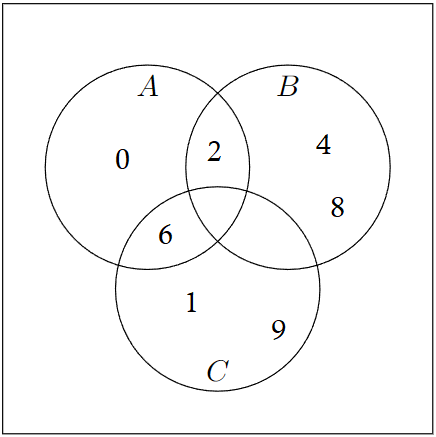
\includegraphics[height=5cm]{Venn a}
\end{figure}
    \end{center}
    
    b. $(A - B) \cap C$
    \begin{align*}
    & \noindent \text{Por definición: } A - B = A \backslash B = \forall x(x \in \{0, 6, 2\} \land x \notin \{2, 4, 8\}) = \{0, 6\} \\
    & \text{Por definición: } (A - B) \cap C = \forall x(x \in \{0, 6\} \land x \in \{1, 6, 9\}) = \{{6}\} \\
    \end{align*}

    \begin{center}
    \begin{figure}[h]
  \centering
  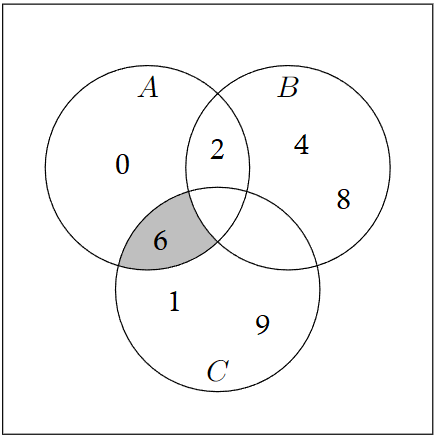
\includegraphics[height=5cm]{Venn b}
\end{figure}
    \end{center}
\newpage
    c. $(A \cup B) \cap (A \cup C)$
    \begin{align*}
    & \text{Por definición: } A \cup B = \forall x(x \in \{0, 6, 2\} \lor x \in \{2, 4, 8\}) = \{{0, 2, 4, 6, 8\}} \\
    & \text{Por definición: } A \cup C = \forall x(x \in \{0, 6, 2\} \lor x \in \{1, 6, 9\}) = \{{0, 1, 2, 6, 9\}} \\
    & \text{Por definición: } (A \cup B) \cap (A \cup C) = \forall x(x \in \{0, 2, 4, 6, 8\} \land x \in \{0, 1, 2, 6, 9\}) = \{{0, 2, 6\}} ={A} \\
    \end{align*}

    \begin{center}
    \begin{figure}[h]
  \centering
  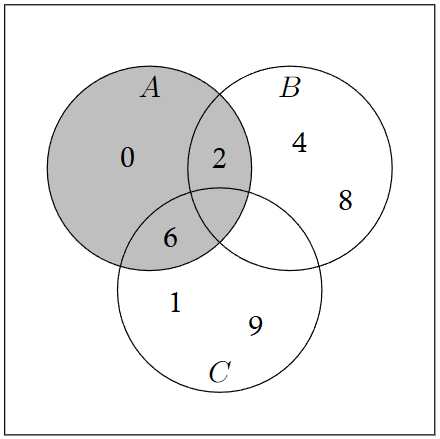
\includegraphics[height=4.55cm]{Venn c}
\end{figure}
    \end{center}
    
    d. $(A \cap B) \cup (A \cap C)$
    \begin{align*}
    & \text{Por definición: } A \cap B = \forall x(x \in \{0, 6, 2\} \land x \in \{2, 4, 8\}) = \{{2\}} \\
    & \text{Por definición: } A \cap C = \forall x(x \in \{0, 6, 2\} \land x \in \{1, 6, 9\}) = \{{6}\} \\
    & \text{Por definición: } (A \cap B) \cup (A \cap C) = \forall x(x \in \{{2\}} \lor x \in \{{6}\}) = \{{2, 6\}} \\
    \end{align*}

    \begin{center}
    \begin{figure}[h]
  \centering
  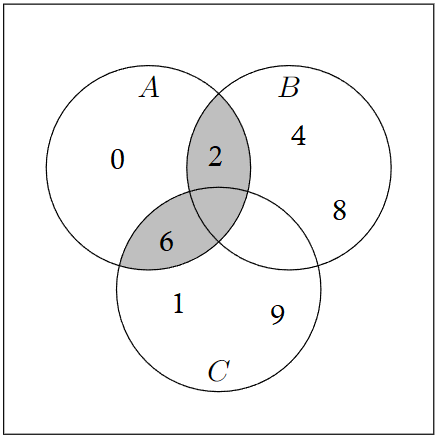
\includegraphics[height=4.55cm]{Venn d}
\end{figure}
    \end{center}

    e. $C \cap (A \cup B \cup C)$
    \begin{align*}
    & \text{Por definición: } (A \cup B \cup C) = \forall x(x \in {0, 6, 2} \lor x \in {2, 4, 8} \lor x \in {1, 6, 9}) = U \\
    & \text{Por definición: } C \cap (A \cup B \cup C) = \forall x(x \in {1, 6, 9} \land x \in U) = {1, 6, 9} \\
    \end{align*}

    \begin{center}
    \begin{figure}[h]
  \centering
  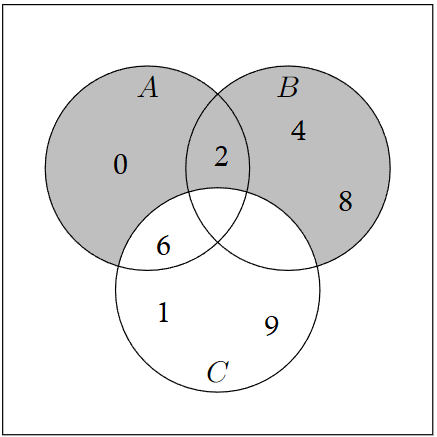
\includegraphics[height=4.55cm]{Venn e}
\end{figure}
    \end{center}

\end{enumerate}
{}
\newpage

2. Demuestra que para todo conjunto \(A\), \(B\) y \(C\):


    f. $A \cup (B \cap C)$ = $(A \cup B) \cap (A \cup C)$
Al tener una igualdad de conjuntos es necesario demostrar esto por medio de una doble contención, es decir, tomando un elemento arbitrario queremos ver que esté en el conjunto del lado izquierdo de la igualdad y al mismo tiempo dicho elemento esté en el conjunto del lado derecho. Por lo tanto.\\


\(\subseteq\)

Sea \(x \in A \cup (B \cap C)\). P.D \(x \in (A \cup B) \cap (A \cup C)\).

Por definición de unión, \(x \in A\) o \(x \in (B \cap C\)).

Por definición de intersección, \(x \in A\) o (\(x \in B\) y \(x \in C\)).

Por equivalencias lógicas, \((x \in A\) o \(x \in B)\) y \((x \in A\) o \(x \in C\)).

Por definición de intersección, \(x \in (A \cup B)\) y \(x \in (A \cup C)\).

Por definición de intersección, \(x \in (A \cup B) \cap (A \cup C)\). \\

\(\supseteq\)

Sea \(x \in (A \cup B) \cap (A \cup C)\). P.D \(x \in A \cup (B \cap C)\).

Por definición de intersección, \(x \in (A \cup B)\) y \(x \in (A \cup C)\).

Por definición de unión, \((x \in A\) o \(x \in B)\) y \((x \in A\) o \(x \in C\)).

Por equivalencias lógicas, \(x \in A\) o (\(x \in B\) y \(x \in C\)).

Por definición de intersección, \(x \in A\) o \(x \in (B \cap C)\).

Por definición de unión, \(x \in A \cup (B \cap C)\).

Hemos demostrado que \(A \cup (B \cap C) = (A \cup B) \cap (A \cup C)\).

\(\blacksquare\)\\

    g. $A \cap (B \cup C)$ = $(A \cap B) \cup (A \cap C)$\\

\(\subseteq\)

Sea \(x \in A \cap (B \cup C)\). P.D \(x \in (A \cap B) \cup (A \cap C)\).

Por definición de intersección, \(x \in A\) y \(x \in (B \cup C)\).

Por definición de unión, \(x \in A\) y (\(x \in B\) o \(x \in C\)).

Por la distribución lógica, (\(x \in A\) y \(x \in B\)) o (\(x \in A\) y \(x \in C\)).

Por definición de intersección, \(x \in (A \cap B)\) o \(x \in (A \cap C)\).

Por definición de unión, \(x \in (A \cap B) \cup (A \cap C)\). \\

\(\supseteq\)

Sea \(x \in (A \cap B) \cup (A \cap C)\). P.D \(x \in A \cap (B \cup C)\).

Por definición de unión, \(x \in (A \cap B)\) o \(x \in (A \cap C)\).

Por definición de intersección, (\(x \in A\) y \(x \in B\)) o (\(x \in A\) y \(x \in C\)).

Por la distribución lógica, \(x \in A\) y (\(x \in B\) o \(x \in C\)).

Por definición de unión, \(x \in A\) y (\(x \in B\) o \(x \in C\)).

Por definición de unión, \(x \in A\) y \(x \in (B \cup C)\).

Hemos demostrado que \(A \cap (B \cup C) = (A \cap B) \cup (A \cap C)\).

\(\blacksquare\)


\newpage
\section*{Demostraciones}

\subsection*{Definiciones}

Definición 1: \(a-b=a+(-b)\)
{}\\
Definición 2: \(\frac{a}{b}=a\frac{1}{b} = ab^{-1}\), \(b\neq 0\) \\\\

\noindent \textbf{Propiedades.} \\
3. Si \(a\) y \(b\) son números reales tales que \(a+b=0\), entonces \(b=-a\). \\
Supongamos que \(a+b=0\):
\begin{align*}
    a + b &= 0 && \text{Suposición inicial} \\
    (a + b) + (-a) &= 0 + (-a) && \text{Nociones comunes de Euclides: Suma} \\
    (b + a) + (-a) &= (-a) && \text{Axioma del elemento neutro aditivo} \\
    b + (a + (-a)) &= (-a) && \text{Axioma de la asociatividad de la adición} \\
    b + 0 &= (-a) && \text{Axioma del inverso aditivo} \\
    b &= (-a) && \text{Axioma del neutro aditivo}
\end{align*}

4. Si \(a\) es un número real cualquiera, entonces:\\
a) \quad -(-a) = a \\
Teorema doble negativo.
\begin{align*}
-(-a) &= -(-a) + 0 && \text{Nociones comunes de Euclides y axioma del neutro aditivo} \\
&= -(-a) + ((-a) + a)) && \text{Axioma del inverso aditivo} \\
&= (-(-a) + (-a)) + a && \text{Axioma de la asociatividad de la adición} \\
&= (0) + a && \text{Axioma del inverso aditivo} \\
&= a && \text{Axioma del neutro aditivo}.
\end{align*}
b) \quad (-1)a = -a \\
Teorema multiplicación negativa.
\begin{align*}
(-1)a &= (-1)a + 0 && \text{Nociones comunes de Euclides y axioma del neutro aditivo} \\
&= (-1)a + (a + (-a)) && \text{Axioma del inverso aditivo} \\
&= (-1)a + a + (-a) && \text{Axioma de la asociatividad de la adición} \\
&= (-a) + (-1)a + a && \text{Axioma de la conmutatividad de la adición} \\
&= (-a) + (-1)a + (1)a && \text{Axioma del elemento neutro en la multiplicación} \\
&= (-a) + ((-1)a + (1)a) && \text{Axioma de la asociatividad de la adición} \\
&= (-a) + ((-1)+1)(a + a) && \text{Axioma de la conmutatividad y asociatividad de la adición} \\
&= (-a) + (0)(2a) && \text{Axioma del inverso aditivo} \\
&= (-a) + 0 && \text{Existencia del cero multiplicativo} \\
&= -a && \text{Axioma del neutro aditivo}.
\end{align*}

c) \quad a(-b) = (-a)b = -ab \\
\begin{align*}
    a(-b) + ab &= a(-b) + ab && \text{Nociones comunes de Euclides} \\
    a(-b) + ab &= a((-b) + b) && \text{Axioma de la distributividad} \\
    a(-b) + ab &= a \cdot 0 && \text{Axioma del inverso aditivo} \\
    a(-b) + ab &= 0 && \text{Existencia del cero multiplicativo} \\
    (a(-b) + ab) + (-ab) &= 0 + (-ab) && \text{Axioma del inverso aditivo} \\
    a(-b) + (ab + (-ab)) &= (-ab) && \text{Axioma de la asociatividad de la adición y el neutro aditivo} \\
    a(-b) + 0 &= (-ab) && \text{Axioma del inverso aditivo} \\
    a(-b) &= (-ab) && \text{Axioma del neutro aditivo}
\end{align*}
Por otro lado.
\begin{align*}
    0 &= 0 && \text{Nociones comunes de Euclides} \\
    0 &= 0 \cdot b && \text{Existencia del cero multiplicativo} \\
    0 &= ((-a) + a)b && \text{Axioma del inverso aditivo} \\
    0 &= (-a)b + ab && \text{Axioma de la distributividad} \\
    0 + (-ab) &= ((-a)b + ab) + (-ab) && \text{Axioma del inverso aditivo} \\
    (-ab) &= (-a)b + (ab + (-ab)) && \text{Axioma de la asociatividad de la adición y el neutro aditivo} \\
    (-ab) &= (-a)b + 0 && \text{Axioma del inverso aditivo} \\
    (-ab) &= (-a)b && \text{Axioma del neutro aditivo}
\end{align*}

Por lo tanto, por transitividad, se cumple la triple igualdad: a(-b) = (-a)b = -ab\\

d) \quad (-a)(-b) = ab \\
\begin{align*}
    (-a)(-b) &= (-a)(-b) && \text{Nociones comunes de Euclides} \\
    &= (-1)(a) \cdot (-1)(b) && \text{Por teorema b} \\
    &= (-1) \cdot ((a)(-1)) \cdot (b) && \text{Axioma de la asociatividad de la multiplicación} \\
    &= (-1) \cdot ((-a)(b)) && \text{Por teorema b y asociatividad de la multiplicación} \\
    &= ((-1)(-a)) \cdot b && \text{Axioma de la asociatividad de la multiplicación} \\
    &= - (-a) \cdot b && \text{Teorema multiplicación negativa (teorema b)} \\
    &= a \cdot b && \text{Teorema doble negativo (teorema a)}
\end{align*}


e) \quad \((ab)^{-1} = a^{-1}b^{-1}, \quad a\neq 0, b\neq 0 \) \\
Teorema. Distributividad de potencias.\\
\begin{align*}
    1 &= 1 && \text{Nociones comunes de Euclides} \\
    a(a^{-1}) &= 1 && \text{Axioma del inverso multiplicativo} \\
    1 \cdot (a(a^{-1})) &= 1 && \text{Axioma del neutro multiplicativo} \\
    (b(b^{-1})) \cdot (a(a^{-1})) &= 1 && \text{Axioma del inverso multiplicativo} \\
    (b(b^{-1})) \cdot ((a^{-1})a) &= 1 && \text{Axioma de la conmutatividad de la multiplicación} \\
    b \cdot ((b^{-1})(a^{-1})) \cdot a &= 1 && \text{Axioma de la asociatividad de la multiplicación} \\
    ((b^{-1})(a^{-1})) \cdot (ab) &= 1 && \text{Axioma de la conmutatividad de la multiplicación} \\
    (((b^{-1})(a^{-1})) \cdot (ab)) \cdot ((ab)^{-1}) &= (ab)^{-1} && \text{Axioma del inverso multiplicativo y el neutro multiplicativo} \\
    ((b^{-1})(a^{-1})) \cdot (ab \cdot (ab)^{-1})) &= (ab)^{-1} && \text{Axioma de la asociatividad de la multiplicación} \\
    ((b^{-1})(a^{-1})) \cdot (1)&= (ab)^{-1} && \text{Axioma del inverso multiplicativo} \\
    ((b^{-1})(a^{-1})) &= (ab)^{-1} && \text{Axioma del neutro multiplicativo} \\
    (a^{-1})(b^{-1}) &= (ab)^{-1} && \text{Axioma de la conmutatividad de la multiplicación}
\end{align*}

f) \quad \( \frac{a}{b} \cdot \frac{c}{d} = \frac{ac}{bd}, \quad b\neq 0, d\neq 0 \) \\
\begin{align*}
    \frac{a}{b} \cdot \frac{c}{d} &= (ab^{-1})(cd^{-1}) && \text{Por definición axiomática esta igualdad se cumple} \\
    &= (b^{-1}a)(cd^{-1}) && \text{Axioma de la conmutatividad de la multiplicación} \\
    &= (ac)(b^{-1}d^{-1}) && \text{Axioma de la asociatividad y conmutatividad de la multiplicación} \\
    &= (ac)(bd)^{-1} && \text{Distributividad de potencias (teorema e)} \\
    &= \frac{ac}{bd} && \text{Por definición de inverso multiplicativo} \\
\end{align*}

\newpage
g) \quad \( \frac{a}{c} + \frac{b}{c} = \frac{a+b}{c}, \quad c\neq 0 \) \\
\begin{align*}
    \frac{a}{c} + \frac{b}{c} &= ac^{-1} + bc^{-1} && \text{Por definición axiomática esta igualdad se cumple} \\
    &= c^{-1}(a+b) && \text{Axioma de la distributividad} \\
    &= (a+b)c^{-1} && \text{Axioma de la conmutatividad de la multiplicación} \\
    &= \frac{a+b}{c} && \text{Por definición de inverso multiplicativo} \\
\end{align*}

h) \quad \( \frac{a}{b} + \frac{c}{d} = \frac{ad+bc}{bd}, \quad b\neq 0, d\neq \) \\
\begin{align*}
    \frac{a}{b} + \frac{c}{d} &= ab^{-1} + cd^{-1} && \text{Por definición axiomática esta igualdad se cumple} \\
    &= (ab^{-1})(1) + (cd^{-1})(1) && \text{Axioma del neutro multiplicativo} \\
    &= (ab^{-1})(d \cdot d^{-1}) + (cd^{-1})(b \cdot b^{-1}) && \text{Axioma de inverso multiplicativo} \\
    &= (ad)(b^{-1} \cdot d^{-1}) + (cb)(b^{-1} \cdot d^{-1}) && \text{Axioma de la asociatividad de la multiplicación} \\
    &= (ad)(bd)^{-1} + (cb)(bd)^{-1} && \text{Distributividad de potencias (teorema e)} \\
    &= (ad + cb)(bd)^{-1} && \text{Axioma de la distributividad} \\
    &= \frac{(ad) + (cb)}{bd} && \text{Por definición de inverso multiplicativo} \\
\end{align*}


{}
5. Si \(a\) es un número real tal que \(a>0\), entonces \(1/a > 0\). \\
\begin{proof}\text{Sea \(a\) un número real distinto del cero, supungamos que entonces es mayor que cero}
\begin{align*}
    1 &> 0 && \text{Nociones comunes de Euclides} \\
    a \cdot a^{-1} &> 0 && \text{Definición de inverso multiplicativo} \\
\end{align*}

Para que un producto sea mayor que 0, ambos factores deben ser mayores a 0 o ambos deben ser menores a 0:

\[ a \cdot a^{-1} > 0 \iff (a > 0 \land a^{-1} > 0) \lor (a < 0 \land a^{-1} < 0) \]
Sin embargo, la hipótesis nos indica que \(a\) es mayor a 0, por lo tanto, se descarta el segundo caso.
\[ a \cdot a^{-1} > 0 \iff (a > 0 \land a^{-1} > 0) \]
Por esta condición, tenemos también que \(a > 0\) por lo tanto podemos multiplicar a ambos lados de la desigualdad por el inverso multiplicativo de este número real \(a\), pues \(a\) es estrictamente mayor que 0 y para que exista un inverso multiplicativo el número real debe ser distinto del cero:
\[ a^{-1}(a \cdot a^{-1}) > 0(a^{-1})  \]

Asociamos los términos de la siguiente manera y recordemos que 0 multiplicado por cualquier número es 0:

\[ (a^{-1}a) \cdot a^{-1} > 0(a^{-1})  \]
\[ (1) \cdot a^{-1} > 0  \]

\[ \therefore a^{-1} > 0 \]
\end{proof}

6. Si \(a\) es un número real tal que \(a<0\), entonces \(1/a < 0\). \\
\begin{proof}\text{Sea \(a\) un número real distinto del cero, supungamos que entonces es menor que cero}

\begin{center}

\begin{align*}
-1 &< 0 && \text{Nociones comunes de Euclides} \\ 
(-1) \cdot 1 &< 0 && \text{Neutro multiplicativo} \\
(-1)(a \cdot a^{-1}) &< 0 && \text{Inversos multiplicativos} \\
(-1)(a^{-1} \cdot a) &< 0 && \text{Conmutatividad multiplicativa} \\
((-1)(a^{-1})) \cdot a &< 0 && \text{Asociatividad multiplicativa} \\
-(a^{-1}) \cdot a &< 0 && \text{Por teorema ya demostrado $(-1)a=-a$}
\end{align*}
\end{center}

Para que un producto sea menor a 0, un factor debe ser mayor a 0 y el otro factor debe ser menor a 0, por lo que existen dos casos.

\[ -(a^{-1}) \cdot a < 0 \iff (a > 0 \land -(a^{-1}) < 0) \lor (a < 0 \land -(a^{-1}) > 0) \]

Sin embargo, la hipótesis nos indica que \(a\) es menor a 0, por lo tanto, se descarta el primer caso.

\[ -(a^{-1}) \cdot a < 0 \iff (a < 0 \land -(a^{-1}) > 0) \]

Por lo que:
\begin{center}
\begin{align*}
-(a^{-1}) &> 0 && \text{Condición necesaria} \\ 
-(a^{-1})+(a^{-1}) &> 0+(a^{-1}) && \text{Sumamos a ambos lados de la desigualdad \((a^{-1})\)} \\
0 &> (a^{-1}) && \text{Por inversos aditivos y el neutro aditivo} \\
\end{align*}
\end{center}
\[ \therefore a^{-1} < 0 \]
\end{proof}

\subsection*{Orden y desigualdades}

Definición: \(b<a\) si y solo si \(a-b\) es positivo. En particular, \(a-0=a\) es positivo si y solo si \(0<a\).\\\\
{}
  7. Sean \(a\), \(b\), y \(c\) números reales. Si \(a>b\) y \(c<0\), entonces \(ac<bc\).\\
  \begin{proof} $ac<bc$.\\
  Como \(c<0 \Rightarrow 0-c>0\)
\begin{align*}
a &> b && \text{Hipótesis} \\
(-c)a &> b(-c) && \text{Multiplicamos por } (-c) \text{ en ambos lados, por axioma de multiplicatividad la desigualdad se mantiene} \\
-ac &> -bc && \text{Por conmutatividad y teorema ya demostrado:} -a(b) = -(ab) \\
-ac+bc &> -bc+bc && \text{Sumamos a ambos lados el término } (bc) \\
bc-ac &> 0 && \text{Conmutativdad e inversos aditivos} \\
ac &< bc && \text{Aplicamos la definición} \\
\end{align*}
\end{proof}
  
  8. Si \(ab>0\), si y solo si \(a>0\) y \(b>0\), o \(a<0\) y \(b<0\).\\
\begin{align*}
\text{$\Rightarrow$}\\
&\quad \text{Supongámos que sean } a \text{ y } b \in \mathbb{R} \text{ tal que } ab > 0 \\
&\quad \text{Queremos demostrar que } (a > 0 \land b > 0) \lor (a < 0 \land b < 0) \\
&\quad \text{Dado que } ab > 0 \Rightarrow ab \neq 0, \text{ por lo tanto, } a \neq 0 \land b \neq 0 \\
&\quad \text{Como } a \neq 0 \Rightarrow a > 0 \lor a < 0 \\
&\quad \text{Como } b \neq 0 \Rightarrow b > 0 \lor b < 0 \\
&\quad \text{Entonces, como cada variable puede tener 2 valores, obtenemos 4 casos.} \\
&\quad \text{1ª Caso } a > 0 \land b > 0 \\
&\quad \quad a > 0 \\
&\quad \quad ab > 0 \quad \text{(Multiplicamos ambos lados por \(b\) y por axioma la desigualdad se mantiene)} \\
&\quad \quad ab > 0 \\
&\quad \text{2ª Caso } a > 0 \land b < 0 \\
&\quad \quad \text{Como } b < 0 \Rightarrow 0 - b > 0 \\
&\quad \quad a > 0 \\
&\quad \quad a(-b) > 0(-b) \quad \text{(por axioma de multiplicatividad la desigualdad se mantiene)} \\
&\quad \quad -ab > 0 \\
&\quad \quad ab < 0 \quad \text{(contradicción: por lo que la hipótesis del 2ª caso es falsa)} \\
&\quad \text{3ª Caso } a < 0 \land b > 0 \\
&\quad \quad \text{Como } a < 0 \Rightarrow 0 - a > 0 \\
&\quad \quad b > 0 \\
&\quad \quad b(-a) > 0(-a) \quad \text{(por axioma de multiplicatividad la desigualdad se mantiene)} \\
&\quad \quad -ab > 0 \\
&\quad \quad ab < 0 \quad \text{(contradicción: por lo que la hipótesis del 3ª caso es falsa)} \\
&\quad \text{4ª Caso } a < 0 \land b < 0 \\
&\quad \quad \text{Como } a < 0 \Rightarrow 0 - a > 0 \\
&\quad \quad \text{Como } b < 0 \Rightarrow 0 - b > 0 \\
&\quad \quad -a > 0 \\
&\quad \quad (-a)(-b) > 0(-b) \quad \text{(por axioma de multiplicatividad la desigualdad se mantiene)} \\
&\quad \quad ab > 0 \\
&\quad \text{Por lo tanto, } ab > 0 \text{ se cumple solo en los casos 1 y 4.} \\
&\quad \text{Entonces, } ab > 0 \Rightarrow (a > 0 \land b > 0) \lor (a < 0 \land b < 0) \\
\\
\text{$\Leftarrow$}\\
&\quad \text{Supongámos que sean } a \text{ y } b \in \mathbb{R} \text{ tal que } a > 0 \land b > 0 \\
&\quad \text{Queremos demostrar que } ab > 0 \\
&\quad a > 0 \\
&\quad ab > 0 \quad \text{(por axioma de multiplicatividad la desigualdad se mantiene)} \\
&\quad ab > 0 \\
\\
&\quad \text{Supongámos que sean } a \text{ y } b \in \mathbb{R} \text{ tal que } a < 0 \land b < 0 \\
&\quad \text{Queremos demostrar que } ab > 0 \\
&\quad \text{Como } a < 0 \Rightarrow 0 - a > 0 \\
&\quad \text{Como } b < 0 \Rightarrow 0 - b > 0 \\
&\quad -a > 0 \\
&\quad (-a)(-b) > 0(-b) \quad \text{(por axioma de multiplicatividad la desigualdad se mantiene)} \\
&\quad ab > 0 \\
\\
&\quad \text{Por lo tanto, } (a > 0 \land b > 0) \lor (a < 0 \land b < 0) \Rightarrow ab > 0 \\
\\
&\quad \text{Como se cumple la doble implicación, se cumple el sí y solo sí:} \\
&\quad ab > 0 \iff (a > 0 \land b > 0) \lor (a < 0 \land b < 0)
\end{align*}

  \newpage
  9. Si \(ab<0\), si y solo si \(a<0\) y \(b>0\), o bien \(a>0\) y \(b<0\).\\

Como se trata de un sí y sólo si, se debe cumplir la doble implicación, por lo que haremos una idea y un regreso.

\text{$\Rightarrow$}\\
Supóngase que $a$ y $b \in \mathbb{R}$, $ab < 0$. Se quiere demostrar que $(a < 0 \land b > 0) \lor (a > 0 \land b < 0)$.

Como $ab < 0 \implies ab \neq 0$, por lo tanto, $a \neq 0 \land b \neq 0$.

Como $a \neq 0 \implies a > 0 \lor a < 0$.

Como $b \neq 0 \implies b > 0 \lor b < 0$.

Hipótesis por tricotomía. Además, para que un producto sea distinto de 0, ningún factor debe ser 0.
Como cada variable puede tener dos valores, obtenemos cuatro casos.

\begin{align*}
&\quad \text{1ª Caso } a > 0 \land b > 0 \\
&\quad \quad a > 0 \\
&\quad \quad ab > 0 \quad \text{(Multiplicamos ambos lados por \(b\) y por axioma la desigualdad se mantiene)} \\
&\quad \quad ab > 0 \quad \text{(contradicción: por lo que la hipótesis del 1ª caso es falsa)}\\
&\quad \text{2ª Caso } a > 0 \land b < 0 \\
&\quad \quad \text{Como } b < 0 \Rightarrow 0 - b > 0 \\
&\quad \quad a > 0 \\
&\quad \quad a(-b) > 0(-b) \quad \text{(por axioma de multiplicatividad la desigualdad se mantiene)} \\
&\quad \quad -ab > 0 \\
&\quad \quad ab < 0 \\
&\quad \text{3ª Caso } a < 0 \land b > 0 \\
&\quad \quad \text{Como } a < 0 \Rightarrow 0 - a > 0 \\
&\quad \quad b > 0 \\
&\quad \quad b(-a) > 0(-a) \quad \text{(por axioma de multiplicatividad la desigualdad se mantiene)} \\
&\quad \quad -ab > 0 \\
&\quad \quad ab < 0 \\
&\quad \text{4ª Caso } a < 0 \land b < 0 \\
&\quad \quad \text{Como } a < 0 \Rightarrow 0 - a > 0 \\
&\quad \quad \text{Como } b < 0 \Rightarrow 0 - b > 0 \\
&\quad \quad -a > 0 \\
&\quad \quad (-a)(-b) > 0(-b) \quad \text{(por axioma de multiplicatividad la desigualdad se mantiene)} \\
&\quad \quad ab > 0 \quad \text{(contradicción: por lo que la hipótesis del 4ª caso es falsa)} \\
&\quad \text{Por lo tanto, } ab < 0 \text{ se cumple solo en los casos 2 y 3.} \\
&\quad \text{Entonces, } ab < 0 \Rightarrow (a < 0 \land b > 0) \lor (a>0 \land b<0) \\
\\
\text{$\Leftarrow$}\\
&\quad \text{Supongámos que sean } a \text{ y } b \in \mathbb{R} \text{ tal que } a < 0 \land b > 0 \\
&\quad \text{Queremos demostrar que } ab < 0 \\
&\quad a < 0 \\
&\quad ab < 0 \quad \text{(por axioma de multiplicatividad la desigualdad se mantiene)} \\
&\quad ab < 0 \\
\\
&\quad \text{Supongámos que sean } a \text{ y } b \in \mathbb{R} \text{ tal que } a > 0 \land b < 0 \\
&\quad \text{Queremos demostrar que } ab < 0 \\
&\quad b < 0 \\
&\quad ab < 0a \quad \text{(por axioma de multiplicatividad la desigualdad se mantiene)} \\
&\quad ab < 0 \\
&\quad \text{Por lo tanto, } (a < 0 \land b > 0) \lor (a > 0 \land b < 0) \Rightarrow ab < 0 \\
\\
&\quad \text{Como se cumple la doble implicación, se cumple el sí y solo sí:} \\
&\quad ab < 0 \iff (a > 0 \land b < 0) \lor (a > 0 \land b < 0)
\end{align*}


  \newpage
  10. Si \(0<a<b\), entonces \(a<\sqrt{ab}<\frac{a+b}{2}<b\).
\begin{proof}
\(0<a<b \Rightarrow a < \sqrt{ab} < \frac{a+b}{2} < b\)\\

\textit{Demostraremos que \(\frac{a+b}{2}\) está entre a y b}\\
\[a<b\]
\begin{alignat*}{2}
a + a &< a + b \quad && \quad a + b < b + b \\
2a &< a + b \quad &&  \quad a + b < 2b \\
\frac{2a}{2} &< \frac{a + b}{2} \quad && \quad \frac{a + b}{2} < \frac{2b}{2} \\
a &< \frac{a + b}{2} \quad && \quad \frac{a + b}{2} < b \\
\end{alignat*}
\[a <  \frac{a + b}{2} < b\]
    
\textit{Ahora demostraremos que \(a<\sqrt{ab}<b\) por Reducción al Absurdo}\\
Consideramos las siguientes propiedades: \(0<a<b \wedge 0<ab\)
supongamos, por el contrario, que \[a>\sqrt{ab}>b\]
\begin{alignat*}{2}
a > \sqrt{ab} \quad && \quad \sqrt{ab} > b \\
a^2 > \sqrt{ab}^2 \quad && \quad \sqrt{ab}^2 > b^2 \\
a^2 > |ab| \quad && \quad |ab| > b^2 \\
a^2 > ab \quad && \quad ab > b^2 \\
\frac{a^2}{a} > \frac{ab}{a} \quad && \quad \frac{ab}{b} > \frac{b^2}{b} \\
a > b \circledast \quad && \quad a > b \circledast
\end{alignat*}
\textit{Hemos llegado a algo falso al suponer lo contrario} \\
\( \therefore a<\sqrt{ab}<b\) \\

\textit{Ahora demostraremos que \(\sqrt{ab}<\frac{a+b}{2}\)} \\
\begin{align*}
a &< b \\
\sqrt{a} &< \sqrt{b} \\
0 &< \sqrt{b} - \sqrt{a} \\
0^2 &< (\sqrt{b} - \sqrt{a})^2 \\
0 &< b - 2\sqrt{a}\sqrt{b} + a \\
2\sqrt{a}\sqrt{b} &< a + b \\
\frac{2\sqrt{ab}}{2} &< \frac{a + b}{2} \\
\sqrt{ab} &< \frac{a + b}{2} \\
\end{align*}

\textit{Finalmente vemos las desigualdades que tenemos y por transitividad}
\[a <  \frac{a + b}{2} < b\]
\[a < \sqrt{ab} < b\]
\[\sqrt{ab} < \frac{a + b}{2} \]
\[ \therefore a<\sqrt{ab}<\frac{a+b}{2}<b\]

\end{proof}

\section*{Desigualdades}

\subsection*{11. Obtén el conjunto solución de:}

\begin{enumerate}
  \item \(4x-5<7x-4\)
  \begin{align*}
  4x - 5 + 5 - 7x & < 7x - 4 + 5 - 7x && \text{Sumar } 5 \text{ a ambos lados y restar } 7x \text{ a ambos lados} \\
   -3x & < 1 && \text{Simplificar} \\
   (-1)(-3x) & > 1(-1) && \text{Multiplicar por } (-1) \text{ en ambos lados} \\
   3x & > -1 && \text{Simplificar} \\
   \frac{3x}{3} & > -\frac{1}{3} && \text{Dividir por } 3 \text{ en ambos lados} \\
   x & > -\frac{1}{3} && \text{Simplificar} \\
   \end{align*}
   Por lo tanto, la solución es \(x \in \left(-\frac{1}{3}, +\infty\right)\).\\

   
  \item \(x<\frac{5x-2}{2}<7-x\)
  
Estos casos son llamados como dobles desigualdades porque, claramente por trsnsitivdad, queremos que se cumplan dos casos:
\begin{align*}
   x & < \frac{5x - 2}{2} && \text{Primera desigualdad} \\
   \frac{5x - 2}{2} & < 7 - x && \text{Segunda desigualdad} \\
   \end{align*}
   
   Entonces como ambos casos queremos que se cumplan, podemos ocupar el conectivo lógico “y", llamado conjunción, lo cual nos indicara después, que el conjunto solución de esta doble desigualdad será la intersección de los conjuntos obtenidos en cada desigualdad por separado, pues ambos se deben cumplir. En la primera inecuación tenemos que:
   \begin{align*}
   x - x & < \frac{5x - 2}{2} - x && \text{Restar } x \text{ a ambos lados} \\
   0 & < \frac{5x - 2 - 2x}{2} && \text{Simplificar} \\
   0 & < \frac{3x - 2}{2} && \text{Simplificar} \\
   \frac{2(3x - 2)}{2} & > {0}(2) && \text{Multiplicar por } 2 \text{ en ambos lados} \\
   3x - 2 & > 0 && \text{Simplificar} \\
   3x - 2 + 2 & > 0 + 2 && \text{Sumar } 2 \text{ a ambos lados} \\
   3x & > 2 && \text{Simplificar} \\
   \frac{3x}{3} & > \frac{2}{3} && \text{Dividir por } 3 \text{ en ambos lados} \\
   x & > \frac{2}{3} && \text{Simplificar} \\
   \end{align*}
   La solución para la primera desigualdad es \(x \in \left(\frac{2}{3}, +\infty\right)\).
   
   Para la segunda inecuación:
   \begin{align*}
   \frac{5x - 2}{2} - 7 + x & < 0 && \text{Restar } 7 \text{ y sumar } x \text{ a ambos lados} \\
   \frac{5x - 2 - 14 + 2x}{2} & < 0 && \text{Simplificar} \\
   \frac{7x - 16}{2} & < 0 && \text{Simplificar} \\
   2\left(\frac{7x - 16}{2}\right) & > 2(0) && \text{Multiplicar por } 2 \text{ en ambos lados} \\
   7x - 16 & < 0 && \text{Simplificar} \\
   7x - 16 + 16 & < 0 + 16 && \text{Sumar } 16 \text{ a ambos lados} \\
   7x & < 16 && \text{Simplificar} \\
   \frac{7x}{7} & < \frac{16}{7} && \text{Dividir por } 7 \text{ en ambos lados} \\
   x & < \frac{16}{7} && \text{Simplificar} \\
   \end{align*}
   La solución para la segunda desigualdad es \(x \in \left(-\infty, \frac{16}{7}\right)\).
   
   Para encontrar la intersección de ambos conjuntos de soluciones, tomamos la intersección de los intervalos:
   \[x \in \left(\frac{2}{3}, +\infty\right) \cap \left(-\infty, \frac{16}{7}\right) = \left(\frac{2}{3}, \frac{16}{7}\right)\]
   Por lo tanto, la solución es \(x \in \left(\frac{2}{3}, \frac{16}{7}\right)\)

  
  \item \(\frac{3}{x+5}<x\) \\

Dado que $x$ se encuentra en una división, es necesario restringir en qué valores no está definida:

\[
\begin{aligned}
    x + 5 &= 0 \\
    x + 5 - 5 &= -5 \\
    x &= -5
\end{aligned}
\]

Por lo tanto, $x \neq -5$. Con esto en consideración, podemos realizar lo siguiente:

\[
\begin{aligned}
    \frac{3}{x + 5} - x &< x - x \\
    \frac{3}{x + 5} - x &< 0 \\
    \frac{3 - x^2 - 5x}{x + 5} &< 0
\end{aligned}
\]

Dado que tenemos una división entre dos números que debe ser menor que 0, según lo que hemos visto, esto ocurre si se cumplen alguno de los siguientes casos:

\begin{align*}
\textit{Condición 1} = 
\left\{
\begin{array}{rcl}
{3-x^2-5x<0}\\
x+5>0
\end{array}\right.
\end{align*}

\begin{align*}
\textit{Condición 2} =
\left\{
\begin{array}{rcl}
{3-x^2-5x>0}\\
x+5<0
\end{array}\right.
\end{align*}

Empecemos con la condición 1:

\begin{align*}
    3 - x^2 - 5x &< 0 \\
    -x^2 - 5x + 3 &< 0
\end{align*}

Como la ecuación cuadrática es menor que cero, busquemos donde da como resultado 0:

\begin{align*}
    -x^2 - 5x + 3 &= 0 \\
    \text{Resolvamos por completar el cuadrado perfecto:} \\
    -x^2 - 5x + 3 - 3 &= 0 - 3 \\
    -x^2 - 5x &= -3 \\
    -(-x^2 - 5x) &= -(-3) \\
    x^2 + 5x &= 3 \\
    (x)^2 + 2(x)\left(\frac{5}{2}\right) + \left(\frac{5}{2}\right)^2 &= 3 + \left(\frac{5}{2}\right)^2 \\
    (x + \frac{5}{2})^2 &= \frac{12}{4} + \frac{25}{4} \\
    (x + \frac{5}{2})^2 &= \frac{37}{4} \\
    \sqrt{(x + \frac{5}{2})^2} &= \pm \sqrt{\frac{37}{4}} \\
    x + \frac{5}{2} - \frac{5}{2} &= \pm \frac{\sqrt{37}}{\sqrt{4}} - \frac{5}{2} \\
    x &= -\frac{5}{2} \pm \frac{\sqrt{37}}{2}
\end{align*}

Por lo tanto, $x_1 = \frac{-5 + \sqrt{37}}{2} \approx 0.54138$ y $x_2 = \frac{-5 - \sqrt{37}}{2} \approx -5.54138$.

Ahora bien, se obtuvieron las dos soluciones de la ecuación cuadrática para poder encontrar el conjunto solución de la expresión $3 - x^2 - 5x$ cuando esta es menor que 0. Recordemos que esta expresión se puede escribir como la ecuación $-x^2 - 5x + 3 = 0$, donde gráficamente representa una parábola. Para determinar en qué intervalos sus imágenes son menores que cero, basta con saber cuál es su concavidad.

Para determinar la concavidad, solo tenemos que fijarnos en el signo del coeficiente líder o término cuadrático; en este caso, es \(-1\), por lo que la concavidad de esta parábola es hacia abajo. Además, los puntos de intersección con el eje \(x\) (los ceros o soluciones de la ecuación) nos determinan los cambios de concavidad. Esto quiere decir que en los intervalos de:

\[
\begin{aligned}
    (-\infty, \frac{-5 - \sqrt{37}}{2}) \\
\text{Y de} \\
    (\frac{-5 + \sqrt{37}}{2}, +\infty)
\end{aligned}
\]

La parábola es cuando es menor a 0, y por lo tanto de $\left(\frac{-5-\sqrt{37}}{2},\frac{-5+\sqrt{37}}{2}\right)$ es cuando ésta adquiere valores mayores a 0.

\[ x \in (-\infty, \frac{-5-\sqrt{37}}{2}) \cup (\frac{-5+\sqrt{37}}{2}, +\infty) \]

En la segunda inecuación tenemos lo siguiente:

\[ x + 5 > 0 \Rightarrow x + 5 - 5 > 0 - 5 \Rightarrow x > -5 \Rightarrow x \in (-5, +\infty) \]

Como estas fueron las condiciones del primer caso, hay que calcular la intersección entre estos conjuntos, ya que ambas condiciones se deben cumplir simultáneamente.

\[ \left( (-\infty, \frac{-5-\sqrt{37}}{2}) \cup (\frac{-5+\sqrt{37}}{2}, +\infty) \right) \cap (-5, +\infty) = \left( \frac{-5+\sqrt{37}}{2}, +\infty \right) \]

Por lo tanto, \( x \in \left( \frac{-5+\sqrt{37}}{2}, +\infty \right) \).

Pasemos con la condición 2:

\[ 3 - x^2 - 5x > 0 \]

\[ -x^2 - 5x + 3 > 0 \]

En la primera inecuación, como vimos en el análisis anterior, la expresamos como una ecuación cuadrática para que, a partir de los ceros-soluciones de la parábola que ésta representa gráficamente, pudiéramos encontrar más rápidamente el conjunto solución. En este caso, queremos que sea mayor que 0, como fue determinado. Esto pasará cuando:

\[ x \in \left( \frac{-5-\sqrt{37}}{2}, \frac{-5+\sqrt{37}}{2} \right) \]

Por su parte, en la segunda inecuación tenemos que:

\[ x + 5 - 5 < 0 - 5 \Rightarrow x < -5 \Rightarrow x \in (-\infty, -5) \]

Y como estas condiciones son del segundo caso, hay que calcular la intersección entre estos conjuntos, pues ambas condiciones se deben cumplir simultáneamente:

\[ \left( \frac{-5-\sqrt{37}}{2}, \frac{-5+\sqrt{37}}{2} \right) \cap (-\infty, -5) = \left( \frac{-5-\sqrt{37}}{2}, -5 \right) \]

Por lo tanto, \( x \in \left( \frac{-5-\sqrt{37}}{2}, -5 \right) \)

Sin embargo, recordemos que, en un inicio, teníamos la expresión \( \frac{3 - x^2 - 5x}{x + 5} < 0 \). Por lo tanto, pasa un caso o pasa el otro. Así que, habrá que calcular la unión entre los últimos conjuntos de soluciones obtenidos para saber el conjunto solución de la inecuación en total:

\[ x \in \left( \frac{-5-\sqrt{37}}{2}, -5 \right) \cup \left( \frac{-5+\sqrt{37}}{2}, +\infty \right), \quad x = -5 \]

Por lo tanto, la solución es \( x \in \left( \frac{-5-\sqrt{37}}{2}, -5 \right) \cup \left( \frac{-5+\sqrt{37}}{2}, +\infty \right) \).\\
  
  \item \(x^2<4x\)

Se restará por ambos lados de la desigualdad \(4x\) para luego factorizar la expresión del lado izquierdo.

\[ x^2 - 4x < 4x - 4x \Rightarrow x^2 - 4x < 0 \Rightarrow x(x-4) < 0 \]

A continuación, se dividirá por casos, pues el producto entre dos números es menor que 0 cuando el primer factor es negativo y el segundo es positivo, o cuando el primer factor es mayor que cero y el segundo es menor que cero. Al final, se unirán los conjuntos de solución obtenidos, pues pasa un caso o pasa el otro, y así hallar el conjunto solución de la inecuación en general.

Caso 1: \(x < 0\) y \(x-4 > 0\)

\[ x < 0 \quad \text{y} \quad x > 4 \]

\[\therefore x \in (-\infty, 0) \cap (4, +\infty) = \emptyset \]

\[\therefore \text{El primer caso se descarta, pues no tiene ninguna solución}\]

Caso 2: \(x > 0\) y \(x-4 < 0\)

\[ x > 0 \quad \text{y} \quad x < 4 \]

\[\therefore x \in (0, +\infty) \cap (-\infty, 4)\]

\[\therefore \text{La solución es } x \in (0,4)\]

Pues el vacío unión con cualquier conjunto, \(\emptyset \cup (0,4)\), siempre da el mismo conjunto. En una unión queremos saber qué elementos pertenecen al primer conjunto Ó al segundo (sin importar que estos compartan o no alguno en común), y como ya se cumple una de las condiciones, en este caso que \(x \in (0,4)\), entonces el otro disyunto se cumple, pues para que una disyunción (como lo es la unión entre conjuntos) sea verdadera, al menos uno de los dos es verdadero.

Como el primero es el vacío y el vacío no tiene elementos, entonces automáticamente la unión del vacío con cualquier otro conjunto es el mismo conjunto, pues hay que demostrar que al menos hay un elemento que pertenece al vacío o que éste pertenezca al segundo conjunto. PERO EL VACÍO NO TIENE ELEMENTOS. Es por esta razón que la unión resulta ser el intervalo \((0,4)\), y este es el conjunto solución de la desigualdad.


  \item \(x^2\leq x+2\)
  
Restamos por ambos lados de la desigualdad el término \((x+2)\) y hacemos los cálculos correspondientes:

\[ x^2 - x - 2 \leq 0 \quad (\text{Ahora, expresamos al término } (-x) \text{ como una diferencia para después poder factorizar}) \]

\[ x^2 + x - 2x - 2 \leq 0 \quad (\text{Factorizamos}) \]

\[ x(x+1) - 2(x+1) \leq 0 \quad (\text{Sacamos el factor común de ambas expresiones } (x+1)) \]

\[ (x+1)(x-2) \leq 0 \quad (\text{Dividimos por dos posibles casos para hallar el conjunto solución}) \]

Caso 1:
\[ x+1 \leq 0 \quad \text{y} \quad x-2 \geq 0 \]
\[ x \leq -1 \quad \text{y} \quad x \geq 2 \]
\[ x \in (-\infty, -1] \quad \text{y} \quad x \in [2, +\infty) \]
\[\therefore x \in (-\infty, -1] \cap [2, +\infty)\]

\[(-\infty, -1] \cap [2, +\infty) = \emptyset \quad (\text{La intersección de ambos es el vacío } \emptyset )\]

Caso 2:
\[ x+1 \geq 0 \quad \text{y} \quad x-2 \leq 0 \]
\[ x \geq -1 \quad \text{y} \quad x \leq 2 \]
\[ x \in [-1, +\infty) \quad \text{y} \quad x \in (-\infty, 2] \]
\[\therefore x \in [-1, +\infty) \cap (-\infty, 2]\]

\[\therefore \text{La intersección de ambos es el intervalo } x \in [-1, 2]\]

Entonces, para hallar el conjunto solución, hacemos la unión entre ambos casos, por lo que la solución es:

\[ x \in [-1,2] \cup \emptyset \quad \therefore x \in [-1,2] \]\\


  \item \(\frac{x}{1-x}\geq\frac{2+x}{x}\)

Restamos por ambos lados el término $\frac{2+x}{x}$ y hacemos los cálculos correspondientes:
\[
\frac{x}{1-x} - \frac{2+x}{x} \geq 0 \quad \text{(Resta de quebrados)}
\]
\[
\frac{x(x) - (1-x)(2+x)}{x(1-x)} \geq 0 \quad \text{(Simplificamos la expresión)}
\]
\[
\frac{x^2 - (2-x-x^2)}{x(1-x)} \geq 0 \quad \text{(Multiplicamos por el signo)}
\]
\[
\frac{x^2 - 2 + x + x^2}{x(1-x)} \geq 0 \quad \text{(Agrupamos términos semejantes y aplicamos el axioma de conmutatividad)}
\]
\[
\frac{2x^2 + x - 2}{x(1-x)} \geq 0
\]

Como tenemos una división, \(x\) deberá restringirse en los valores que hagan que el denominador sea 0:
\[
x(1-x) = 0 \quad \therefore x = 0 \text{ o } 1-x = 0, \text{ es decir: } x \neq 1 \text{ y } x \neq 0
\]

Teniendo entonces dos posibles casos en general:

\textbf{Caso 1:}
\[
2x^2 + x - 2 \geq 0 \quad \text{(Para el numerador de la desigualdad)}
\]
\[
2x^2 + x - 2 = 0 \quad \text{(Escribimos en términos de la fórmula cuadrática,)}
\]
\[
x = \frac{-1 \pm \sqrt{1^2 - 4(2)(-2)}}{2(2)} \quad \text{(Calculamos)}
\]
\[
x_1 = \frac{-1 + \sqrt{17}}{4} \approx 0.7807 \quad \text{o} \quad x_2 = \frac{-1 - \sqrt{17}}{4} \approx -1.2807
\]
Por lo que, en donde la expresión \(2x^2 + x - 2 = 0\) (que gráficamente representa una parábola) será mayor o igual que 0 (esta era la condición original) cuando:
\[
x \in \left[ \frac{-1 + \sqrt{17}}{4}, +\infty \right) \quad \text{o} \quad x \in \left(-\infty, \frac{-1 - \sqrt{17}}{4}\right]
\]

Entonces, como \(x\) pertenece a un intervalo o al otro, calculamos su unión:
\[
x \in \left(-\infty, \frac{-1 - \sqrt{17}}{4}\right] \cup \left[\frac{-1 + \sqrt{17}}{4}, +\infty\right)
\]

Pasemos ahora con los casos del denominador de la desigualdad, para el \textbf{Caso 1}:
\[
x(1-x) > 0
\]

Dividiendo nuevamente en casos, quedaría:

\textbf{Sub caso 1:}
\[
x > 0
\]
\[
x \in (0, \infty)
\]

\textbf{Sub caso 2:}
\[
1-x > 0
\]
\[
-x > -1
\]
\[
x < 1
\]
\[
x \in (-\infty, 1)
\]

Como estos dos subcasos deben ocurrir al mismo tiempo calculamos su intersección:

\[
x \in (0, +\infty) \cap (-\infty, 1) \quad \therefore \quad x \in (0, 1)
\]

\textbf{Sub caso 3:}
\[
x < 0
\]
\[
x \in (-\infty, 0)
\]

\textbf{Sub caso 4:}
\[
1-x < 0
\]
\[
-x < -1
\]
\[
x > 1
\]
\[
x \in (1, +\infty)
\]
\[
\therefore \quad x \in (-\infty, 0) \cap (1, +\infty) = \emptyset
\]

Por lo tanto, este caso da como conjunto solución el vacío.

Ahora hacemos la unión entre ambos conjuntos soluciones de los \textbf{Sub casos 1} y \textbf{2}, y de los \textbf{Sub casos 3} y \textbf{4}, pues no pueden pasar simultaneámente todos
\[
(0,1) \cup \emptyset = (0,1)
\]

Por lo que las soluciones del \textbf{Caso 1} que se genera por la desigualdad serían:

\[
x \in \left(-\infty, \frac{-1 - \sqrt{17}}{4}\right] \cup \left[\frac{-1 + \sqrt{17}}{4}, +\infty\right)
\]

\[
x \in (0,1)
\]

Y la intersección entre ambos, obteniendo así:

\[
x \in \left[\frac{-1 + \sqrt{17}}{4}, 1\right)
\]

\textbf{Caso 2:}
\[
2x^2 + x - 2 \leq 0
\]
\[
2x^2 + x - 2 = 0 \quad \text{(Escribimos en términos de la fórmula cuadrática)}
\]
Y omitimos la resolución, ya que obtenemos exactamente las mismas dos soluciones que en el \textbf{Caso 1}, sin embargo, aquí la expresión cuadrática debe ser menor o igual que 0, de modo que eso pasará si:
\[
\frac{-1 - \sqrt{17}}{4} \leq x \leq \frac{-1 + \sqrt{17}}{4}
\]

Pasemos ahora con los casos del denominador de la desigualdad, para el \textbf{Caso 2}:
\[
x(1-x) < 0
\]

Dividiendo nuevamente en casos, quedaría:

\textbf{Sub caso 1:}
\[
x < 0
\]
\[
x \in (-\infty, 0)
\]

\textbf{Sub caso 2:}
\[
1-x > 0
\]
\[
-x > -1
\]
\[
x < 1
\]
\[
x \in (-\infty, 1)
\]

Como estos dos subcasos deben ocurrir al mismo tiempo calculamos su intersección:

\[
x \in (-\infty, 0) \cap (-\infty, 1) \quad \therefore \quad x \in (-\infty, 0)
\]

\textbf{Sub caso 3:}
\[
x > 0
\]
\[
x \in (0, +\infty)
\]

\textbf{Sub caso 4:}
\[
1-x < 0
\]
\[
-x < -1
\]
\[
x > 1
\]
\[
x \in (1, +\infty)
\]
\[
\therefore \quad x \in (0, +\infty) \cap (1, +\infty) = (1, +\infty)
\]

Ahora hacemos la unión entre ambos conjuntos soluciones de los \textbf{Sub casos 1} y \textbf{2}, y de los \textbf{Sub casos 3} y \textbf{4}, ahora de este \textbf{Caso 2}, pues no pueden pasar simultaneámente todos
\[
(-\infty, 0) \cup (1, +\infty)
\]

Por lo que las soluciones del \textbf{Caso 2} que se genera por la desigualdad serían:

\[
x \in \left[ \frac{-1 - \sqrt{17}}{4}, \frac{-1 + \sqrt{17}}{4} \right]
\]
\[
(-\infty, 0) \cup (1, +\infty)
\]


Y la intersección entre ambos, obteniendo así:

\[
x \in \left[\frac{-1 - \sqrt{17}}{4}, 0\right)
\]\\

Por lo que, para encontrar el conjunto solución “total” de esta inecuación, solo queda hacer la unión de ambos, del \textbf{Caso 1} y el \textbf{Caso 2}:

\[
x \in \left( \frac{-1 - \sqrt{17}}{4}, 0\right) \cup \left[\frac{-1 + \sqrt{17}}{4}, 1\right)
\]
(Donde \(x \neq 1\) y \(x \neq 0\))\\

  \item \(\frac{x^2-1}{x^2+2}<3\)

Se resta a ambos lados de la desigualdad \(3\) y se realizan las operaciones correspondientes:
\[
\frac{x^2-1}{x^2+2} - 3 < 0
\]
\[
\frac{x^2-1-3(x^2+2)}{x^2+2} < 0
\]
\[
\frac{x^2-1-3x^2-6}{x^2+2} < 0
\]

Como \(x^2+2\) en el denominador siempre será positivo, ya que el hecho de sumarle 2 lo convierte en un número positivo y, por lo tanto, también es divisible, así que se puede quitar de abajo de la desigualdad el \(x^2+2\):
\[
x^2-1-3x^2-6 < 0
\]
\[
-2x^2-7 < 0
\]

Entonces, como \(-2x^2-7 < 0\) nos indica que siempre será un valor negativo, porque \(-2x^2\) teniendo cualquier valor, seguirá siendo un número negativo y si le restas 7, seguirá siendo negativo.
\[
\therefore \text{El conjunto solución de la desigualdad es } x \in \mathbb{R}
\]


  
  \item \(\frac{x^2-4x}{x^2}\geq 1-x\)
\end{enumerate}

En este caso, restamos el término \((1-x)\) a ambos lados de la desigualdad y realizaos el siguiente razonamiento.

\[
\frac{{x^2-4x}}{{x^2}} - 1 + x \geq 0
\]

\[
\frac{{x(x-4)}}{{x^2}} - 1 + x \geq 0
\]

Se opera una \(x\) del numerador con la del denominador

\[
\frac{{(x-4) + (-1+x)(x)}}{{x}} \geq 0
\]

\[
\frac{{(x-4-x+x^2)}}{{x}} \geq 0
\]

\[
\frac{{x^2-4}}{{x}} \geq 0
\]

A continuación, se dividirá por casos para hallar el conjunto solución.

\textbf{Caso 1:} \(x^2-4 \geq 0\) y \(x > 0\)

\[
x^2 \geq 4 \quad \text{y} \quad x > 0
\]

Por teorema de las Desigualdades Cuadráticas: \(u^2 > b \leftrightarrow u > \sqrt{b} \, \quad \text{ó} \, \quad u < -\sqrt{b}\)

\[
x \geq 2 \quad \text{o} \quad x \leq -2
\]

\[
\therefore \, x \in [2, +\infty) \cup (-\infty, -2] \cap (0, +\infty)
\]

\[
\therefore \, x \in [2, +\infty)
\]

\textbf{Caso 2:} \(x^2-4 \leq 0\) y \(x < 0\)

\[
x^2 \leq 4 \quad \text{y} \quad x < 0
\]

Por teorema de las Desigualdades Cuadráticas: \(u^2 < b \leftrightarrow -\sqrt{b} < u < \sqrt{b}\)

\[
-2 \leq x \leq 2
\]

\[
\therefore \, x \in [-2, 2] \cap (-\infty, 0)
\]

\[
\therefore \, x \in [-2, 0)
\]

Al intersectar las soluciones de los casos, se obtiene el conjunto solución:

\[
\therefore \, \text{La solución es} \, x \in [-2, 0) \cup [2, \infty)
\]

\subsection*{12. Obtén el conjunto solución de:}

\begin{enumerate}
  \item \(|4x-5|\leq 13\)\\
Usando un teorema del Valor Absoluto: 
\[
|u| < b \leftrightarrow -b < u < b
\]
\[
-13 \leq 4x-5 \leq 13
\]
Resolviendo para $x$:
\[
4x-5 \geq -13 \quad \text{y} \quad 4x-5 \leq 13
\]
Resolviendo ambas desigualdades:
\[
4x \geq -8 \quad \text{y} \quad 4x \leq 18
\]
\[
x \geq \frac{-8}{4} \quad \text{y} \quad x \leq \frac{18}{4}
\]
\[
x \geq -2 \quad \text{y} \quad x \leq \frac{9}{2}
\]
\[
\therefore \, x \in [-2, \infty) \cap \left(-\infty, \frac{9}{2}\right]
\]
\[
\therefore \, \text{El conjunto solución de la desigualdad es } x \in \left[-2, \frac{9}{2}\right)
\]\\

  \item \(|2x-1|\leq 3\)\\
Usando un teorema del Valor Absoluto: 
\[
|u| < b \leftrightarrow -b < u < b
\]
\[
-3 \leq 2x - 1 \leq 3
\]
\[
2x - 1 \geq -3 \quad \text{y} \quad 2x - 1 \leq 3
\]
\[
2x \geq -2 \quad \text{y} \quad 2x \leq 4
\]
\[
x \geq \frac{-2}{2} \quad \text{y} \quad x \leq \frac{4}{2}
\]
\[
x \geq -1 \quad \text{y} \quad x \leq 2
\]
\[
\therefore \, x \in [-1, \infty) \cap \left(-\infty, 2\right]
\]
\[
\therefore \, \text{El conjunto solución de la desigualdad es} \, x \in [-1, 2]
\]\\

  \item \(|x-1|>|x+1|\)
Usando un teorema del Valor Absoluto:
\[
|a|^2 = (a)^2
\]
Dada la desigualdad \( |x-1| > |x+1| \), podemos cuadrar ambos lados:
\[
(|x-1|)^2 > (|x+1|)^2
\]
Simplificando:
\[
(x-1)^2 > (x+1)^2
\]
Expandiendo los cuadrados:
\[
x^2 - 2x + 1 > x^2 + 2x + 1
\]
Restando \(x^2\) de ambos lados:
\[
-2x > 2x
\]
Dividiendo por \(-2\) (y cambiando el signo de la desigualdad):
\[
0 > 4x
\]
Dividiendo por \(4\), obtenemos:
\[
0 > x
\]
Y, por lo tanto:
\[
x < 0
\]
\[
\therefore \, \text{El conjunto solución de la desigualdad es} \, x \in (-\infty, 0)
\]\\

  \item \(|x-3|<|x+5|\)\\
Usando un teorema del Valor Absoluto:
\[
|a|^2 = (a)^2
\]
Dada la desigualdad \( |x-3| < |x+5| \), podemos cuadrar ambos lados:
\[
(|x-3|)^2 < (|x+5|)^2
\]
Simplificando:
\[
(x-3)^2 < (x+5)^2
\]
Expandiendo los cuadrados:
\[
x^2 - 6x + 9 < x^2 + 10x + 25
\]
Restando \(x^2\) de ambos lados:
\[
-6x + 9 < 10x + 25
\]
Restando \(10x\) de ambos lados:
\[
-16x < 16
\]
Dividiendo por \(-16\) (y cambiando el signo de la desigualdad):
\[
x > -1
\]
\[
\therefore \, \text{El conjunto solución de la desigualdad es} \, x \in (-1, +\infty)
\]\\

  \item \(|x-1|<|-3x+1|\)\\
Usando un teorema del Valor Absoluto:
\[
|a|^2 = (a)^2
\]
\[
(|x-1|)^2 < (|-3x+1|)^2
\]
Simplificando:
\[
(x-1)^2 < (-3x+1)^2
\]
Expandiendo los cuadrados:
\[
x^2 - 2x + 1 < 9x^2 - 6x + 1
\]
Restando \(x^2\) de ambos lados:
\[
-8x^2 + 4x < 0
\]
Dividiendo por \(-4\) (y cambiando el signo de la desigualdad):
\[
\frac{-8x^2 + 4x}{-4} > \frac{0}{-4}
\]
Simplificando:
\[
2x^2 - x > 0
\]
Factorizando:
\[
x(2x-1) > 0
\]
Por lo tanto, existen dos condiciones:\\
Condición 1: \( x > 0 \) y \( 2x - 1 > 0 \)\\
Condición 2: \( x < 0 \) y \( 2x - 1 < 0 \)\\

Con respecto a la Condición 1, tenemos que:
\[
x \in \left(0, +\infty\right)
\]

\[
2x - 1 + 1 > 0 + 1
\]
\[
2x > 1
\]
\[
\frac{2x}{2} > \frac{1}{2}
\]
\[
x > \frac{1}{2}
\]
Entonces, \( x \in \left(\frac{1}{2}, +\infty\right) \)

Como estas dos condiciones deben cumplirse simultáneamente, obtenemos la intersección entre estos dos conjuntos:
\[
(0, +\infty) \cap \left(\frac{1}{2}, +\infty\right) = \left(\frac{1}{2}, +\infty\right)
\]

Y con respecto a la Condición 2, tenemos que:
\[
x \in \left(-\infty, 0\right)
\]

\[
2x - 1 + 1 < 0 + 1
\]
\[
2x < 1
\]
\[
\frac{2x}{2} < \frac{1}{2}
\]
\[
x < \frac{1}{2}
\]
Entonces, \( x \in \left(-\infty, \frac{1}{2}\right) \)

Como estas dos condiciones deben cumplirse simultáneamente, obtenemos la intersección entre estos dos conjuntos:
\[
(-\infty, 0) \cap \left(-\infty, \frac{1}{2}\right) = \left(-\infty, 0\right)
\]\\

Finalmente, como solo puede cumplirse la primera condición o la segunda, calculamos la unión entre ambos conjuntos:

\[
\left(\frac{1}{2}, \infty\right) \cup \left(-\infty, 0\right) = (-\infty, 0) \cup \left(\frac{1}{2}, \infty\right)
\]

Por lo tanto, el conjunto solución de la desigualdad es:

\[
x \in (-\infty, 0) \cup \left(\frac{1}{2}, \infty\right)
\]\\


  \item \(|x-1|>|x+2|\)\\
Usando un teorema del Valor Absoluto:
\[
|a|^2 = (a)^2
\]
Dada la desigualdad \( |x-1| > |x+2| \), podemos cuadrar ambos lados:
\[
(|x-1|)^2 > (|x+2|)^2
\]
Simplificando:
\[
(x-1)^2 > (x+2)^2
\]
Expandiendo los cuadrados:
\[
x^2 - 2x + 1 > x^2 + 4x + 4
\]
Restando \(x^2\) de ambos lados:
\[
-6x > 3
\]
Dividiendo por \(-6\) (y cambiando el signo de la desigualdad):
\[
x < -\frac{1}{2}
\]
\[
\therefore \, \text{El conjunto solución de la desigualdad es} \, x \in (-\infty, -\frac{1}{2})
\]

  \item \(|x^2-1|\leq 3\)\\
Usando un teorema del Valor Absoluto:
Si \(b \geq 0\), \(|a| < b \iff -b < a < b\), entonces tenemos que:
\[
-3 \leq x^2 - 1 \leq 3
\]
Como es una doble desigualdad, la dividimos en dos:
\[
-3 \leq x^2 - 1 \quad \text{y} \quad x^2 - 1 \leq 3
\]

Con respecto al primer caso:
\[
x^2 - 1 \geq -3
\]
\[
x^2 \geq -2
\]
\[
\therefore \, x \in \mathbb{R}, \text{ pues todo número elevado al cuadrado siempre será} \geq -2
\]\\

Y con respecto al segundo caso:

\[
x^2 - 1 \leq 3
\]
\[
x^2 \leq 4
\]
Por teorema demostrado: \(a^2 < b \iff -\sqrt{b} < a < \sqrt{b}, \, b > 0\)
Entonces:
\[
-\sqrt{4} \leq x \leq \sqrt{4}
\]
\[
\therefore \, x \in [-2,2]
\]
Finalmente, calculamos la intersección entre las condiciones de la doble desigualdad, pues ambas deben cumplirse al mismo tiempo:
\[
x \in \mathbb{R} \cap [-2,2] = [-2,2]
\]
\[
\therefore \, \text{El conjunto solución de la desigualdad es el intervalo cerrado} \, [-2,2]
\]
\end{enumerate}

\subsection*{13.	Muestra que las siguientes proposiciones no son ciertas en general:}

\begin{enumerate}
  \item Si \(a<b\), entonces \(a^2<b^2\) \\
  Esta proposición es \textbf{FALSA} pues \( \exists a,b \quad : \quad a < b \quad \land \quad a^2 \nleq b^2 \) \\
  \textit{Elíjase \(a=-2 \quad \land \quad b=1 \quad \Rightarrow \quad a^2 = 4 \quad \land \quad b^2 = 1\)}
  \begin{align*}
      -2 &< 1 && \textit{Propuesta}\\
      (-2)^2 &\leq 1^2 &&\textit{Ambos miembros al cuadrado}\\
      a^2 = 4 &\leq 1 = b^2 && \textit{Conclusión falsa al seguir la proposición}\\
      a^2 = 4 &\nleq 1 = b^2 && \textit{Conclusión verdadera}\\
  \end{align*}


  
  \item Si \(a^2<b^2\), entonces \(a<b\)\\
  Esta proposición es \textbf{FALSA} pues \( \exists a,b \quad : \quad a^2 < b^2 \quad \land \quad a \nleq b \) \\
\textit{Elíjase \(a = 2 \quad \land \quad b = -2 \quad \Rightarrow \quad a^2 = 4 \quad \land \quad b^2 = 4\)}
\begin{align*}
    2^2 &\leq (-2)^2 && \textit{Hipótesis } a^2=4 \leq 4 = b^2 \\
    2^{\frac{2}{2}} &\leq (-2)^{\frac{2}{2}} && \textit{Elevar ambos miembros por }\frac{1}{2} \\
    a = 2 &\leq -2 = b && \textit{Conclusión falsa al seguir la proposición} \\
    a = 2 &\nleq -2 = b && \textit{Conclusión verdadera}
\end{align*}

\item Si \(a<b\), entonces \(\frac{1}{b}<\frac{1}{a}\)\\
Esta proposición es \textbf{FALSA} pues \( \exists a,b \quad : \quad a<b \quad \land \quad \frac{1}{b} \nless \frac{1}{a} \) \\
\textit{Elíjase \(a = -2 \quad \land \quad b = 1 \quad \Rightarrow \quad \frac{1}{a} = -\frac{1}{2} \quad \land \quad \frac{1}{b} = \frac{1}{1} = 1 \)}
\begin{align*}
    a = -2 &< 1 = b && \textit{Hipótesis}\\
    \frac{1}{b} = 1 &< -\frac{1}{2} = \frac{1}{a} && \textit{Conclusión falsa al seguir la proposición} \\
    \frac{1}{b} = 1 &\nless -\frac{1}{2} = \frac{1}{a} && \textit{Conclusión verdadera}
\end{align*}

  
\end{enumerate}

\newpage
\subsection*{14. Demostraciones:}

a) \quad \(x^2>a\geq 0\) entonces \(x>\sqrt{a}\) o \(x<-\sqrt{a}\)
  \begin{proof}
Demostrar que \(x^2 > a \geq 0 \Rightarrow x > \sqrt{a} \quad \lor \quad x < -\sqrt{a}\), considerar que \(\sqrt{x^2} = |x|\) por definición.\\
\begin{align*}
    x^2 &> a \quad \forall a,x^2 > 0 \\
    \sqrt{x^2} &> \sqrt{a} \\
    |x| &> \sqrt{a}
\end{align*}

Por la propia definición de valor absoluto, tenemos que hacer dos supuestos casos, donde \(x\) es mayor a 0, o donde es menor a 0, sabemos que debe ser distinto de 0, porque el término \(x^2\) por hipótesis es distinto de 0, por lo que \(x\) debe ser distinto de 0.

\begin{alignat*}{2}
\textit{Caso 1:    } x>0 \quad && \quad \textit{Caso 2:    } x&<0 \\
|x| = x && |x| &= -x \\
x > \sqrt{a} && -x &> \sqrt{a} \\
&& x &< -\sqrt{a}
\end{alignat*}

\textit{Debido a que tenemos dos casos para el valor de x entonces debe de pasar uno u otro.}\\
\[\therefore x^2 > a \geq 0 \Rightarrow x > \sqrt{a} \quad \lor \quad x < -\sqrt{a}\]

  \end{proof}
  b) \quad \(a>0\) y \(x^2<a\) entonces \(-\sqrt{a}<x<\sqrt{a}\)
  \begin{proof}
Demostrar que \(a>0 \quad \land \quad x^2 < a \Rightarrow -\sqrt{a} < x < \sqrt{a}\), considerar que \(\sqrt{x^2} = |x|\) por definición.
\begin{align*}
    x^2 &< a \\
    \sqrt{x^2} &< a \\
    |x| &< \sqrt{a} \\
\end{align*}
Por la propia definición de valor absoluto, tenemos que hacer dos supuestos casos, donde \(x\) es mayor o igual a 0, o donde es menor a 0.

\begin{alignat*}{2}
\textit{Caso 1:    } x \geq 0 \quad && \quad \textit{Caso 2:    } x&<0 \\

x < \sqrt{a} && -x &= < \sqrt{a} \\
x > \sqrt{a} && -x &> \sqrt{a} \\
&& x &< -\sqrt{a}
\end{alignat*}

\begin{align*}
    -\sqrt{a} < x& < \sqrt{a}
\end{align*}
\[ \therefore a>0 \quad \land \quad x^2 < a \Rightarrow -\sqrt{a} < x < \sqrt{a} \]
  \end{proof}

\newpage
\subsection*{Propiedades:}

15. Si \(a<x<b\) y \(a<y<b\), demostrar que \(|x-y|<b-a\). Interpreta gráficamente el resultado.\\
\begin{proof}
\begin{align*}
a<&x<b && \textit{Hipótesis}   \\
a - y < x &- y < b - y &&\textit{Primera parte terminada} \\
&\\
a < &y < b && \textit{Hipótesis} \\
a - b &< y - b && \textit{Adición de }-b \\
(-1)(a-b) &> (y-b)(-1) && \textit{Producto por }-1\\
a(-1) - b(-1) &> y(-1) - b(-1) && \textit{Distributividad}\\
b - a &> b - y && \textit{Segunda parte terminada} \\
&\\
a < &y < b && \textit{Hipótesis}\\
a - a < y&-a < b - a && \textit{Adición de }-a\\
y - a &< b - a && \textit{Reducción de la inecuación}\\
(-1)(y-a) &> (b-a)(-1) && \textit{Producto por }-1\\
y(-1) - a(-1) &> b(-1) - a(-1) && \textit{Distributividad}\\
a - y &> a - b && \textit{Tercera parte terminada}\\
&\\
(a - y < x - y < b - y) \quad &\land \quad (b - y < b - a)  \quad \land \quad  (a - b < a - y) && \textit{Conclusiones} \\
\Rightarrow a - b < a - y &< x - y < b - y < b - a && \textit{Filtración} \\
a - b < x &- y < b - a && \textit{Reducción} \\
-(b-a) < x &- y < b - a && \textit{Distributividad del negativo} \\
|x - y| &< b - a && \textit{Definición de valor absoluto}
\end{align*}
Interpretación gráfica

Dado que \(a < x < b\) y \(a < y < b\), tenemos las siguientes condiciones:
\begin{mdframed}
I. \(b > a\) (por definición, ya que \(b\) es estrictamente mayor que \(a\)). \\
II. \(x\) pertenece al intervalo abierto \((a, b)\), es decir, \(x \in (a, b)\). \\
III. \(y\) pertenece al intervalo abierto \((a, b)\), es decir, \(y \in (a, b)\).
\end{mdframed}
Consideremos la diferencia absoluta \(|x - y|\). Esta expresión representa la distancia entre \(x\) e \(y\) en la recta real.

Observamos que \(|x - y|\geq 0\), ya que la distancia entre dos números reales siempre es no negativa.

Además, \(|x - y|\) está acotada superiormente por la longitud del intervalo \((a, b)\), es decir, \(|x - y| < b - a\).

La interpretación gráfica de este resultado se refleja en la siguiente figura:

\begin{center}
\begin{tikzpicture}
\draw[->] (-1,0) -- (5,0);
\draw[red] (1,0) -- (4,0);
\draw[blue] (2,0.1) -- (3,0.1);
\node[below] at (1,0) {\(a\)};
\node[below] at (4,0) {\(b\)};
\node[above] at (2,0.1) {\(x\)};
\node[above] at (3,0.1) {\(y\)};
\end{tikzpicture}
\end{center}

La franja en el gráfico representa los posibles valores de \(x\) e \(y\), que pueden variar dependiendo de los valores de \(a\) y \(b\). Sin embargo, debido a que \(a\) es estrictamente menor que \(b\), la longitud del intervalo \((a, b)\), es decir, \(b - a\), siempre es mayor que cero. Por lo tanto, la distancia \(|x - y|\) nunca puede alcanzar o superar \(b - a\), a menos que \(x\) e \(y\) sean iguales, en cuyo caso \(|x - y| = 0\).
\end{proof}

\noindent 16. \( \forall a \in \mathbb{R}, |a|^2 = a\) \\
\begin{proof}
\begin{align*}
    a^2 &= a^2 && \textit{Axioma de identidad} \\
\sqrt{a^2} &= \sqrt{a^2} && a^2 \geq 0 \textit{, es posible aplicar raíz cuadrada} \\
(\sqrt{a^2})^2 &= (\sqrt{a^2})^2 && \textit{Elevación al cuadrado} \\
(|a|)^2 = &|a|^2 = a^2 && a^2 \geq 0\textit{, es posible "cancelar" la raíz y el exponente} \\
\end{align*}


\end{proof}

\newpage
\subsection*{17. Demostrar por inducción que:}

  a) \(1+2^3+3^3+\ldots+n^3=\left(\frac{n(n+1)}{2}\right)^2\) \\

\textit{Paso 0 (n=1):}
Para \(n = 1\), la igualdad se convierte en \(1^3=\left(\frac{1(1+1)}{2}\right)^2\), que es \(1 = 1\), lo cual es verdadero.

  
  % Apertura Hipótesis y Tesis
\begin{align*}
&\textit{Hipótesis de Inducción:} \sum_{i = 1}^{k} i^3 = \left(\frac{k(k+1)}{2}\right)^2 \\
&\textit{Tesis de Inducción:} \sum_{i = 1}^{k+1} i^3 = \left(\frac{(k+1)(k+2)}{2}\right)^2 \\
\end{align*}

% Demo
\begin{align*}
\sum_{i = 1}^{k+1} i^3 &= \sum_{i = 1}^{k} i^3 + (k+1)^3 \\
&= \left(\frac{k(k+1)}{2}\right)^2 + \frac{4(k+1)^3}{2^2} \\
&= \frac{k^2 \cdot (k+1)^2 + 4(k+1)^3}{2^2} \\
&= \frac{(k+1)^2(k^2+4(k+1))}{2^2} \\
&= \frac{(k+1)^2(k^2 + 4k + 4)}{2^2} \\
&= \frac{(k+1)^2(k + 2)^2}{2^2} \\
&= \left(\frac{(k+1)(k+2)}{2}\right)^2 \\
\therefore &\textit{Por inducción se demostró que } \\
\sum_{i = 1}^{k} i^3 &= \left(\frac{k(k+1)}{2}\right)^2
\end{align*}

  
  b) \(1+2^n\leq 3^n\) para toda \(n\in\mathbb{N}\) \\

\textit{Paso 0 (n=1):}
Para \(n = 1\), la desigualdad se convierte en \(1+2^1 \leq 3^1\), que es \(3 \leq 3\), lo cual es verdadero.
  
  %Apertura Hipotesis y Tesis
\begin{align*}
&\textit{Hipótesis de Inducción:} 1+2^n \leq 3^n \textit{   }\forall n \in \mathbb{N} \\
&\textit{Tesis de Inducción:} 1+2^n \leq 3^n \textit{   }\forall n \in \mathbb{N}
\end{align*}

\begin{align*}
&1 + 2^n \leq 3^n \textit{   }\forall n \in \mathbb{N}\\
&3(1 + 2^n) \leq 3^{n+1} \\
&\textit{Demostraremos si la siguiente doble desigualdad es verdadera...} \\
&1 + 2^{n+1} \leq 3(1+2^n) \leq 3^{n+1} \textit{   }\forall n \in \mathbb{N} \\
&\textit{Para ello separamos la desigualdad de la izquierda la cual no conocemos si se cumpla} \\
&1 + 2^{n+1} \leq 3(1+2^n) \textit{   }\forall n \in \mathbb{N} \\
&1 + 2^{n+1} \leq 3 + 3 \cdot 2^n \textit{   }\forall n \in \mathbb{N} \\
&2^{n+1} \leq 2 + 3 \cdot 2^n \textit{   }\forall n \in \mathbb{N} \\
&2^{n+1} - 3 \cdot 2^n \leq 2 \textit{   }\forall n \in \mathbb{N} \\
&2 \cdot 2^n - 3 \cdot 2^n \leq 2 \textit{   }\forall n \in \mathbb{N} \\
&2^n (2 - 3) \leq 2 \textit{   }\forall n \in \mathbb{N} \\
&2^n (-1) \leq 2 \textit{   }\forall n \in \mathbb{N} \\
&-2^n \leq 2 \textit{   }\forall n \in \mathbb{N} \\\\
&\textit{Lo que es verdadero en todos los naturales, por transitividad se infiere...} \\
&1 + 2^{n+1} \leq 3(1+2^n) \leq 3^{n+1} \textit{   }\forall n \in \mathbb{N} \Rightarrow 1 + 2^{n+1} \leq 3^{n+1} \textit{   }\forall n \in \mathbb{N} \\
&\therefore \textit{ Por inducción se demostró que } \\
&1+2^n \leq 3^n \textit{   }\forall n \in \mathbb{N}
\end{align*}

  
  c) \(1+r+r^2+\ldots+r^{n-1}=\frac{1-r^n}{1-r}\), \(r\neq 1\) \\

\textit{Paso 0 (n=1):}
Para \(n = 1\), la igualdad se convierte en \(r^{1-1}=\frac{1-r^1}{1-r}\), que es \(1 = \frac{1-r}{1-r} = 1\), lo cual es verdadero.
  
  %Apertura Hipotesis y Tesis
\begin{align*}
&\textit{Hipótesis de Inducción:} \sum_{i = 1}^{n} r^{i-1} = \frac{1-r^n}{1-r} \\
&\textit{Tesis de Inducción:} \sum_{i = 1}^{n+1} r^{i-1} = \frac{1-r^{n+1}}{1-r} \\
\end{align*}

  %Demostración
\begin{align*}
&\sum_{i = 1}^{n+1} r^{i-1} = \sum_{i = 1}^{n} r^{i-1} + r^{n} = \frac{1-r^n}{1-r} + \frac{r^n(1-r)}{(1-r)} = \frac{(1-r^n) + r^n(1-r)}{1-r} = \frac{1 - r^n + r^n - r^{n+1}}{1-r} = \frac{1 - r^{n+1}}{1-r} \\
&\therefore \textit{ Por inducción se demostró que } \\
&\sum_{i = 1}^{n} r^{i-1} = \frac{1-r^n}{1-r}
\end{align*}
  
  d) \(2+5+8+\ldots+(3n-1)=\frac{n(3n+1)}{2}\) \\

\textit{Paso 0 (n=1):}
Para \(n = 1\), la igualdad se convierte en \(3(1)-1=\frac{1(3(1)+1)}{2}\), que es \(2 = 2\), lo cual es verdadero.


%Apertura Hipotesis y Tesis
\begin{align*}
&\textit{Hipótesis de Inducción:} \sum_{i = 1}^{n} (3i - 1) = \frac{n(3n+1)}{2} \\
&\textit{Tesis de Inducción:} \sum_{i = 1}^{n+1} (3i - 1)  = \frac{(n+1)(3n+4)}{2} \\
\end{align*}


  %Demostración
\begin{align*}
&\sum_{i = 1}^{n+1} (3i - 1) = \sum_{i = 1}^{n} (3i - 1) + 3n + 2 = \frac{n(3n+1)}{2} + \frac{2(3n+2)}{2} = \frac{3n^2+n + 2(3n+2)}{2} = \frac{3n^2 + 7n + 4}{2} = \frac{(n+1)(3n+4)}{2} \\
&\therefore \textit{ Por inducción se demostró que } \\
&\sum_{i = 1}^{n} (3i - 1) = \frac{n(3n+1)}{2}
\end{align*}

  
  \newpage
  e) Demuestra la desigualdad de Bernoulli \\

\textbf{Paso 0 (n=1):}
Para \(n = 1\), la desigualdad se convierte en \((1+x)^1 \geq 1 + x\), que es \(1+x \geq 1+x\), lo cual es verdadero.
  
%Apertura Hipotesis y Tesis
\begin{align*}
&\textit{Hipótesis de Inducción:} (1+x)^n \geq 1 + xn \\
&\textit{Tesis de Inducción:} (1+x)^{n+1} \geq xn + x + 1
\end{align*}

\begin{align*}
&(1+x)^n \geq 1 + xn \\
&(1+x)^n \cdot (1+x) = (1+x)^{n+1} \geq (1 + xn)(1+x) = x^2 + xn + x + 1 \\
&\textit{Demostraremos si la siguiente doble desigualdad es verdadera...} \\
&(1+x)^{n+1} \geq x^2 + xn + x + 1 \geq xn + x + 1 \\
&\textit{Para ello separamos la desigualdad de la derecha la cual no conocemos si se cumpla} \\
&x^2 + xn + x + 1 \geq xn + x + 1 \\
&x^2 \geq 0 \\
&\textit{Lo que es verdadero por definición de cuadrados, por transitividad se infiere...} \\
&(1+x)^{n+1} \geq x^2 + xn + x + 1 \geq xn + x + 1 \Rightarrow (1+x)^{n+1} \geq xn + x + 1 \\
&\therefore \textit{ Por inducción se demostró que } \\
& (1+x)^n \geq 1 + xn\\
\end{align*}

  f) ¿Cuándo es válido \(2^n<n!\)? Demuéstralo por inducción. \\
  
\textbf{Paso 0: } \textit{Particularmente en este ejercicio debemos evaluar diferentes bases dado que esta propiedad no se cumple en todos los naturales}
{}\\
\indent \textit{(n=1):}
Para \(n = 1\), la expresión se convierte en \(2^(1)<(1)!\), que es \(2<1\), lo cual es falso. \\

\textit{(n=2)}:
Para \(n = 2\), la expresión se convierte en \(2^(2)<(2)!\), que es \(4<2\), lo cual es falso. \\

\textit{(n=3)}:
Para \(n = 3\), la expresión se convierte en \(2^(3)<(3)!\), que es \(8<6\), lo cual es falso. \\

\textit{(n=4)}:
Para \(n = 4\), la expresión se convierte en \(2^(4)<(4)!\), que es \(16<24\), lo cual es verdadero. \\
  
  %Apertura Hipotesis y Tesis
\begin{align*}
\textit{Hipótesis de Inducción:  } 2^k<k! \quad \forall n \geq 4 \in \mathbb{N}\\
\textit{Tesis de Inducción:  } 2^{k+1}<(k+1)! \quad \forall n \geq 4 \in \mathbb{n}
\end{align*}

%Demostración
\begin{align*}
& k!>2^k \quad (\forall n \geq 4 \in \mathbb{N}) \\
& k! \cdot (k+1) > (k+1)2^k \\
& (k+1)! > (k+1)2^k \\
&\textit{Demostraremos si la siguiente doble desigualdad es verdadera...} \\
& (k+1)! > (k+1)2^k \geq 2^{k+1} \\
&\textit{Para ello separamos la desigualdad de la derecha la cual no conocemos si se cumpla} \\
&(k+1)2^k \geq 2^{k+1} \\
&(k+1)2^k \geq 2 \cdot 2^k \\
&(k+1) \geq 2 \quad (\forall n \in \mathbb{N}) \\
&\textit{Lo que es verdadero por las condiciones que establecimos para n, por transitividad se infiere...} \\
&2^{k+1}<(k+1)! \\
&\therefore \textit{ Por inducción se demostró que } \\
&2^k<k!
\end{align*}
  
  
  \newpage
  g) Para cualesquiera \(b_1, b_2, \ldots, b_n\) números reales, demuestra que \(|b_1+b_2+\ldots+b_n|\leq|b_1|+|b_2|+\ldots+|b_n|\) \\

\textit{Paso 0 (n=1):}
Para \(n = 1\), la desigualdad se convierte en \(|b_1| \leq |b_1|\), lo cual es verdadero.


%Apertura Hipotesis y Tesis
\begin{align*}
\textit{Hipótesis de Inducción:} \quad \left| \sum_{i = 1}^{n} b_i \right| &\leq \sum_{i = 1}^{n} |b_i| \\
\textit{Tesis de Inducción:} \quad \left| \sum_{i = 1}^{n+1} b_i \right| &\leq \sum_{i = 1}^{n+1} |b_i|
\end{align*}

%Teo
\begin{mdframed}
\begin{proof}\textbf{Desigualdad del triángulo.}  $ |a+b| \leq |a| + |b| $ \\
\begin{align*}
    u &\leq |u| \\
    ab &\leq |ab| \\
    ab &\leq |a||b| \\
    2ab &\leq 2|a||b| \\
    a^2 + 2ab + b^2 &\leq a^2 + 2|a||b| + b^2 \\
    (a + b)^2 &\leq |a|^2 + 2|a||b| + |b|^2 \\
    (a + b)^2 &\leq (|a| + |b|)^2 \\
    \sqrt{(a + b)^2} &\leq \sqrt{(|a| + |b|)^2} \\
    |a + b| &\leq |a| + |b| \\
\end{align*}
\end{proof}
\end{mdframed}

%Demostración
\begin{align*}
&\textbf{Demostración.} \\
&\quad \left| \sum_{i = 1}^{n} b_i \right| \leq \sum_{i = 1}^{n} |b_i| \\
&\quad \left| \sum_{i = 1}^{n} b_i \right| + |b_{i+1}| \leq \sum_{i = 1}^{n} |b_i| + |b_{i+1}| = \sum_{i = 1}^{n+1} |b_i| \\
&\textit{Demostraremos si la siguiente doble desigualdad es verdadera...} \\
&\quad \left| \sum_{i = 1}^{n+1} b_i \right| \leq \quad \left| \sum_{i = 1}^{n} b_i \right| + |b_{i+1}| \leq \sum_{i = 1}^{n+1} |b_i| \\
&\textit{Para ello separamos la desigualdad de la izquierda la cual no conocemos si se cumpla} \\
&\quad \left| \sum_{i = 1}^{n+1} b_i \right| \leq \quad \left| \sum_{i = 1}^{n} b_i \right| + |b_{i+1}| \\
&\quad \left| \sum_{i = 1}^{n} b_i + b_{i+1} \right| \leq \quad \left| \sum_{i = 1}^{n} b_i \right| + |b_{i+1}| \\
&\textit{Utilizaremos cambio de variable en donde...} \quad u = \sum_{i = 1}^{n} b_i, \quad v = b_{i+1} \\
&\quad \left| \sum_{i = 1}^{n} b_i + b_{i+1} \right| \leq \quad \left| \sum_{i = 1}^{n} b_i \right| + |b_{i+1}| \Rightarrow \quad \left| u + v \right| \leq \quad \left| u \right| + |v| \\
&\textit{Lo que es verdadero por el teorema recién demostrado, por transitividad se infiere...} \\
&\quad \left| \sum_{i = 1}^{n+1} b_i \right| \leq \quad \left| \sum_{i = 1}^{n} b_i \right| + |b_{i+1}| \leq \sum_{i = 1}^{n+1} |b_i|
\Rightarrow \quad \left| \sum_{i = 1}^{n+1} b_i \right| \leq \sum_{i = 1}^{n+1} |b_i| \\
&\therefore \textit{ Por inducción se demostró que } \\
&\quad \left| \sum_{i = 1}^{n} b_i \right| \leq \sum_{i = 1}^{n} |b_i|
\end{align*}
\newpage


  h) Demuestra que para todo \(n\in\mathbb{N}\), \(n^3+2n\) es divisible por 3.

\textit{Paso 0 (n=1):}
Para \(n = 1\), la expresión se convierte en \(3|1^3 + 2(1)\), que es \(3|3\), lo cual es verdadero.
  
%Apertura Hipotesis y Tesis
\begin{align*}
&\textit{Hipótesis de Inducción:} 3|n^3 + 2n \\
&\textit{Tesis de Inducción:} 3|(n+1)^3 + 2(k+1) \\
\end{align*}

\begin{align*}
3|(n+1)^3 + 2(n + 1) &\Rightarrow 3|n^3 + 3n^2 + 3n + 1 + 2n + 2 \\
&\Rightarrow 3|n^3 + 2n + 3n^2 + 3n + 3 \\
&\Rightarrow 3|n^3 + 2n + 3(n^2 + n +1) \\
&\Rightarrow 3|n^3 + 2n \textit{   } \cap \textit{   } 3|3(n^2 + n +1) \\
&\Rightarrow \textit{La primera parte menciona que \(n^3 + 2n\) es divisible entre 3, lo cual es cierto por} \\
&\textit{la hipótesis, por otro lado \( 3(n^2 + n +1) \) se infiere que es divisible entre 3 dado que} \\
&\textit{esa misma constante está multiplicando a todo el paréntesis} \\
&\therefore \textit{ Por inducción se demostró que } \\
& 3|n^3 + 2n \\
\end{align*}

18. Da cinco elementos de los siguientes conjuntos:
    \begin{enumerate}
      \item \(\left\{\frac{-1}{n} : n\in\mathbb{N}\right\}\)
      \begin{enumerate}
\item $n=1$: $-1/1 = -1$
\item $n=2$: $-1/2 = -0.5$
\item $n=3$: $-1/3 \approx -0.333$
\item $n=4$: $-1/4 = -0.25$
\item $n=5$: $-1/5 = -0.2$\\
\end{enumerate}
      \item \(\left\{1+\frac{1}{n} : n\in\mathbb{N}\right\}\)
      \begin{enumerate}
\item $n=1$: $1 + 1/1 = 2$
\item $n=2$: $1 + 1/2 = 1.5$
\item $n=3$: $1 + 1/3 \approx 1.333$
\item $n=4$: $1 + 1/4 = 1.25$
\item $n=5$: $1 + 1/5 \approx 1.2$\\
\end{enumerate}
      \item \(\left\{\frac{(-1)^n}{n}+n : n\in\mathbb{N}\right\}\)
      \begin{enumerate}
\item $n=1$: $((-1)^1)/1 = -1$
\item $n=2$: $((-1)^2)/2 = 0.5$
\item $n=3$: $((-1)^3)/3 \approx -0.333$
\item $n=4$: $((-1)^4)/4 = 0.25$
\item $n=5$: $((-1)^5)/5 \approx -0.2$\\
\end{enumerate}
      \item \(\left\{(-1)^n\left(\frac{1-n}{n}\right) : n\in\mathbb{N}\right\}\)
      \begin{enumerate}
\item $n=1$: $((-1)^1)((1-1)/1) = 0$
\item $n=2$: $((-1)^2)((1-2)/2) = -0.5$
\item $n=3$: $((-1)^3)((1-3)/3) = 0.666$
\item $n=4$: $((-1)^4)((1-4)/4) = -0.75$
\item $n=5$: $((-1)^5)((1-5)/5) = 0.8$\\
\end{enumerate}
      \item \(\left\{\frac{(-1)^n}{n}+n : n\in\mathbb{N}\right\}\)
      \begin{enumerate}
\item $n=1$: $((-1)^1)/1 = -1$
\item $n=2$: $((-1)^2)/2 = 0.5$
\item $n=3$: $((-1)^3)/3 \approx -0.333$
\item $n=4$: $((-1)^4)/4 = 0.25$
\item $n=5$: $((-1)^5)/5 \approx -0.2$\\
\end{enumerate}
      \item \(\{x\in\mathbb{Q} : x^2<2\}\)
      \begin{enumerate}
\item $x=1/1$: $((1/1)^2) < 2 \Rightarrow 1 < 2$
\item $x=1/2$: $((1/2)^2) < 2 \Rightarrow 1/4 < 2$
\item $x=1/3$: $((1/3)^2) < 2 \Rightarrow 1/9 < 2$
\item $x=1/4$: $((1/4)^2) < 2 \Rightarrow 1/16 < 2$
\item $x=1/5$: $((1/5)^2) < 2 \Rightarrow 1/25 < 2$\\
\end{enumerate}
      \item \(\{n : 2^n\leq n!\text{ y }n\in\mathbb{N}\}\)
      \begin{enumerate}
\item $n=4$: $(2^4) \leq 4! \Rightarrow 16 \leq 24$
\item $n=5$: $(2^5) \leq 5! \Rightarrow 32 \leq 120$
\item $n=6$: $(2^6) \leq 6! \Rightarrow 64 \leq 720$
\item $n=7$: $(2^7) \leq 7! \Rightarrow 128 \leq 5040$
\item $n=8$: $(2^8) \leq 8! \Rightarrow 256 \leq 40320$\\
\end{enumerate}
    \end{enumerate}

18. Calcula el mínimo, máximo, ínfimo y supremo si es que existe de los conjuntos del ejercicio anterior.\\

\textbf{a) Conjunto A:} $A = \left\{ \frac{-1}{n} : n \in \mathbb{N} \right\}$

\begin{align*}
\max(A) &= \text{no existe} && \min(A) = -1 \\
\sup(A) &= 0 && \inf(A) = -1
\end{align*}

\textbf{b) Conjunto B:} $B = \left\{ 1 + \frac{1}{n} : n \in \mathbb{N} \right\}$

\begin{align*}
\max(B) &= 2 && \min(B) = \text{no existe} \\
\sup(B) &= 2 && \inf(B) = 1
\end{align*}

\textbf{c) Conjunto C:} $C = \left\{ \frac{(-1)^n}{n}+n : n \in \mathbb{N} \right\}$

\begin{align*}
\max(C) &= \text{no existe} && \min(C) = 0 \\
\sup(C) &= \text{no existe} && \inf(C) = 0
\end{align*}

\textbf{d) Conjunto D:} $D = \left\{ (-1)^n \cdot \frac{1-n}{n} : n \in \mathbb{N} \right\}$

\begin{align*}
\max(D) &= \text{no existe} && \min(D) = \text{no existe} \\
\sup(D) &= \text{no existe} && \inf(D) = \text{no existe}
\end{align*}

\textbf{e) Conjunto E:} $E = \left\{ x \in \mathbb{Q} : x^2 < 2 \right\}$

\begin{align*}
\max(E) &= \text{no existe} && \min(E) = \text{no existe} \\
\sup(E) &= 2 && \inf(E) = \text{no existe}
\end{align*}

\textbf{f) Conjunto F:} $F = \left\{ n : 2^n \leq n! \text{ para } n \in \mathbb{N} \right\}$

\begin{align*}
\max(F) &= \text{no existe} && \min(F) = 4 \\
\sup(F) &= \text{no existe} && \inf(F) = 4
\end{align*}

  \newpage
  19. Demuestra que el conjunto de los números naturales \(\mathbb{N}\) no está acotado superiormente. \\
  \begin{proof}
    Los naturales no están acotados superiormente. \\
    \textit{Demostración por \textbf{Reductio ad Absurdum}. Supondremos que los naturales están acotados superiormente, por lo tanto:}
    \[ \exists \mho \quad : \quad \mho = \sup(\mathbb{N}) \quad \land \quad \forall n \in \mathbb{N} \, \quad \mho > n\]
    \textit{Particularmente observaremos el comportamiento de \(\mho\) respecto a \("n+1"\) a quien llamaremos "m" quien también pertenecerá a \(\mathbb{N}\)} \\
    Caso 1: \(\mho - 1 \geq m \quad \forall n \in \mathbb{N}\) \\
    En este caso se rompe la condición de que $\mho$ es supremo pues existe un número más chico que es cota superior.\\\\
    Caso 2: \(\mho \leq m \quad \forall n \in \mathbb{N}\) \\
    \( \Rightarrow \mho \leq n+1 = n_2 \quad n_2 \in \mathbb{N}\) \\
    En este caso también se rompe la condición de que $\mho$ es supremo pues existe un natural que es mayor que él.\\\\
    En todos los escenarios posibles hemos llegado a cosas absurdas, esto al suponer que los naturales están acotados superiormente.\\
    $\therefore$ \textit{Los naturales no están acotados superiormente}
    \end{proof}
  \vspace{1cm}
  \noindent20. Sea \(A\) un conjunto de números reales. Demuestra que si \(A\) tiene mínimo, entonces el mínimo es único. \\
  \begin{proof}
Por hipótesis $\mathbb{R} \supsetneq A$, llámese $C$ al $\min A$.
\begin{enumerate}
    \item Supongamos que existe otro $\min A$.
    \begin{enumerate}
        \item Entonces, $\min A = a$.
        \item Como $\min A = C$, tenemos $a \in A$ y $a \leq s$ para todo $s \in A$, por definición de mínimo.
    \end{enumerate}
    \item Por hipótesis,
    \begin{enumerate}
        \item $\min A = c$.
        \item Como $\min A = C$, tenemos $c \in A$ y $c \leq s$ para todo $s \in A$, por definición de mínimo.
    \item Sabiendo que $a \in A$, se tiene que $a \leq c$.
    \item Sabiendo que $c \in A$, se tiene que $c \leq a$.
    \item Por tricotomía, $a \leq c$ y $c \leq a$, entonces $a = c$.
    \item Por lo tanto, $c$ es el único mínimo para el conjunto $A$.
\end{enumerate}
\end{enumerate}
\end{proof}

  
  21. Sea \(A\) un conjunto de números reales. Demuestra que si \(A\) tiene ínfimo, entonces solo tiene un único ínfimo. \\
  \begin{proof}
      Por hipótesis $\mathbb{R} \supsetneq A$, llámese $c$ al $\min A$. Supondremos que existe otro mínimo de A.
      \begin{align*}
    &\Rightarrow \min A = a && \textit{Definimos la variable de nuestro otro mínimo} \\
    &\Rightarrow a \in A \quad \land \quad a \leq s \quad \forall s \in A && \textit{Definición de mínimo}
      \end{align*}
      Ahora operamos con nuestro mínimo $c$.
\begin{align*}
    &\Rightarrow \min A = c && \textit{Variable que habíamos definido}\\
    &\Rightarrow c \in A \quad \land \quad c \leq s \quad \forall s \in A && \textit{Definición de mínimo}
      \end{align*}
      Por un lado considerando $a \in A$, entonces $a \leq c$, análogamente tenemos que $c \in A$, entonces $c \leq a$.
      \[ a \leq c \quad \land \quad c \leq a \quad \Rightarrow \quad a=c \]
      \[ \therefore \textit{el mínimo para el conjunto A es único}\]
  \end{proof}




  \newpage
  22. Calcula el supremo del conjunto \(A=\{0.6,0.66,0.666,0.6666,\ldots\}\) \\
\textit{Notamos que este conjunto es una sucesión la cual parece seguir un patrón.}\\
\[A=\left\{\frac{6}{10}, \frac{66}{100}, \frac{666}{1000}, \ldots\right\}\]
\textit{Simplificamos.}
\[A=\left\{\frac{3}{5}, \frac{33}{50}, \frac{333}{500}, \ldots\right\}\]
\textit{Observamos un comportamiento regular tanto en el numerador como en el denominador, nos da indicios de que existe una fórmula. Primero, intentaremos descifrar la naturaleza del denominador.}\\
\[ \left\{5, 50, 500, \ldots\right\} \]
\textit{El 5 permanece constante. Sin embargo, aún así se observa que, burdamente, "los ceros no dejan de crecer", esto es solamente un cero a la vez conforme el término respecto a su posición avanza uno; este comportamiento es explicado con potencias de 10 donde al aumentar n veces su posición, aumentarán n veces la "cantidad de ceros" presentes. Ahora considerando la constante 5 tenemos.}
\[ \{ 5_0, 50_1, 500_2 \ldots \} \quad \textit{en donde el subíndice revela su posición} \]
\textit{Para fines prácticos consideraremos que la sucesión empieza en 0, es entonces que tenemos la siguiente fórmula...}
\[ 5 \cdot 10^n \Rightarrow \{ (5 \cdot 10^0), (5 \cdot 10^1), (5 \cdot 10^2), \ldots \} \Rightarrow \{  5, 50, 500 \ldots \} \]
\textit{Por otro lado, analizaremos la conducta de los diferentes elementos que conforman la sucesión del numerador. Dicho esto, separaremos esta sucesión para mayor apreciación del lector.}
\[ \{ 3, 33, 333, \ldots \} \]
\textit{A diferencia de la sucesión anterior, vemos un incremento constante en los valores sin implicar necesariamente un producto por potencias de 10. Es entonces que necesitaremos aplicar otro método, para ello factorizamos el 3 en cada elemento de la sucesión.}
\[ \{ (3\cdot1), (3\cdot11), (3\cdot111), \ldots \} \]
\textit{Observar la sucesión de esta forma esclarece exponencialmente el comportamiento de la misma, particularmente vemos que el 3 permanece constante, por otro lado, conforme progresa la sucesión al número uno inicial le son sumadas potencias de 10. Viéndolo de otra manera, tenemos 3 multiplicado por la suma de las distintas potencias de 10, pues el uno es de hecho también una potencia de 10, siendo esta \(10^0\). Siguiendo este razonamiento tenemos la siguiente fórmula.}
\[ 3 \cdot \sum_{i=0}^n 10^i \Rightarrow \left\{\left(3 \cdot \sum_{i=0}^0 10^i\right), \left(3 \cdot \sum_{i=0}^1 10^i\right), \left(3 \cdot \sum_{i=0}^2 10^i\right), \ldots \right\} \]
\[ \Rightarrow \{(3 \cdot 10^0),(3 \cdot [10^0+10^1]),(3 \cdot [10^0+10^1+10^2]),\ldots\} \Rightarrow \{ (3 \cdot 1),(3 \cdot 11),(3 \cdot 111),\ldots   \}  \]
\textit{Lo cual precisamente es la sucesión que teníamos originalmente para el denominador.}
\[ 3 \cdot \sum_{i=0}^n 10^i \Rightarrow \{ 3, 33, 333, \ldots \} \]
\textit{Finalmente anexaremos nuestras dos hipótesis; i.e. obtendremos la fórmula para obtener sease cualquier elemento n del conjunto A.}
\[ \frac{3}{5 \cdot 10^n}\sum\limits_{i=0}^n 10^i \Rightarrow \{0.6,0.66,0.666,0.6666,\ldots\} \]
\textit{Habiendo obtenido esto, ahora calcularemos la convergencia de la sucesión. Para ello vemos qué valor acota cuando n tiende al infinito.}
\[ \lim_{n \to \infty} \left( \frac{3}{5 \cdot 10^n}\sum\limits_{i=0}^n 10^i \right) = \frac{3}{5} \cdot \lim_{n \to \infty} \left( \frac{1}{10^n}\sum\limits_{i=0}^n 10^i \right) \]
\textit{Hemos provocado que la sumatoria se convierta en una serie geométrica infinita, esto al pretender observar la convergencia de la misma en el límite cuando \(n \to \infty\) , por lo cual hemos entrado al universo de las propiedades y características que rigen este tipo de series matemáticas...} \newpage
\noindent \textit{Es por ello que utilizaremos la siguiente propiedad.}
\[ S_n = a \left( \frac{1-r^{n+1}}{1-r} \right) \]
\textit{\(S_n\) es la suma de los primeros n términos de la serie. \\
a es el primer término de la serie ( \(a = 10^0 = 1\) en este caso). \\
r es la razón común entre los términos consecutivos de la serie (r=10 en este caso). \\
n es el número de términos que deseamos sumar}.\\\\

\textit{Para una serie geométrica infinita, donde \(n \to \infty\), la fórmula se simplifica, sin embargo nos quedaremos con esta primera fórmula para operar dentro del límite; realizaremos un poco de álgebra al final para embellecer los cálculos.}
\[
  \frac{3}{5} \cdot \lim_{n \to \infty} \left( \frac{1}{10^n}\sum\limits_{i=0}^n 10^i \right)
= \frac{3}{5} \cdot \lim_{n \to \infty} \left( \frac{1}{10^n} \cdot \frac{1 - 10^{n+1}}{1-10} \right)
= \frac{3}{5} \cdot \lim_{n \to \infty} \left( \frac{1}{10^n} \cdot \frac{1 - 10^{n+1}}{-9} \right) \]
\[
  \frac{3}{5 \cdot -9} \cdot \lim_{n \to \infty} \left( \frac{1 - 10^{n+1}}{10^n} \right)
= \frac{3}{-45} \cdot \lim_{n \to \infty} \left( \frac{1 - 10 \cdot 10^{n}}{10^n} \right)
= \frac{3}{-45} \cdot \lim_{n \to \infty} \left( \frac{1}{10^n} - \frac{10 \cdot 10^n}{10^n} \right)
\]
\[
    = \frac{3}{-45} \cdot \lim_{n \to \infty} \left( \frac{1}{10^n} - 10  \right)
    = \frac{3}{-45} \cdot \left[ \lim_{n \to \infty} \left( \frac{1}{10^n}\right) + \lim_{n \to \infty} -10 \right]
    = \frac{-3}{45} \cdot \left[ \left( \frac{1}{10^\infty}\right) - 10 \right]
\]
\[
    = \frac{-3}{9 \cdot 5} \cdot \left[ 0 - 10 \right]
    = \frac{-3}{3 \cdot 3 \cdot 5} \cdot \left[ -10 \right]
    = \frac{-3}{-3 \cdot 3 \cdot 5} \cdot 10
    = \frac{-3}{-3 \cdot 3 \cdot 5} \cdot \frac{5}{2}
    = \left( \frac{-3 \cdot 5}{-3 \cdot 5} \right) \cdot \frac{2}{3}
    = \frac{2}{3}
\]
\textit{Por definición para todo conjunto acotado superiormente se infiere la existencia de un supremo, en el caso de los conjuntos donde su secuencia es dictaminada por una sucesión, el supremo es la convergencia de la misma.}\\
\[ \therefore \sup(A) = \frac{2}{3}\]
\textit{Ahora demostraremos por inducción que la expresión que formulamos para la sucesión es correcta:}
\begin{align*}
    &\textit{Hipótesis de inducción} \quad && \quad  \textit{Tésis de inducción} \\
    & \quad \frac{3}{5 \cdot 10^k}\sum\limits_{i=0}^k 10^i < \frac{2}{3} && \quad \frac{3}{5 \cdot 10^{k+1}}\sum\limits_{i=0}^{k+1} 10^i < \frac{2}{3}
\end{align*}
\textbf{Paso 0}. Sea \(n=0\) ver si se cumple la desigualdad.
\[ \quad \frac{3}{5 \cdot 10^0}\sum\limits_{i=0}^0 10^i = \frac{3}{5 \cdot 10^0} \cdot 10^0 = \frac{3}{5} < \frac{2}{3} \]
\textit{Demostración usando la hipótesis}
\begin{align*}
    \frac{3}{5 \cdot 10^k}\sum\limits_{i=0}^k 10^i &< \frac{2}{3} \\
    \frac{3}{5 \cdot 10^k}\sum\limits_{i=0}^k 10^i + \left( \frac{3}{5 \cdot 10^k} \cdot 10^{k+1} \right) &< \frac{2}{3} + \left( \frac{3}{5 \cdot 10^k} \cdot 10^{k+1} \right) \\
    \frac{\frac{3}{5 \cdot 10^k}\sum\limits_{i=0}^k 10^i + \left( \frac{3}{5 \cdot 10^k} \cdot 10^{k+1} \right)}{10} &< \frac{\frac{2}{3} + \left( \frac{3}{5 \cdot 10^k} \cdot 10^{k+1} \right)}{10} \\
    \frac{3}{5 \cdot 10^{k+1}}\sum\limits_{i=0}^k 10^i + \left( \frac{3}{5 \cdot 10^{k+1}} \cdot 10^{k+1} \right) &< \frac{\frac{2}{3} + \left( \frac{3}{5 \cdot 10^k} \cdot 10 \cdot 10^{k} \right)}{10} \\
    \frac{3}{5 \cdot 10^{k+1}}\sum\limits_{i=0}^k 10^i + \left( \frac{3}{5 \cdot 10^{k+1}} \cdot 10^{k+1} \right) &< \frac{2}{30} + \left( \frac{3}{5 \cdot 10^k} \cdot 10^{k} \right) \\
    \frac{3}{5 \cdot 10^{k+1}}\sum\limits_{i=0}^{k+1} 10^i &< \frac{2}{30} + \frac{3}{5} = \frac{2}{30} + \frac{18}{30} = \frac{2}{3}\\
\end{align*}


  \newpage
  23. Demuestra que: \(sup(A+B)=sup(A)+sup(B)\) \\

\begin{proof} 
Debemos considerar las siguientes propiedades demostradas en clase: \\
\textit{Si \(a<b \quad \land \quad c<d \Rightarrow a-c < b-d\) (Prop. 1), análogamente \(a<b \quad \land \quad c<d \Rightarrow a+c < b+d\) (Prop. 2).} \\
Por definición tenemos las siguientes desigualdades:
\begin{align*}
\sup(A) &\geq a \quad \forall a \in A \\
\sup(B) &\geq b \quad \forall b \in B
\end{align*}


Sumando estas dos desigualdades utilizando la Propiedad 2, obtenemos:


\begin{align*}
\sup(A) + \sup(B) &\geq a + b \quad \forall a \in A, b \in B \\
\end{align*}

\(\sup(A) + \sup(B)\) Es cota superior de (A + B), por lo que...
\[\sup(A) + \sup(B) \geq \sup(A+B)\]

Por otro lado.

\begin{align*}
\sup(A+B) &\geq a + b\\
\end{align*}


Y también, por definición de $\sup(A)$, tenemos:


\begin{align*}
\sup(A) &\geq a\\
\end{align*}


Restando la segunda desigualdad de la primera utilizando Propiedad 1, obtenemos:


\begin{align*}
\sup(A+B) - \sup(A) &\geq a + b - a = b\\
\end{align*}


Lo cual nos dice que \(\sup(A+B) - \sup(A)\) es cota superior de B:

\begin{align*}
    \sup(A+B) - \sup(A) &\geq \sup(B) \\
    \sup(A+B) &\geq \sup(A) + \sup(B) \\
\end{align*}
\[ \therefore \textit{Por tricotomía al ser menor igual y mayor igual concluímos que:} \quad \sup(A+B) = \sup(A) + \sup(B) \]

\end{proof}

  \newpage
  24. Sea \(S\) un conjunto no vacío acotado de números reales. Sean \(a>0\) y \(b<0\). Investiga cuál es el conjunto \("aS"\) y \("bS"\). Demuestra que: \\\\
  
  a) \(\inf(aS)=a\cdot \inf (S)\) \\
  \begin{proof}
    Consideramos \(a > 0\) para nuestra demostración. \\
    \begin{align*}
        s &\geq \inf (S) \quad \forall s \in S\\
        as &\geq \textbf{a} \cdot \textbf{inf(S)} \\
        &\quad a \cdot \inf (S)\textit{ es cota inferior de aS}
    \end{align*}
    \textit{Debido a que es una cota inferior de aS, entonces debe ser menor igual a su ínfimo} \\
    \[ a \cdot \inf (S) \leq \inf(aS) \]
    \textit{Por otro lado.} \\
    \begin{align*}
        as &\geq \inf(aS) \\
        s &\geq \frac{\textbf{inf(as)}}{\textbf{a}} \\
        &\quad \frac{\inf(as)}{a} \textit{ es cota inferior de S} \\
    \end{align*}
    \textit{Del mismo modo dado que es una cota inferior de S, entonces debe ser menor o igual a su ínfimo}
    \[ \frac{\inf(as)}{a} \leq \inf (S) \quad \Rightarrow \quad \inf(aS) \leq a \cdot \inf (S)\] \\
    \[ \therefore \textit{Por tricotomía al ser menor igual y mayor igual concluímos que:} \quad  \inf(aS)=a\cdot \inf (S) \]
  \end{proof}
  
  b) \(\sup(aS)=a\cdot \sup(S)\) \\
  \begin{proof}
      Emplearemos varios razonamientos similares al problema anterior, de igual manera seguiremos considerando \(a>0\) \\
      \begin{align*}
          s &\leq \sup(S) \quad \forall s \in S\\
          as &\leq \textbf{a} \cdot \textbf{sup(S)} \\
          &\quad a\sup(S) \textit{ es cota superior de aS}
      \end{align*}
      \[  a\sup(S) \geq \sup(aS)  \] \\
      \textit{Por otro lado.}
      \begin{align*}
          as &\leq \sup(aS) \\
          s &\leq \frac{\textbf{sup(aS)}}{\textbf{a}} \\
          &\quad \frac{\sup(aS)}{a} \textit{ es cota superior de S}
      \end{align*}
      \[ \frac{\sup(aS)}{a} \geq \sup(S) \quad \Rightarrow \quad \sup(aS) \geq a \sup(S) \]
      \[ \therefore \textit{Por tricotomía al ser menor igual y mayor igual concluímos que:} \quad \sup(aS) = a \sup(S) \]
  \end{proof}
\newpage

  
  c) \(inf(bS)=b\cdot sup(S)\) \\
\begin{proof}
    Consideraremos \(b<0\).\\
    \begin{align*}
        s &\leq \sup(S) \quad \forall s \in S\\
        bs &\geq \textbf{b} \cdot \textbf{sup(S)} \\
        &\quad b\sup(S) \textit{ es cota inferior de bS}
    \end{align*}
    \[ b\sup(S) \leq \inf(bS) \]
    \textit{Por otro lado.}\\
    \begin{align*}
        bs &\geq \inf(bS) \\
        s &\leq \frac{\textbf{inf(bS)}}{\textbf{b}} \\
        &\quad \frac{\inf(bS)}{b} \textit{ es cota superior de S}
    \end{align*}
    \[ \sup(S) \leq \frac{\inf(bS)}{b} \quad \Rightarrow \quad b\sup(S) \geq \inf(bS) \]
    \[ \therefore \textit{Por tricotomía al ser menor igual y mayor igual concluímos que:} \quad b\sup(S) = \inf(bS) \]
\end{proof}
  
  d) \(sup(bS)=b\cdot inf(S)\) \\
\begin{proof}
    Suponiendo lo mismo que en c), \(b<0\).
    \begin{align*}
        s &\geq \inf(S) \quad \forall s \in S\\
        bs &\leq \textbf{b} \cdot \textbf{inf(S)} \\
        &\quad b\inf(S) \textit{ es cota superior de bS}
    \end{align*}
    \[ \sup(bS) \leq b\inf(S) \]
    \textit{Por otro lado.}
    \begin{align*}
        \sup(bS) &\geq bs \\
        \frac{\textbf{sup(bS)}}{\textbf{b}} &\leq s \\
        \frac{\sup(bS)}{b} \textit{es cota inferior de S}&
    \end{align*}
    \[ \frac{\sup(bS)}{b} \leq \inf(S) \quad \Rightarrow \quad \sup(bS) \geq b\inf(S) \]
    \[ \therefore \textit{Por tricotomía al ser menor igual y mayor igual concluímos que:} \quad \sup(bS) = b\inf(S) \]
\end{proof}
\newpage
  
  25. Demuestra que para toda \(\varepsilon>0\), existe \(n\in\mathbb{N}\) tal que \(0<\frac{1}{n}<\varepsilon\). \\
\begin{proof}
    Demostraremos por \textbf{Reductio ad Absurdum}, para ello supondremos lo contrario: \\
    \[ \exists \varepsilon > 0 , \quad \forall n \in \mathbb{N} \quad : \quad 0 > \frac{1}{n} \geq \varepsilon \] \\
    Antes de ello debemos saber que los naturales no tienen cota superior.
    \begin{mdframed}
    \begin{proof}
    Los naturales no están acotados superiormente. \\
    \textit{Demostración por \textbf{Reductio ad Absurdum}. Supondremos que los naturales están acotados superiormente, por lo tanto:}
    \[ \exists \mho \quad : \quad \mho = \sup(\mathbb{N}) \quad \land \quad \forall n \in \mathbb{N} \, \quad \mho > n\]
    \textit{Particularmente observaremos el comportamiento de \(\mho - 1\) respecto a "n"} \\
    Caso 1: \(\mho - 1 \geq n \quad \forall n \in \mathbb{N}\) \\
    En este caso se rompe la condición de que $\mho$ es supremo pues existe un número más chico que es cota superior.\\\\
    Caso 2: \(\mho - 1 \leq n \quad \forall n \in \mathbb{N}\) \\
    \( \Rightarrow \mho \leq n+1 = n_2 \quad n_2 \in \mathbb{N}\) \\
    En este caso también se rompe la condición de que $\mho$ es supremo pues existe un natural que es mayor que él.\\\\
    En todos los escenarios posibles hemos llegado a cosas absurdas, esto al suponer que los naturales están acotados superiormente.\\
    $\therefore$ \textit{Los naturales no están acotados superiormente}
    \end{proof}
    \end{mdframed}
    Habiendo demostrado eso, podemos proseguir. \\
    \[ \frac{1}{n} \geq \varepsilon \Rightarrow \frac{1}{\varepsilon} \geq n \circledast \]
    Lo cual es absurdo pues validarlo implica que es cota superior de los naturales, lo cual a priori se ha demostrado que no es verdad.
    \[ \therefore \forall \varepsilon > 0 , \quad \exists n \in \mathbb{N} \quad : \quad 0 < \frac{1}{n} < \varepsilon \]
\end{proof}
  
  26. Propiedad arquimediana: Demuestra que si \(a<b\), entonces existe \(n\in\mathbb{N}\) tal que \(na>b\). \\
\begin{proof}
    Lo demostraremos por \textbf{Reductio ad Absurdum} recordando el teorema de la no acotación superior de los números naturales, para ello reescribimos nuestro nuevo enunciado.\\
    \(\textit{Si }a<b \Rightarrow \forall n\in\mathbb{N} \quad : \quad na \leq b\) \\
    \[  na \leq b \Rightarrow n \leq \frac{b}{a} \circledast \]
    i.e. \(\frac{b}{a}\) es cota superior de los naturales, lo cual es absurdo.\\
    \[ \therefore \textbf{Si }a<b \Rightarrow \exists n\in\mathbb{N} \quad : \quad na > b \]
\end{proof}

  
  \newpage
  27. Demuestra que \(\sqrt{p} \in \mathbb{I}\) con p primo.\\
  \textit{Hint. Utiliza que si \("p"\) es primo y \("p"\) divide al producto \("ab"\) entonces \("p"\) divide a \("a"\) o divide a \("b"\).}\\
  \begin{proof}
      \( \sqrt{p} \) es irracional\\
      \textit{Demostración por \textbf{Reductio at Absurdum}.} \\
      Suponemos lo contrario \(\sqrt{p} \in \mathbb{Q}\) \\
      \[  \sqrt{p} \in \mathbb{Q} \Rightarrow \sqrt{p} = \frac{m}{n}  \]
      Además esta fracción es irreducible por lo que son primos relativos: (m, n) = 1 \\
      \[ \sqrt{p} = \frac{m}{n} \quad \Rightarrow \quad \sqrt{p}^2 = \frac{m^2}{n^2} \quad \Rightarrow \quad p = \frac{m^2}{n^2} \quad \Rightarrow \quad pn^2 = m^2 \]
      \(m^2 \textit{  es múltiplo de un primo} \quad \Rightarrow \quad m \textit{  es múltiplo de un primo} \\
      \because p|m^2 \quad \Rightarrow \quad p|m \lor p|m \\
      \therefore m = pm_1 \) \\
      \textit{Utilizaremos un razonamiento análogo para n, con unas ligeras variaciones.}
      
      \begin{align*}
    pn^2 &= (pm_1)^2 \\
    pn^2 &= p^2m_1^2 \\
    \frac{pn^2}{p} &= \frac{p^2m_1^2}{p} \\
    n^2 &= pm_1^2
      \end{align*}
      \(n^2 \textit{  es múltiplo de un primo} \quad \Rightarrow \quad n \textit{  es múltiplo de un primo} \\
      \because p|n^2 \quad \Rightarrow \quad p|n \lor p|n \\
      \therefore n = pn_1 \) \\
      \textit{Retomamos.} \\
      \[ \sqrt{p} = \frac{m}{n} = \frac{pm_1}{pn_1} \quad \Rightarrow \quad (m,n) = p \quad \circledast \]
      \textit{Hemos llegado a algo absurdo pues en principio (m,n) eran primos relativos, lo cual eventualmente se desmintió. Esta contradicción nació de suponer que la raíz de un primo pertenece a los racionales}\\
      \[ \therefore \sqrt{p} \in \mathbb{I} \]
      
  \end{proof}



  
  28. Recuerda que los números reales son la unión de números racionales e irracionales, y que estos dos conjuntos son ajenos, es decir, no comparten elementos en común (su intersección es vacía). \\\\
  
  a) Demuestra que si \(z\) es irracional y \(r\neq 0\) es un número racional, entonces el producto \(rz\) es irracional. Da por hecho los axiomas de \(\mathbb{R}\) y que los enteros son cerrados bajo sumas y productos.
  \begin{proof}
  Sea $\alpha \in \mathbb{Q}$ y $\beta \in \mathbb{I}$. Demostraremos que $\alpha \cdot \beta \in \mathbb{I}$ por \textbf{Reductio Ad Absurdum}. \\
Supongamos que $\alpha \cdot \beta \in \mathbb{Q}$.\\
Por definición $\exists \gamma,\delta \in \mathbb{Z},\textit{ } \delta \neq 0 \textit{  } : \textit{  } \frac{\gamma}{\delta} = \alpha \cdot \beta$.\\
Esto implica que $\beta = \frac{\gamma}{\delta \cdot \alpha}$, pero como $\frac{\gamma}{\delta \cdot \alpha}$ es una fracción de enteros, entonces $\beta$ debe ser racional.\\
Es algo absurdo pues declaramos que $\beta \in \mathbb{I}$.\\
$\therefore$ \textit{si $\alpha$ es racional y $\beta$ es irracional, entonces $\alpha \cdot \beta$ es irracional.}
\end{proof}

  b) Demuestra que si \(z\) es irracional y \(r\) es un número racional, entonces la suma \(r+z\) es irracional. Da por hecho los axiomas de \(\mathbb{R}\) y que los enteros son cerrados bajo sumas y productos.
\begin{proof}
Supongamos $r + z$ es racional ($r \in \mathbb{Q}$).

Por definición de racionales
$$ r = \frac{\alpha}{\beta} \quad \Rightarrow \quad r + z = \frac{\alpha}{\beta} + z = \frac{z \beta + \alpha}{\beta} \quad \Rightarrow \quad \frac{z \beta + \alpha}{\beta} - r = z \in \mathbb{Z} $$
Esto es absurdo dado que $z \in \mathbb{I}$.
\[ \therefore \quad z \in \mathbb{I}, r \in \mathbb{Q} \quad \Rightarrow \quad r + z \in \mathbb{I} \]
\end{proof}



  \newpage
  29. Demuestra que los números racionales son densos en \(\mathbb{R}\). \\
  \begin{proof}
      \[\forall x,y \in \mathbb{R} \quad : \quad x < y \Rightarrow \exists \vartheta \in \mathbb{Q} \quad : \quad x < \vartheta < y \]

      \begin{mdframed}
          \begin{proof}
          Todo real se encuentra en el intervalo entre los dos números enteros inmediatos que lo rodean
\[\exists z \in \mathbb{Z} \quad : \quad z-1 < x \leq z\]
Para ello introduzcamos la definición de la función \textit{floor} y \textit{ceiling}.
Dado un número considérese \(x\) tal que \(x \in \mathbb{R}\), definimos dos funciones:\\
1. La función floor \(\lfloor x \rfloor\), por definición cumple la siguiente propiedad:
\[
\lfloor x \rfloor \leq x \quad \land \quad \lfloor x \rfloor \in \mathbb{Z}
\]
donde \(\lfloor x \rfloor\) es el número entero inmediato menor o igual a \(x\).\\
2. La función ceiling \(\lceil x \rceil\), por definición cumple la siguiente propiedad:
\[
\lceil x \rceil \geq x \quad \land \quad \lceil x \rceil \in \mathbb{Z}
\]
donde \(\lceil x \rceil\) es el número entero inmediato mayor o igual a \(x\).\\
Otra propiedad de las funciones floor y ceiling es que cuando \( \lfloor x \rfloor \neq x \Rightarrow \lfloor x \rfloor = \lceil x \rceil - 1 \), a esto le denominaremos \textit{Propiedad de Truncamiento y Aproximación por Exceso en} \( \mathbb{Z} \). Implica que \(\lfloor x \rfloor \neq \lceil x \rceil\).\\\\

Al anexar estas definiciones observamos la siguiente desigualdad, a quien llamaremos \textit{Desigualdad Boundedness y Non-Integer}:
\[ \forall \lfloor x \rfloor, \lceil x \rceil \in \mathbb{Z} \quad : \quad \lfloor x \rfloor < x \leq \lceil x \rceil \quad \land \quad \lfloor x \rfloor \neq \lceil x \rceil \]
Retomamos el enunciado inicial que queremos demostrar:
\[ \exists z \in \mathbb{Z} \quad : \quad z-1 < x \leq z \quad \land \quad z-1 \neq z \]
Aplicamos un cambio de variable en donde \(z = \lceil x \rceil\)
\[ \exists \lceil x \rceil \in \mathbb{Z} \quad : \quad \lceil x \rceil-1 < x \leq \lceil x \rceil \quad \land \quad \lceil x \rceil-1 \neq \lceil x \rceil \]
Usaremos la Propiedad de Truncamiento y Aproximación por Exceso para sustituir \( \lceil x \rceil - 1 = \lfloor x \rfloor \) \\
\[ \exists \lceil x \rceil \in \mathbb{Z} \quad : \quad \lfloor x \rfloor < x \leq \lceil x \rceil \quad \land \quad \lfloor x \rfloor \neq \lceil x \rceil \]
Hemos llegado a la \textit{Desigualdad Boundedness y Non-Integer}, la cual es verdadera pues es una consecuencia directa de la definición de floor y ceiling
\end{proof}
      \end{mdframed}
  \end{proof}
Si se demuestra que existe un número racional \(\vartheta\) sea \(x>0\) tal que \(x<\vartheta<y\), el mismo razonamiento se puede aplicar fácilmente a otros valores de x sin afectar la validez del resultado, además en nuestro teorema al generalizar que un real puede existir entre dos enteros omitimos posibles restricciones de los naturales. Dicho esto, sin pérdida de generalidad sea \(x > 0 \quad \land \quad x<y \Rightarrow 0 < y-x \). Realizamos un cambio de variable donde \(\varepsilon_{\mathbb{R}} = y-x \quad : \quad \varepsilon_{\mathbb{R}} > 0\). \\
Utilizando una variante del principio arquimediano se infiere \\
\[ \forall \varepsilon_{\mathbb{R}}>0, \exists \alpha \in \mathbb{Z} \quad : \quad 0 < \alpha^{-1} < \varepsilon_{\mathbb{R}} \Rightarrow 1 < \alpha \cdot \varepsilon_{\mathbb{R}} \]
Nótese que \(\alpha \cdot \varepsilon_{\mathbb{R}}\) es \( \alpha \cdot (y - x) = \alpha y - \alpha x \), por lo que deshaciendo el cambio de variable a epsilon se obtiene
\( 1 < \alpha y - \alpha x \Rightarrow \alpha x + 1 < \alpha y \). Emplearemos el teorema demostrado inicialmente
\[ \forall z \in \mathbb{R}, \quad \exists \beta \in \mathbb{Z} \quad : \quad \beta - 1 < z \leq \beta      \]
Introducimos a \( \alpha x \) a la doble desigualdad como nuestra z
\begin{align*}
    \beta - 1 < \alpha x &\leq \beta && \textit{Condición inicial} \\
    \beta < \alpha x + 1 &\leq \beta + 1 && \textit{Sumamos 1 a todos los miembros}\\
    \beta - 1 < \alpha x \leq \beta < \alpha x + 1 &\leq \beta + 1 && \textit{Anexamos la desigualdad anterior}\\
    \alpha x < \beta \leq \alpha x + 1 &< \alpha y && \textit{Sabemos que   }\alpha x+1 < \alpha y\\
    \alpha x < \beta &< \alpha y && \textit{Reducimos la desigualdad, descartamos  } \alpha x + 1 \textit{  porque no nos interesa} \\
    x < \frac{\beta}{\alpha} &< y \quad \quad && \textit{Dividimos todo por  } \alpha \\
    x < \vartheta &< y && \because \alpha, \beta \in \mathbb{Z} \quad \Rightarrow \quad \frac{\beta}{\alpha} \in \mathbb{Q} \quad \land \quad \frac{\beta}{\alpha} = \vartheta
\end{align*}
Mediante el mismo principio y considerando que \( \vartheta \in \mathbb{Q} \Rightarrow \vartheta \in \mathbb{R} \quad \because \quad \mathbb{Q} \subsetneq \mathbb{R}\)
\[ \exists \vartheta_x,\vartheta_y \in \mathbb{Q} \quad : \quad x < \vartheta_x < \vartheta \quad \land \quad \vartheta < \vartheta_y < y \]
De esta forma se advierte que, en todo par de números reales cualesquiera, inevitablemente emerge un tercer valor ubicado dentro del intervalo que comprenden dichos números iniciales, siendo este un proceso infinito.
\[ \therefore \textit{los racionales son densos en  } \mathbb{R} \]\\
29.1 Demuestra que los números irracionales son densos en \(\mathbb{R}\)
\begin{proof}
    Los irracionales son densos en \( \mathbb{R} \)
    \[\forall x,y \in \mathbb{R} \quad : \quad x < y \Rightarrow \exists \xi \in \mathbb{I} \quad : \quad x < \xi < y \]
    Debemos contemplar que el cociente y producto entre un racional con un irracional resulta en otro irracional
    \begin{mdframed}
\textbf{Producto:} Sea $\alpha \in \mathbb{Q}$ y $\beta \in \mathbb{I}$. Demostraremos que $\alpha \cdot \beta \in \mathbb{I}$ por \textbf{Reductio Ad Absurdum}. \\
Supongamos que $\alpha \cdot \beta \in \mathbb{Q}$. Por definición $\exists \gamma,\delta \in \mathbb{Z},\textit{ } \delta \neq 0 \textit{  } : \textit{  } \frac{\gamma}{\delta} = \alpha \cdot \beta$. Esto implica que $\beta = \frac{\gamma}{\delta \cdot \alpha}$, pero como $\frac{\gamma}{\delta \cdot \alpha}$ es una fracción de enteros, entonces $\beta$ debe ser racional, lo cual contradice a $\beta \in \mathbb{I}$.\\
$\therefore$ \textit{si $\alpha$ es racional y $\beta$ es irracional, entonces $\alpha \cdot \beta$ es irracional.}

\noindent \textbf{Cociente:}
\noindent Sea $\alpha \in \mathbb{Q}$ y $\beta \in \mathbb{I}$. Demostraremos que $\frac{\alpha}{\beta} \in \mathbb{I}$ por \textbf{Reductio Ad Absurdum}. \\
Supongamos que $\frac{\alpha}{\beta} \in \mathbb{Q}$. Por definición, $\exists \gamma,\delta \in \mathbb{Z}$, $\delta \neq 0 \textit{  :  } \frac{\gamma}{\delta} = \frac{\alpha}{\beta}$. Esto implica que $\beta = \frac{\gamma}{\delta \cdot \alpha}$. Sin embargo, dado que $\frac{\gamma}{\delta \cdot \alpha}$ es una fracción de números enteros, entonces $\beta$ debe ser un número racional, lo cual contradice la premisa de que $\beta \in \mathbb{I}$.\\
$\therefore$ \textit{si $\alpha$ es racional y $\beta$ es un irracional, entonces $\frac{\alpha}{\beta}$ es irracional}.
\end{mdframed}
    Una consecuencia directa al teorema de densidad de \(\mathbb{Q} \textit{  en  } \mathbb{R}\) es la densidad de \( \mathbb{I} \). Sease para todo factor irracional \(f_\mathbb{I} \in \mathbb{I}\) existe un racional \(\vartheta \in \mathbb{Q}\) tal que \(f_\mathbb{I} \cdot \vartheta = \xi \in \mathbb{I}\) por el teorema de cociente y producto entre un racional con un irracional. Consideremos también a \(x_1,y_1 \in \mathbb{R} \quad : \quad x_1 = \frac{x}{f_\mathbb{I}} \quad \land \quad y_1 = \frac{y}{f_\mathbb{I}}\). Se infiere que el lector conoce las propiedades de cerradura en \( \mathbb{R} \) por lo cual es posible continuar con la demostración.\\
    \begin{align*}
        x_1 < \vartheta &< y_1 && \textit{Teorema de densidad de  } \mathbb{Q} \textit{  en  } \mathbb{R} \\
        \frac{x}{f_\mathbb{I}} < \vartheta &< \frac{y}{f_\mathbb{I}} && \textit{Cambio de variable por definición de }x_1,y_1 \\
        x < f_\mathbb{I} \cdot &\vartheta < y && \textit{Multiplicación por factor irracional} \\
        x < \xi &< y && \textit{Cambio de variable por definición de }\xi
    \end{align*}
    Mediante el mismo principio y considerando que \( \xi \in \mathbb{I} \Rightarrow \xi \in \mathbb{R} \quad \because \quad \mathbb{I} \subsetneq \mathbb{R}\)
\[ \exists \xi_x,\xi_y \in \mathbb{I} \quad : \quad x < \xi_x < \xi \quad \land \quad \xi < \xi_y < y \]
Se observa que para cualquier par de números reales arbitrarios, existe necesariamente un tercer valor que reside en el intervalo definido por los números iniciales, incluso cuando ya se ha hecho esto antes.
    \[ \therefore \textit{los irracionales son densos en  } \mathbb{I} \]
\end{proof}
Dado que para cualquier par de números reales, sin distinción entre su carácter racional o irracional, existe una correspondencia biyectiva que empareja tales números con elementos del conjunto de los números racionales y otro conjunto de números irracionales, podemos inferir que en el continuo real siempre prevalece la coexistencia de elementos pertenecientes a ambos conjuntos, lo cual definimos como densidad.

\newpage
27.	Recuerda que los números reales son la unión de números racionales e irracionales y que estos dos conjuntos son ajenos, es decir, no comparten elementos en común (su intersección es vacía). \\
a) 	Demuestra que si z es irracional y  \(r \neq 0\) es un racional, entonces el producto es irracional. Da por hecho los axiomas de \(\mathbb{R}\) y que los enteros son cerrados bajo sumas y productos.\\
\begin{proof} Sea $r \neq 0$
\[ \forall z,r \quad : \quad z \in \mathbb{I} \textit{    y    } r \in \mathbb{Q} \quad \Rightarrow \quad r \cdot z \in \mathbb{I} \]
Demostraremos que $z \cdot r$ es irracional por \textbf{Reductio Ad Absurdum}.\\
Supongamos que $z \cdot r$ es racional
\[ z \cdot r \in \mathbb{Q} \Rightarrow \exists \gamma, \delta \quad \land \quad \delta \neq 0 \quad : \quad \frac{\gamma}{\delta} = z \cdot r \]
Esto implica que $z = \frac{\gamma}{\delta \cdot r}$. Dado que $\gamma \in \mathbb{Z}$ y el producto de $\delta \cdot r \in \mathbb{Z}$ por la propiedad de cerradura en el producto dentro de este espacio, entonces la expresión pertenece a $\mathbb{Q}$, pues es un cociente entre enteros. Como z es igual a ella entonces $ z \in \mathbb{Q}$, lo que es absurdo pues $z \in \mathbb{I}$.\\
\[ \therefore \forall z,r \quad : \quad z \in \mathbb{I} \textit{    y    } r \in \mathbb{Q} \quad \Rightarrow \quad r \cdot z \in \mathbb{I} \]
\end{proof}

b) Demuestra que si z es irracional y  r  es un racional, entonces la suma y  r+ z es irracional. Da por hecho los axiomas de R y que los enteros son cerrados bajo sumas y productos.
\begin{proof}
    \[ \forall z,r \quad : \quad z \in \mathbb{I} \quad \land \quad r \in \mathbb{Q} \quad \Rightarrow \quad r+z \in \mathbb{I}\]
    Demostraremos este teorema por \textbf{Reductio Ad Absurdum}. Supóngase que $r+z \in \mathbb{Q}$.\\
    \begin{align*}
        r + z &= \frac{\gamma}{\delta} && \textit{Usamos definición de los racionales donde  } \gamma,\delta \in \mathbb{Z} \\
        z &= \frac{\gamma}{\delta} - r && \textit{Resta en ambas partes de  } r \\
        z &= \frac{\gamma - \delta r}{\delta} && \textit{Multiplicación de r con  } \frac{\delta}{\delta}
    \end{align*}
    Por propiedades de cerradura en $\mathbb{Z}$ se infiere que el producto y la sustracción sigue perteneciendo a este espacio, además sabemos que el denominador también es un entero, al ser una división de enteros esto implica que $z \in \mathbb{Q}$. Lo cual es algo absurdo pues establecimos al inicio que $z \in \mathbb{I}$
    \[ \therefore \forall z,r \quad : \quad z \in \mathbb{I} \quad \land \quad r \in \mathbb{Q} \quad \Rightarrow \quad r+z \in \mathbb{I} \]
\end{proof}

\section*{Funciones}

\begin{enumerate}
    \item[29.] Una relación que satisface que a cada elemento de su dominio le corresponde uno y solo un elemento en su contradominio se llama función.
    \vspace{\baselineskip}
    
    En cada uno de los siguientes ejercicios determina si \(f:A\rightarrow B\) es o no una función. En caso de serlo, demuestra si \(f:A\rightarrow B\) es:
    
    \begin{enumerate}
        \item[i)] Inyectiva
        \item[ii)] Sobre
        \item[iii)] Biyectiva
        \item[iv)] ¿Tiene inversa?
        \item[v)] En caso de que existan, da las fórmulas de \(f\) y \(f^{-1}\).
    \end{enumerate}
    \begin{enumerate}
        \item[a)]
        \begin{figure}[H]
            \centering
            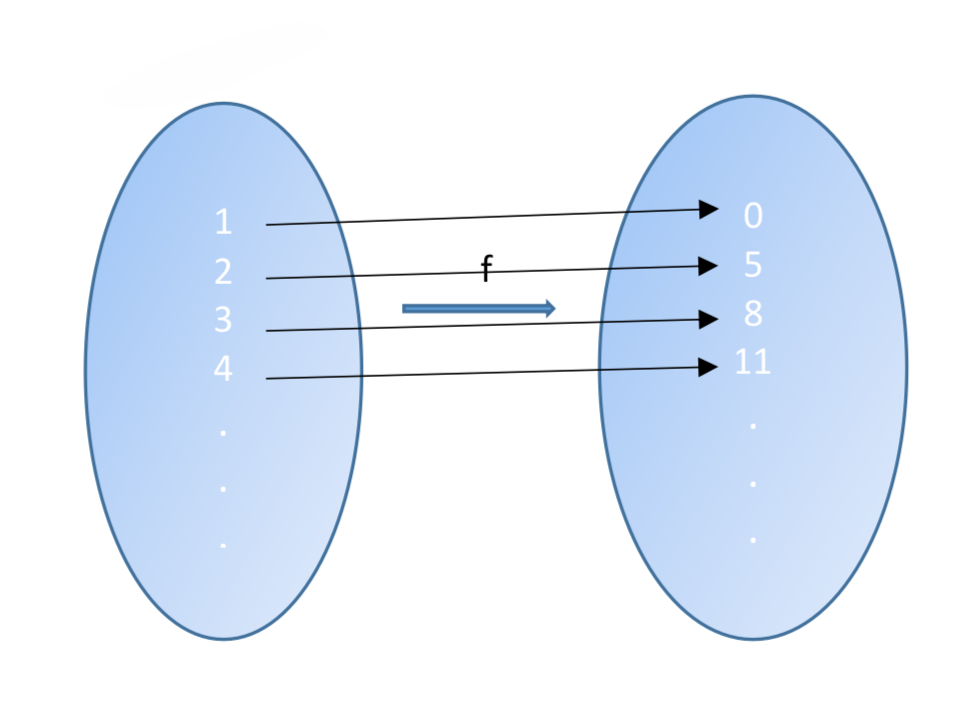
\includegraphics[width=0.3\linewidth]{IMG_1714.jpeg}
        \end{figure}
        Sí es función.
        
        \begin{enumerate}
            \item[i)] Inyectiva: Supongamos, por el contrario, sea \(a \neq b\). Si \(a=2\), \(b=3\). P.D. \(f(a) \neq f(b)\). Y como para todo elemento en el dominio le corresponde un único elemento en el codominio (como se muestra en la imagen).
            
            \(f(a) \neq f(b)\)
            \vspace{\baselineskip}
            
            Por lo tanto, \(f\) es inyectiva.

            \item[ii)] Sobre: Sí, porque en la imagen se nos muestra que en el codominio no sobran elementos.

            \item[iii)] Biyectiva: Sí, porque es suprayectiva e inyectiva.

            \item[iv)] ¿Tiene inversa? Sí, porque es biyectiva.

            \item[v)] No se pueden definir las fórmulas.
        \end{enumerate}
        \item[b)]
        \begin{figure}[H]
            \centering
            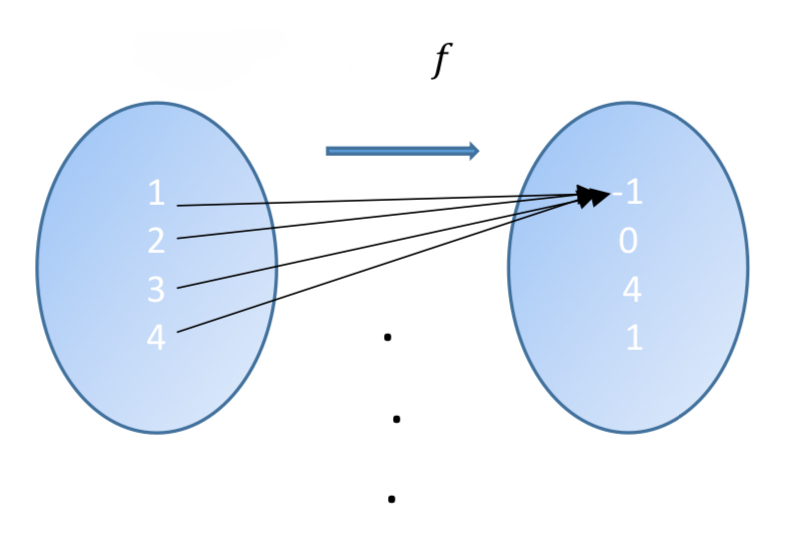
\includegraphics[width=0.3\linewidth]{IMG_1715.jpeg}
        \end{figure}
        Sí es función.

        \begin{enumerate}
            \item[i)] Inyectiva: Sea \(a \neq b\). Sea \(a = 1\) y \(b = 2\). P.D. \(f(a) \neq f(b)\)
            
            \[f(a) = -1\]
            
            \[f(b) = -1\]
            \vspace{\baselineskip}
            
            \(\Rightarrow f(a) = f(b)\)
            \vspace{\baselineskip}
            Por tanto, \(f\) no es inyectiva.

            \item[ii)] Sobre: Supongamos que es suprayectiva. Sea \(y = 4\). P.D. \(\exists x \in A\) tal que \(f(x) = y\)
            
            \(\Rightarrow -1 = 4\) \quad \textbf{CONTRADICCIÓN}
            \vspace{\baselineskip}
            
            Por lo tanto, \(f\) no es suprayectiva.

            \item[iii)] Biyectiva: No, porque no es ni inyectiva ni suprayectiva.

            \item[iv)] No tiene función inversa porque no es biyectiva.

            \item[v)] No tiene función inversa
        \end{enumerate}
        \item[c)]
        \begin{figure}[H]
            \centering
            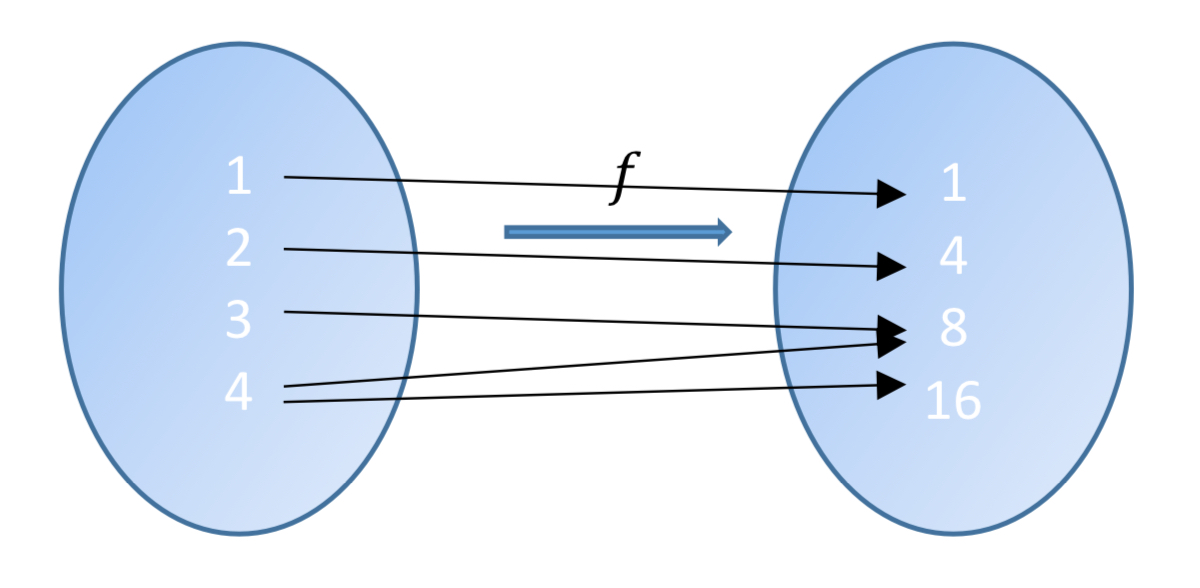
\includegraphics[width=0.3\linewidth]{IMG_1716.jpeg}
        \end{figure}
        No es función porque a un elemento del dominio le corresponden dos elementos del codominio.
        \item[d)] \(f:A\subset\mathbb{R}\rightarrow B\subset\mathbb{R}\) definida por \(f(x)=\sqrt{\frac{x-3}{6x+2}}\)

        Sí es función.
        \vspace{\baselineskip}
        
        \begin{enumerate}
            \item[i)] Inyectiva: Sea \(f(a) = f(b)\). P.D. \(a = b\)
            
            \(\frac{a - 3}{6a + 2} = \frac{b - 3}{6b + 2}\)
            
            \(\Rightarrow \frac{6b + 2}{a - 3} = \frac{b - 3}{6a + 2}\)
            
            \(\Rightarrow 6ab - 18b + 2a - 6 = 6ab + 2b - 18a - 6\)
            
            \(\Rightarrow -18b + 2a = 2b - 18a\)
            
            \(\Rightarrow \frac{20a}{20} = \frac{20b}{20}\)
            
            \(\Rightarrow a = b\)
            
            Por lo tanto, \(f\) es inyectiva.

            \item[ii)] Sobre: Sea \(y \in B\), P.D. \(\exists x \in A\) tal que \(f(x) = y\)
            
            \(y = \frac{x + 3}{6x + 2}\)
            
            \(\Rightarrow 6xy + 2y = x - 3\)
            
            \(\Rightarrow 6xy - x = -2y - 3\)
            
            \(\Rightarrow x(6y - 1) = -2y - 3\)
            
            \(\Rightarrow x = \frac{-2y - 3}{6y - 1}\)
            
            \(\Rightarrow f(x) = \frac{-2x - 3}{6x - 1}\)
            
            \(\Rightarrow f(x) = \left(\frac{-2y - 3}{6y - 1}\right)(6y - 1)\)
            
            \(\Rightarrow f(x) = \frac{-2x}{-2} - 3\)
            
            \(\Rightarrow f(x) = x - 3\)
            
            \(\Rightarrow f(x) = y - 3 + 3\)
            
            \(\Rightarrow f(x) = y\)

            Por tanto, \(f\) es suprayectiva.
            
            \item[iii)] Biyectiva: Es biyectiva porque es inyectiva y suprayectiva.

            \item[iv)] Sí tiene porque es biyectiva.

            \item[v)] \(f(x) = \frac{x - 3}{6x + 2} \quad f^{-1}(x) = \frac{-2x - 3}{6x - 1}\)
        \end{enumerate}
        \item[e)] \(f:A\subset\mathbb{R}\rightarrow B\subset\mathbb{R}\) definida por \(f(x)=\frac{-2x+5}{3x+1}\)

        Sí es función.
        \vspace{\baselineskip}
        
        \begin{enumerate}
            \item[i)] Inyectiva: Sea \(f(a) = f(b)\). P.D. \(a = b\)
            
            \(\frac{-2a + 5}{3a + 1} = \frac{-2b + 5}{3b + 1}\)
            
            \(\Rightarrow (-2a + 5)(3b + 1) = (-2b + 5)(3a + 1)\)
            
            \(\Rightarrow -6ab - 2a + 15b + 5 = -6ab - 2b + 15a + 5\)
            
            \(\Rightarrow -2a + 15b = -2b + 15a\)
            
            \(\Rightarrow 17b = 17a\)
            
            \(\Rightarrow a = b\)
            
            \(f(x)\) es inyectiva.
            
            \item[ii)] Sobre: Sea \(y \in B\), P.D. \(\exists x \in A\) tal que \(f(x) = y\)
            
            \(y = \frac{-2x + 5}{3x + 1}\)
            
            \(\Rightarrow 3xy + y = -2x + 5\)
            
            \(\Rightarrow 3xy + 2x = -y + 5\)
            
            \(\Rightarrow x(3y + 2) = -y + 5\)
            
            \(\Rightarrow x = \frac{-y + 5}{3y + 2}\)
            
            \(\Rightarrow f(x) = \frac{-x + 5}{3x + 2}\)
            
            \(\Rightarrow f(x) = \left(\frac{-x + 5}{3y + 2}\right)(3y + 2)\)
            
            \(\Rightarrow f(x) = -y + 5 - 5\)
            
            \(\Rightarrow f(x) = -y\)
            
            \(\Rightarrow f(x) = y\)
            
            Por lo tanto, \(f(x)\) es suprayectiva.
            
            \item[iii)] Biyectiva: Sí, porque es inyectiva y suprayectiva.
            
            \item[iv)] Sí, porque es biyectiva.
            
            \item[v)] \(f(x) = \frac{-2x + 5}{3x + 1}\) \quad \(g(x) = \frac{-x + 5}{3x + 2}\)
        \end{enumerate}
    \end{enumerate}
    \vspace{\baselineskip}

   \item[30.]¿Cuál de las siguientes ecuaciones son funciones? Justifique su respuesta.
   \begin{enumerate}
    \item[a)] \(y = x^2 - 2\)
    
    Es una función en \(x\), \(y(x)\), puesto que a cada valor de \(x\) sólo le corresponde un solo cuadrado al que siempre se le puede restar 2.
    \vspace{\baselineskip}
    \item[b)] $x = 2$

    Sea esta relación un subconjunto de \(\mathbb{R} \times \mathbb{R}\), tal que \(\{(x, y) \,|\, x = 2\}\), lo podemos visualizar de la siguiente manera:
    \begin{figure}[H]
        \centering
        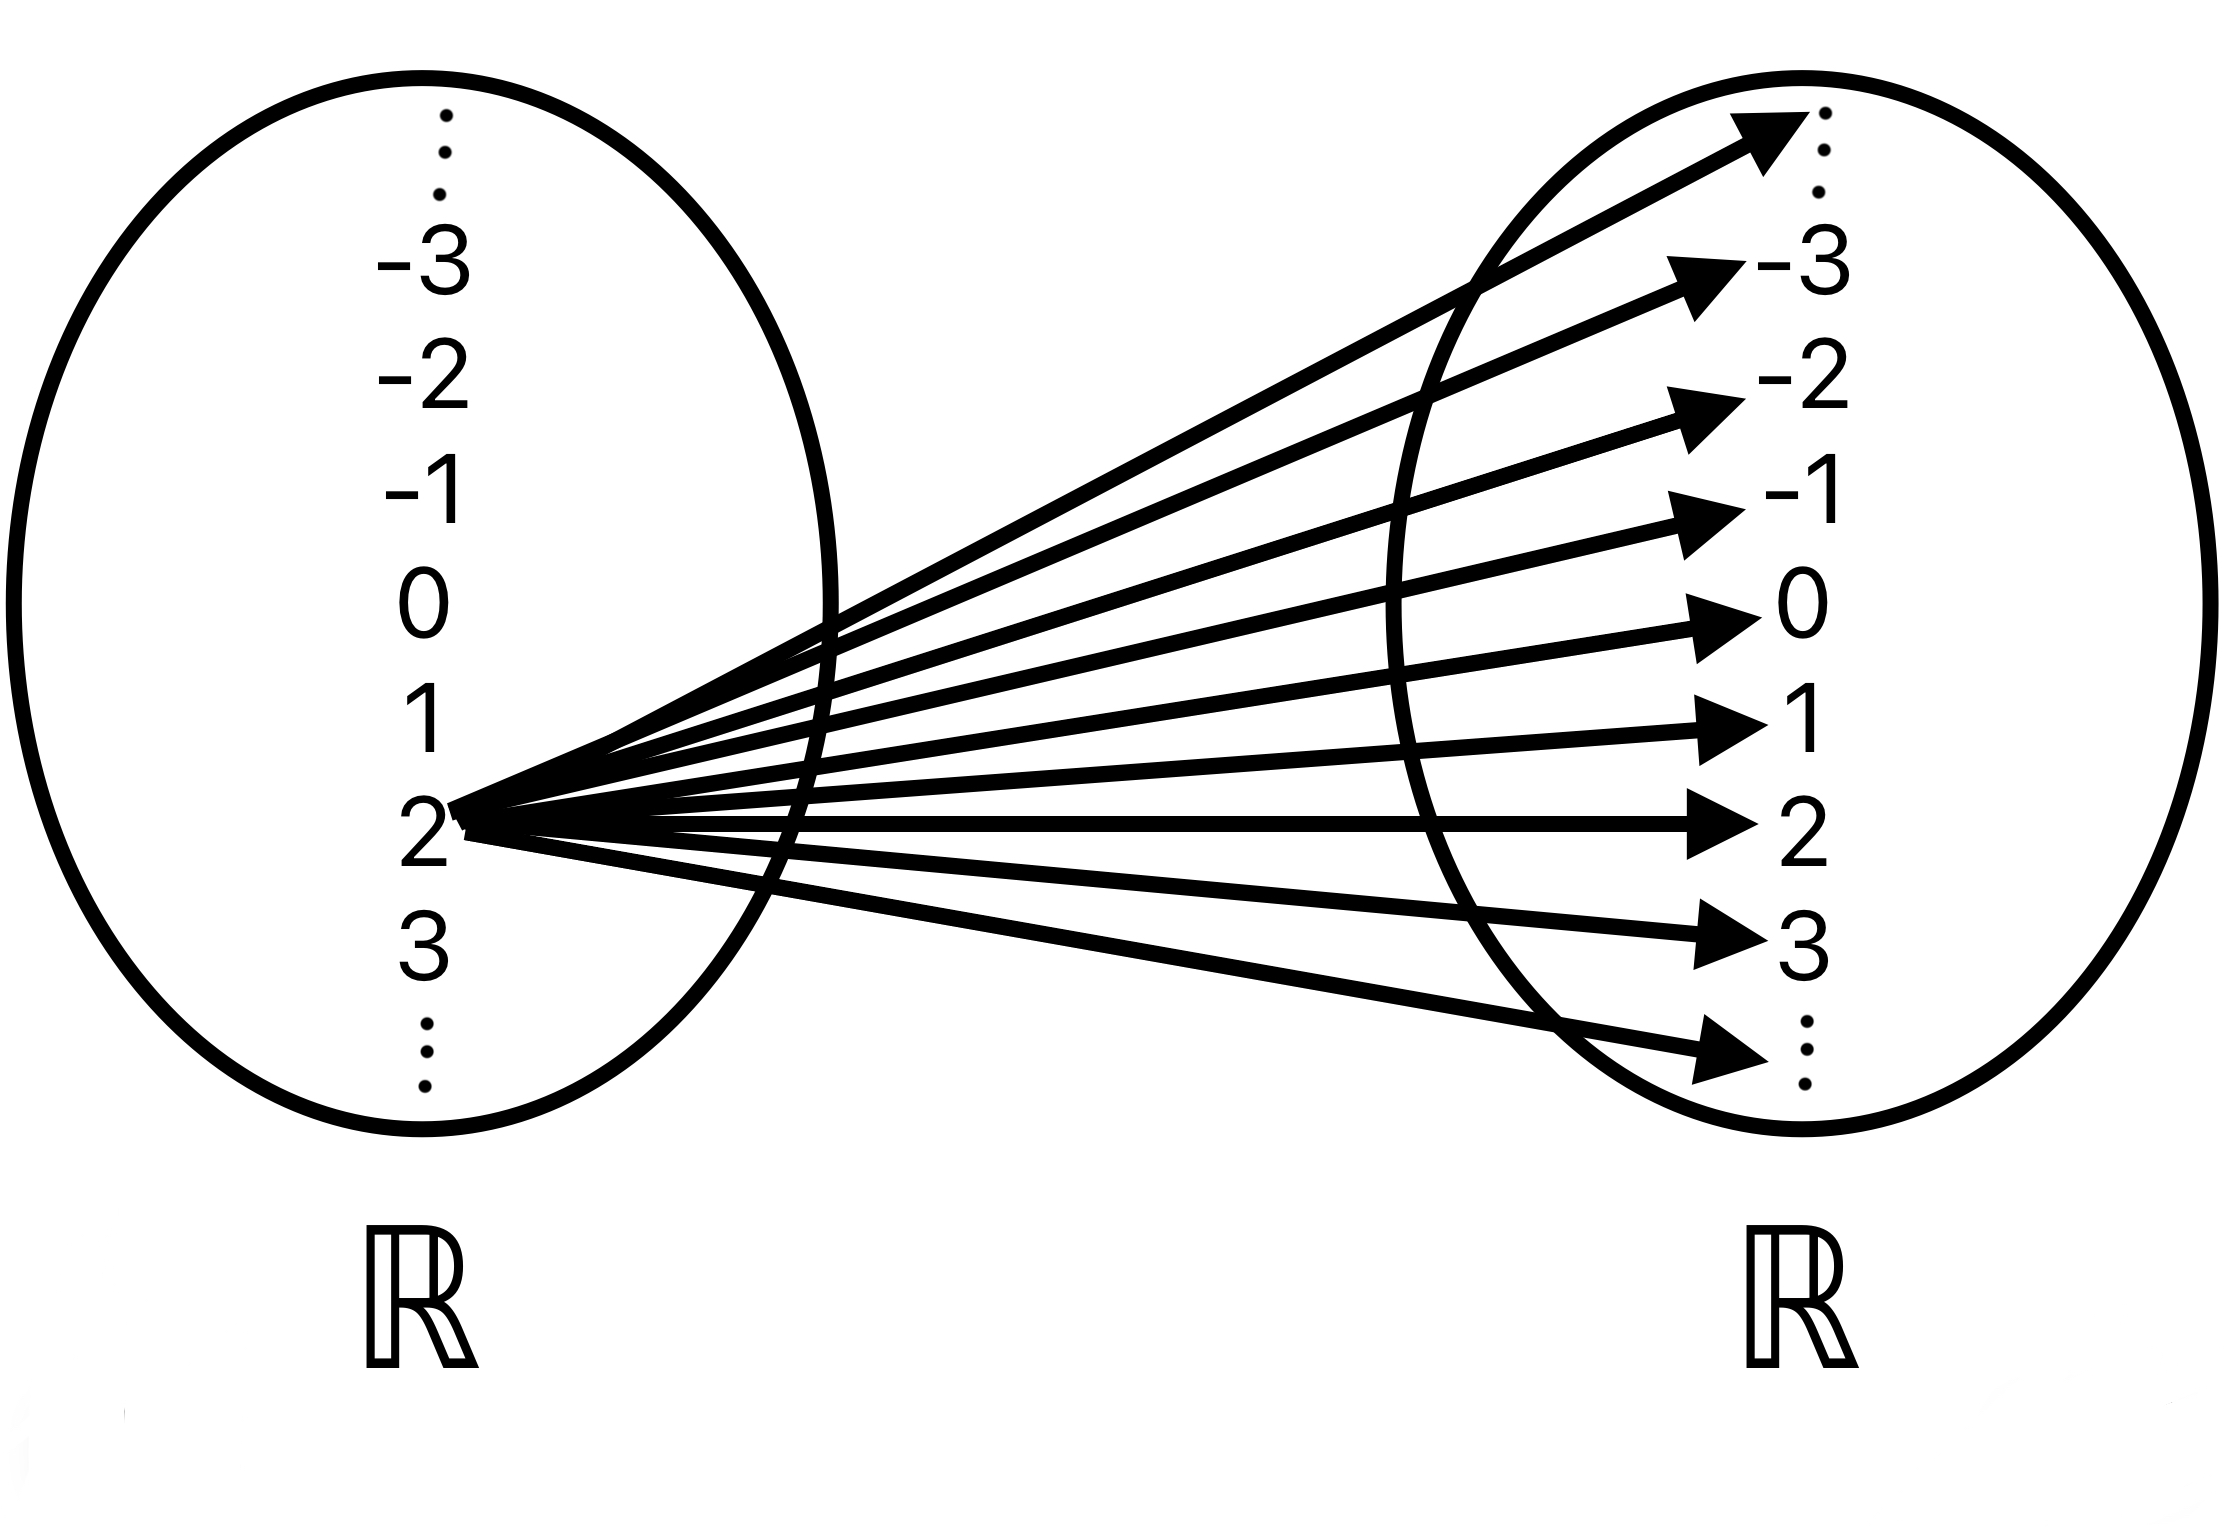
\includegraphics[width=0.3\linewidth]{IMG_1709.jpeg}
    \end{figure}
    Así, vemos que no cumple con las dos propiedades de una función: que a todo elemento del dominio le corresponda un elemento del contradominio; incluso si restringiéramos el dominio a solo \(\{2\}\), no cumple con la segunda propiedad de que a cada elemento del dominio le debe corresponder un solo elemento del contradominio.
    \vspace{\baselineskip}
    \item[c)] $y = -2x + 7$

    Es una función en \(x\), \(y(x)\), puesto que a cada valor de \(x\) solo le corresponde un único valor al multiplicar por -2 y sumarle 7.
    \vspace{\baselineskip}
    \item[d)] $y^2 = x$

    Sea esta relación un subconjunto de \(\mathbb{R} \times \mathbb{R}\), tal que \(\{(x, y) \,|\, y^2 = x\}\). Se puede plantear el contraejemplo \((1,1)\) y \((1,-1)\) que pertenecen a esta relación, y notamos que ambas parejas ordenadas tienen el mismo elemento del dominio pero dos diferentes del codominio. Por lo tanto, no es una función.
    \vspace{\baselineskip}
    \item[e)] $y = 1$

    Sea esta relación un subconjunto de \(\mathbb{R} \times \mathbb{R}\), tal que \(\{(x, y) \,|\, y = 1\}\). La podemos ilustrar como:
    \begin{figure}[H]
        \centering
        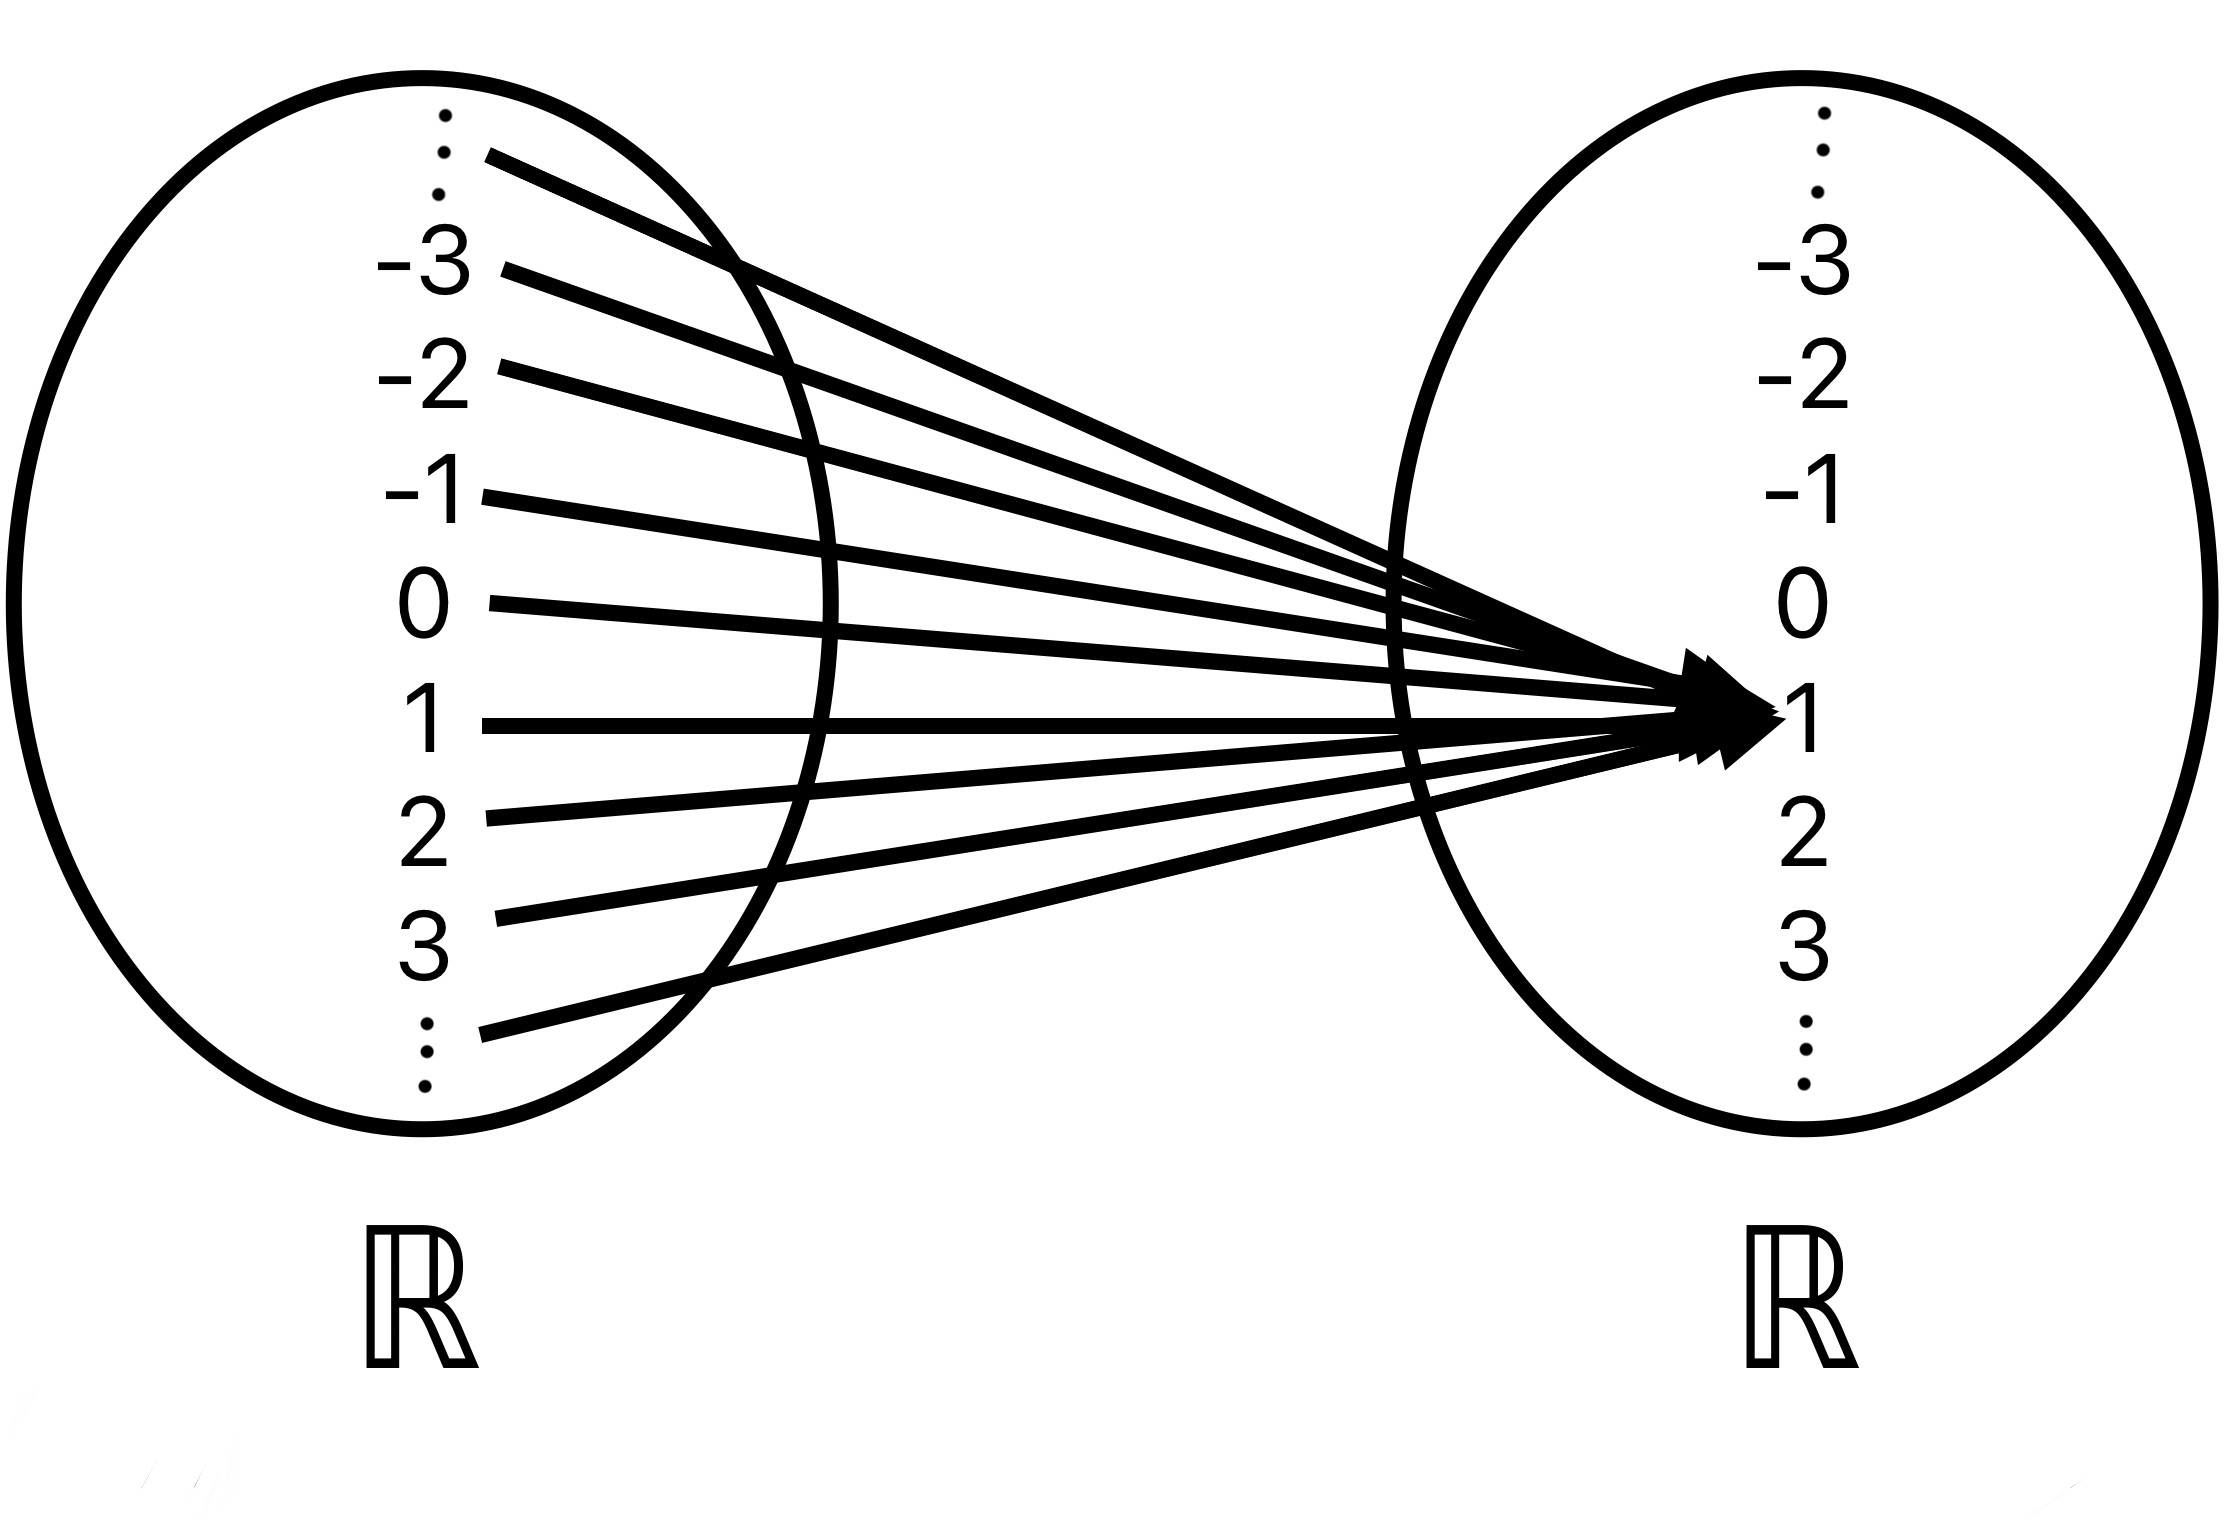
\includegraphics[width=0.3\linewidth]{IMG_1710.jpeg}
    \end{figure}
    Vemos que todos los elementos del conjunto \(\mathbb{R}\) dominio se corresponden, cada uno, con un solo valor del conjunto \(\mathbb{R}\) codominio; por tanto, es una función.
\end{enumerate}
\item[31.]Calcule el dominio y rango de las siguientes funciones.
    \begin{enumerate}
        \item[a)]\(f(x) = \frac{1}{{4x - 3}}\)
        
        Dom:
        
        $4x - 3 \neq 0$
        
        $4x \neq 3$

        $x \neq \frac{3}{4}$
        
        $Dom = \{x \in \mathbb{R} \, | \, x \neq \frac{3}{4}\} $
        
        $Dom = \mathbb{R} \setminus \left\{ \frac{3}{4} \right\}$
        \vspace{\baselineskip}

        Img:

        Dado que $4x - 3$ puede tomar cualquier valor excepto $0$ debido a la biyección de cualquier recta con $\mathbb{R}$, entonces la función puede tomar cualquier valor excepto $0$.

        $Img= \{ y \in \mathbb{R} \mid y \neq 0 \}$
        
        $Img = \mathbb{R} \setminus \{0\}$
        \vspace{\baselineskip}
        \item[b)]\(f(x) = \frac{\sqrt{x+2}}{x-3}\)

        Dom:
        
        $x - 3 \neq 0 \land x + 2 \geq 0$

        $x \neq 3 \land x \geq -2$

        $x \in (-\infty, 3) \cup (3, \infty) \land x \in [-2, \infty)$

        $x \in \left( (-\infty, 3) \cup (3, \infty) \right) \cap [-2, \infty)$

        $x \in [-2, 3) \cup (3, \infty)$
        \vspace{\baselineskip}

        $Dom = \{x \in \mathbb{R} \, | \, -2 \leq x < 3 \, \lor \, x > 3\}$

        $Dom = [-2, 3) \cup (3, \infty)$
        \vspace{\baselineskip}
        
        Img:

        Obs. $\sqrt{x+2}$ siempre es positivo o 0, y siempre es creciente.
        \vspace{\baselineskip}

Primeramente, el intervalo $x \in [-2,3)$ tiene $x-3$ negativo siempre; en -2, la función vale cero y a medida que $x-3$ se hace más negativo, la función se acerca a $-\infty$ cuando $x$ se acerca a 3. Así, al intervalo $x \in [-2,3)$ le corresponden todos los números negativos y el 0.
\vspace{\baselineskip}

En segundo lugar, el intervalo $x \in (3,\infty)$. Cuando nos acercamos a 3 por la derecha, obtenemos valores en $x-3$ muy cercanos a 0 por la derecha, por lo tanto, la función arrojará valores muy grandes. Mientras $x$ tiende al infinito, $x-3$ arroja los valores más grandes, lo que se traduce en que la función arrojará valores más cercanos a 0. Así, el intervalo $x \in (3,\infty)$ corresponde con todos los números positivos.
\vspace{\baselineskip}

Uniendo los conjuntos, la imagen de $f$ son todos los números reales $y \in \mathbb{R}$.

$Img = \{y \, | \, y \in \mathbb{R}\}$

$Img = \mathbb{R}$
        \vspace{\baselineskip}
        \item[c)]\(f(x) = \frac{\sqrt{x-2}}{x^2-4}\)

        Dom:

        $x^2 - 4\neq 0 \land x - 2\geq 0$
        
        $x^2 \neq 4 \land x \geq 2$
        
        $\lvert x \rvert \neq 2 \land x \in [2, \infty)$

        $x \neq 2 \land x \neq -2 \land x \in [2, \infty)$

        $x \in (2, \infty)$
        \vspace{\baselineskip}

        $Dom = \{x \in \mathbb{R} \, | \, x > 2\}$

        $Dom = (2, \infty)$
        \vspace{\baselineskip}
        
        Img:
        
        Obs. $\sqrt{x-2}$ siempre es creciente y positiva; nunca 0.
        \vspace{\baselineskip}
        
        Cuando $x$ se acerca a 2 por la derecha, $x^2 - 4$ se hace más pequeño, porque la diferencia se acerca a 0; esto resulta en que la función se acerca a $\infty$. Mientras $x$ se acerca a infinito, $x^2 - 4$ se hace más grande, lo que se traduce en que la función se acerca a 0. La función nunca es negativa, porque el signo solo se daría por $x^2 - 4$, pero para que $x^2 - 4$ sea negativo, se deberá evaluar $x < 2$, lo cual no está en el dominio.
        \vspace{\baselineskip}
        
        Así, la imagen son todos los reales positivos.

        $Img = \{y \in \mathbb{R} \, | \, y > 0\}$

        $Img = (0, \infty)$
        \vspace{\baselineskip}
        \item[d)]\(f(x) = \frac{x^2 + x - 2}{x^2 - x - 2}\)

        Dom:

        $x^2 - x - 2 \neq 0$

        $x^2 - x + \frac{1}{4} \neq 2 + \frac{1}{4}$

        $(x - \frac{1}{2})^2 \neq \frac{9}{4}$

        $\lvert x - \frac{1}{2} \rvert \neq \frac{3}{2}$
        \vspace{\baselineskip}

        \begin{multicols}{2}
         \begin{enumerate}
         \item[1.] Caso 1
         
         $x - \frac{1}{2} \geq 0$

         $x \geq \frac{1}{2}$

         $x \in \left[ \frac{1}{2}, \infty \right)$
         \vspace{\baselineskip}
         
         $\Rightarrow x - \frac{1}{2} \neq \frac{3}{2}$

         $x \neq 2$

         $x \in (-\infty, 2) \cup (2, \infty)$
         \vspace{\baselineskip}
         
         $\Rightarrow x \in \left( (-\infty, 2) \cup (2, \infty) \right) \cap \left[ \frac{1}{2}, \infty \right)$

         $x \in \left[ \frac{1}{2}, 2 \right) \cup (2, \infty)$
         \vspace{\baselineskip}
         
         \item[2.] Caso 2

         $x - \frac{1}{2} < 0$

         $x < \frac{1}{2}$

         $x \in (-\infty, \frac{1}{2})$
         \vspace{\baselineskip}

         $\Rightarrow -(x - \frac{1}{2}) \neq \frac{3}{2}$

         $-x + \frac{1}{2} \neq \frac{3}{2}$

         $x \neq -1$

         $x \in (-\infty, -1) \cup (-1, \infty)$
         \vspace{\baselineskip}
         
         $\Rightarrow x \in \left( (-\infty, -1) \cup (-1, \infty) \right) \cap (-\infty, \frac{1}{2})$

         $x \in (-\infty, -1) \cup (-1, \frac{1}{2})$
         \end{enumerate}
         \end{multicols}
         \vspace{\baselineskip}
         
         $x \in \left( \left[ \frac{1}{2}, 2 \right) \cup \left( 2, \infty \right) \right) \cup \left( \left( -\infty, -1 \right) \cup \left( -1, \frac{1}{2} \right) \right)$

         $x \in \mathbb{R} \setminus \{-1, 2\}$
         \vspace{\baselineskip}

         $Dom = \{x \in \mathbb{R} \, | \, x \neq -1 \land x \neq 2\}$
         
         $Dom = \mathbb{R} \setminus \{-1, 2\}$
         \vspace{\baselineskip}

         Img:
         
         Primero, calculemos en qué intervalos las dos funciones son positivas y negativas, así como sus raíces.
          \begin{enumerate}
              \item[1.]$x^2 + x - 2$
              \vspace{\baselineskip}

              $x^2 + x - 2 > 0$

              $x^2 + x + \frac{1}{4} > 2 + \frac{1}{4}$
              
              $(x + \frac{1}{2})^2 > \frac{9}{4}$

              $\lvert x + \frac{1}{2} \rvert > \frac{3}{2}$

              \begin{multicols}{2}
              Caso 1
              
              $x + \frac{1}{2} \geq 0$

              $x \geq -\frac{1}{2}$

              $x \in [-\frac{1}{2}, \infty)$
              \vspace{\baselineskip}

              $\Rightarrow x + \frac{1}{2} > \frac{3}{2}$

              $x > 1$

              $x \in (1, \infty)$
              \vspace{\baselineskip}
              
              $\Rightarrow x\in(1,\infty)\cap[-\frac{1}{2},\infty)$

              $x \in (1, \infty)$
              \vspace{\baselineskip}

              Caso 2

              $x + \frac{1}{2} < 0$

              $x < -\frac{1}{2}$

              $x \in (-\infty, -\frac{1}{2})$
              \vspace{\baselineskip}
              
              $\Rightarrow -(x + \frac{1}{2}) > \frac{3}{2}$

              $-x - \frac{1}{2} > \frac{3}{2}$

              $x < -2$

              $x \in (-\infty, -2)$
              \vspace{\baselineskip}
              
              $\Rightarrow x \in (-\infty, -2) \cap (-\infty, -\frac{1}{2})$

              $x \in (-\infty, -2)$
              \end{multicols}
              Así, \(x^2+x-2\) es positiva en:

              $x \in (-\infty, -2) \cup (1, \infty)$
              \vspace{\baselineskip}
              
              Lógicamente, es negativa en su complemento menos sus raíces:

              $x \in (-2, 1)$
              \vspace{\baselineskip}

              Y vale $0$ en:

              $x \in \{-2, 1\}$

              \item[2.]$x^2 - x - 2$
              \vspace{\baselineskip}
              
              $x^2 - x - 2 > 0$

              $x^2 - x + \frac{1}{4} > 2 + \frac{1}{4}$

              $(x - \frac{1}{2})^2 > \frac{9}{4}$

              $\lvert x - \frac{1}{2}\rvert > \frac{3}{2}$

              \begin{multicols}{2}
              Caso 1
              
              $x - \frac{1}{2} \geq 0$

              $x \geq \frac{1}{2}$

              $x \in \left[ \frac{1}{2}, \infty \right)$
              \vspace{\baselineskip}

              $\Rightarrow x - \frac{1}{2} > \frac{3}{2}$

              $x > 2$

              $x \in (2, \infty)$
              \vspace{\baselineskip}

              $\Rightarrow x \in (2, \infty) \cap \left[ \frac{1}{2}, \infty \right)$

              $x \in (2, \infty)$
              \vspace{\baselineskip}

              Caso 2

              $x - \frac{1}{2} < 0$

              $x < \frac{1}{2}$

              $x \in (-\infty, \frac{1}{2})$
              \vspace{\baselineskip}
              
              $\Rightarrow -(x - \frac{1}{2}) > \frac{3}{2}$

              $-x + \frac{1}{2} > \frac{3}{2}$

              $x < -1$

              $x \in (-\infty, -1)$
              \vspace{\baselineskip}

              $\Rightarrow x \in (-\infty, -1) \cap (-\infty, \frac{1}{2})$

              $x \in (-\infty, -1)$
              \end{multicols}
              Así, $x^2 - x - 3$ es positiva en:

              $x \in (-\infty, -1) \cup (2, \infty)$
              \vspace{\baselineskip}

              Es negativa en:

              $x \in (-1, 2)$
              \vspace{\baselineskip}

              Y vale $0$ en:

              $x \in \{-1, 2\}$
          \end{enumerate}
          \vspace{\baselineskip}
          
         Resumiendo:
            \begin{itemize}
            \item $x \in (-\infty, -2) \cup (1, \infty) \Rightarrow x^2 + x - 2 > 0$
            \item $x \in (-2, 1) \Rightarrow x^2 + x - 2 < 0$
            \item $x = -2 \lor x = 1 \Rightarrow x^2 + x - 2 = 0$
            \end{itemize}
        \vspace{\baselineskip}
            \begin{itemize}
                \item $x \in (-\infty, -1) \cup (2, \infty) \Rightarrow x^2 - x - 2 > 0$
                \item $x \in (-1, 2) \Rightarrow x^2 - x - 2 < 0$
                \item $x = -1 \lor x = 2 \Rightarrow x^2 - x - 2 = 0$
            \end{itemize}
        \vspace{\baselineskip}

        Tomemos el segundo intervalo del dominio $x \in (-1, 2)$. Veamos qué evalúan cuando se intersecan con él:
            \begin{itemize}
                \item $\in (1, 2) \Rightarrow x^2 + x - 2 > 0$
                \item $x \in (-1, 1) \Rightarrow x^2 + x - 2 < 0$
                \item $x = 1 \Rightarrow x^2 + x - 2 = 0$
            \end{itemize}
        \vspace{\baselineskip}
            \begin{itemize}
                \item $x \in \emptyset \Rightarrow x^2 - x - 2 > 0$ (La función nunca es positiva)
                \item $x \in (-1, 2) \Rightarrow x^2 - x - 2 < 0$ (La función siempre es negativa)
                \item $x \in \emptyset \Rightarrow x^2 - x - 2 = 0$ (La función nunca es 0, pero se acerca a 0 cuando $x$ se acerca a -1 y 2)
            \end{itemize}
        \vspace{\baselineskip}
        Ya en nuestra función \(f(x)\); cuando nos acercamos por la derecha a -1, nuestro denominador siempre negativo se acerca a 0 y el numerador negativo se acerca a:
        
        $(-1)^2 + (-1) - 2 = -2$
        \vspace{\baselineskip}
        
        Por tanto, la función se acerca a \(+\infty\). Mientras \(x\) avanza hacia \(x = 1\), el denominador se acerca a -1 y el numerador a 0; por tanto, el valor de la función se acerca a 0. Finalmente, cuando \(x > 1\), la función será negativa porque el denominador siempre es negativo y el numerador positivo; cuando \(x\) se acerca a 2, el denominador se acerca a 0 y el numerador se acerca a:
        
        $(2)^2 + 2 - 2 = 4$
        \vspace{\baselineskip}
        
        Así, la función se acerca a \(-\infty\) mientras \(x\) se acerca a 2.
        \vspace{\baselineskip}
        
        Concluimos que en el intervalo \(x \in (-1,2)\), la función va de \(+\infty\) a \(-\infty\); por tanto, sin importar la imagen directa de los otros intervalos del conjunto dominio, la imagen de toda la función es \(\mathbb{R}\).
        \vspace{\baselineskip}

        $Img = \{y \,|\, y \in \mathbb{R}\}$
        
        $Img = \mathbb{R}$
        \vspace{\baselineskip}
        
        \item[e)]\(f(x) = 7 + \sqrt{3x - 6}\)

        Dom:

        $3x - 6 \geq 0$

        $3x \geq 6$

        $x \geq 2$
        \vspace{\baselineskip}

        $Dom = \{x \in \mathbb{R} | x \geq 2\}$

        $Dom = [2, \infty)$
        \vspace{\baselineskip}

        Img:
        
        Como sabemos que la función raíz siempre es creciente, evaluamos en el primer valor del dominio y deducimos que todos los valores mayores a él estarán en la imagen de \(f\).
        \vspace{\baselineskip}

        $f(2) = 7 + \sqrt{3 \cdot 2 - 6}$

        $f(2) = 7$
        \vspace{\baselineskip}

        $\Rightarrow Img = \{y \in \mathbb{R} \mid y \geq 7\}$

        $Img = [7, \infty)$
        \vspace{\baselineskip}
        
        \item[f)]\(f(x) = \frac{\sqrt{-x+1}}{\sqrt{x^2-1}}\)

        Dom:

        $-x + 1 \geq 0 \land x^2 - 1 > 0$

        $x \leq 1 \land x^2 > 1$

        $x \in (-\infty, 1] \land \lvert x \rvert > 1$

        $x \in (-\infty, 1] \land (x > 1 \land x < -1)$

        $x \in (-\infty, 1] \land x \in (-\infty, -1) \cup (1, \infty)$

        $x \in (-\infty, 1] \cap ((-\infty, -1) \cup (1, \infty))$

        $x \in (-\infty, -1)$
        \vspace{\baselineskip}

        $Dom = \{x \in \mathbb{R} | x < -1\}$

        $Dom = (-\infty, -1)$
        \vspace{\baselineskip}

        Img:

        Dado que tanto el numerador como el denominador son raíces, toda la función siempre será positiva. Además, dado que el valor de cero de la función \(\sqrt{-x+1}\) no existe en el dominio de \(f\), la función nunca vale cero.
        \vspace{\baselineskip}
        
        Cuando \(x\) es un número negativo muy grande, es decir, cuando se acerca a \(-\infty\), \(-x+1\) será forzosamente más pequeño que \(x^2-1\) y, por extensión, sus raíces también; así, el denominador se hace más grande más rápidamente que el numerador, por tanto se acerca a 0.
        \vspace{\baselineskip}
        
        Ahora, cuando \(x\) se acerca a \(-1\) por la izquierda, el numerador se acerca a:
        
        $-(-1)+1 = 2$
        \vspace{\baselineskip}
        
        Y el denominador se acerca a 0; esto resulta en que la función se acerque a \(+\infty\).
        \vspace{\baselineskip}
        
        Por tanto, la función toma valores de 0 a \(\infty\).
        \vspace{\baselineskip}
        
        $Img = \{y \in \mathbb{R} \mid y > 0\}$
        
        $Img = (0, \infty)$
\end{enumerate}

\item[32.] Demuestra si las  funciones son inyectivas, sobreyectivas o biyectivas. Si la función es biyectiva, encuentre su inversa.
    \begin{enumerate}
        \item[a)] \(f: \mathbb{N} \rightarrow \mathbb{N} \text{ con } f(x) = x + 1\)
            \begin{enumerate}
                \item[1.] P.D. \(f\) es inyectiva.
                    
                    $\Rightarrow \forall a, b \in \mathbb{N}, \, f(a) = f(b) \, \text{implica} \, a = b$
                    \begin{proof}
                        Sean \(a, b \in \mathbb{N}\), supongamos que \(f(a) = f(b)\), por definición:

                        $f(a) = a + 1$

                        $f(b) = b + 1$
                        \vspace{\baselineskip}

                        $\Rightarrow a + 1 = b + 1$

                        $a + 1 - 1 = b + 1 - 1$

                        $a = b$
                    \end{proof}
                \item[2.] P.D. \(f\) no es suprayectiva.

                    $\Rightarrow \neg (\forall b \in \mathbb{N}, \exists a \in \mathbb{N} \text{ tal que } f(a) = b)$
                    
                    $\Rightarrow \exists b \in \mathbb{N} \text{ tal que } \forall a \in \mathbb{N}, f(a) \neq b$
                    \vspace{\baselineskip}
                    
                    \begin{proof}
                        Sea \(b = 1\), P.D. \(\forall a \in \mathbb{N} \), \( f(a) \neq 1 \)
                        \vspace{\baselineskip}
                        
                        Por inducción matemática, llámese esta propiedad \(p(a)\), \(\forall a \in \mathbb{N}\)
                        \begin{enumerate}
                            \item[1.] Caso básico
                        
                                \(p(1):\)

                                \(f(1) \neq 1\)

                                \(1 + 1 \neq 1\)

                                \(2 \neq 1\)

                                Correcto
                                \vspace{\baselineskip}
                                
                            \item[2.] Paso inductivo
                            
                                p(k): \( f(k) \neq 1 \)
                            
                                \(\Rightarrow k+1 \neq 1 \) \textbf{HIPÓTESIS DE INDUCCIÓN}
                                \vspace{\baselineskip}

                                p(k+1): \(f(k + 1) \neq 1\)
                            
                                \(\Rightarrow (k + 1) + 1 \neq 1\) \textbf{P.D.}
                                \vspace{\baselineskip}

                                La hipótesis dicta que \( k+1 \neq 1 \), por tanto, por axiomas de orden:

                                \( k+1 > 1  \lor  k+1 < 1\)
                                
                                \( k+1 > 1 \lor k < 0 \)
                                \vspace{\baselineskip}

                                Aquí, el segundo caso es imposible porque \( k \in \mathbb{N} \). Tomemos el caso válido.
                                \vspace{\baselineskip}
                                
                                Por otro lado, es evidente que:
                                
                                \( k+2 > k+1 \)
                                \vspace{\baselineskip}
                                
                                Y, en el caso válido, por transitividad:
                                
                                \( k+2 > k+1 > 1 \)
                                
                                \( k+2 > 1 \)
                                \vspace{\baselineskip}
                                
                                Como todo número \( k+2 \) mayor estricto a $1$ implica que es diferente a $1$, entonces:
                                
                                \( k+2 \neq 1 \)

                                \((k + 1) + 1 \neq 1\)
                                \vspace{\baselineskip}
                                
                                Por hipótesis de inducción, la propiedad \( p(a) \) se cumple para toda \( a \in \mathbb{N} \); y por extensión, la función no es suprayectiva, porque existe el valor \( b = 1 \) que no se puede alcanzar con ningún valor de \( a \in \mathbb{N} \).
                    \end{enumerate}
                    \end{proof}
                \item[3.] Como \(f\) no es suprayectiva, entonces no es biyectiva.
                \item[4.] Como \(f\) no es biyectiva, entonces no tiene función inversa.
            \end{enumerate}
            \vspace{\baselineskip}
            
        \item[b)] \( f: \mathbb{R} \setminus \left\{-\frac{3}{7}\right\} \rightarrow \mathbb{R} \setminus \left\{\frac{2}{7}\right\} \text{ con } f(x) = \frac{2x-7}{7x+3} \)
            \begin{enumerate}
            \item[1.] P.D. \( f \) es inyectiva.
                \(\Rightarrow \forall a, b \in \mathbb{R} \setminus \left\{-\frac{3}{7}\right\}, f(a) = f(b) \) implica \( a = b \)
                
                \begin{proof} Sean \( a, b \in \mathbb{R} \setminus \left\{-\frac{3}{7}\right\} \), supongamos que \( f(a) = f(b) \), por definición de \(f(x)\):
                
                \( f(a) = \frac{2a - 7}{7a + 3} \)
                
                \( f(b) = \frac{2b - 7}{7b + 3} \)
                \vspace{\baselineskip}
                
                \(\Rightarrow \frac{2a - 7}{7a + 3} = \frac{2b - 7}{7b + 3} \)
                
                \((7b + 3)(2a - 7) = (2b - 7)(7a + 3) \)
                
                \(14ab - 49b + 6a - 21 = 14ab + 6b - 49a - 21 \)
                
                \(6a + 49a = 6b + 49b \)
                
                \(55a = 55b \)
                
                \(a = b \)
                
                \end{proof}
            \item[2.] P.D. \( f \) es suprayectiva.
                
                \(\Rightarrow \forall b \in \mathbb{R} \setminus \left\{\frac{2}{7}\right\}, \exists a \in \mathbb{R} \setminus \left\{-\frac{3}{7}\right\} \) tal que \( f(a) = b \)
                
                \begin{proof} Sea \( b \in \mathbb{R} \setminus \left\{\frac{2}{7}\right\} \) (es decir, \( b \neq \frac{2}{7} \)), supongamos que \( a = \frac{3b + 7}{2 - 7b} \). Como \( b \neq \frac{2}{7} \), entonces \( 2 - 7b \) nunca vale \( 0 \) y es válido despejar.
                
                \( a(2 - 7b) = 3b + 7 \)
                
                \( 2a - 7ab = 3b + 7 \)
                
                \( 3b + 7ab = 2a - 7 \)
                
                \( b(3 + 7a) = 2a - 7 \)
                \vspace{\baselineskip}
                
                Supongamos que \( a \neq -\frac{3}{7} \) para que \( 7a + 3 \) sea diferente de \( 0 \) y se pueda dividir de ambos lados:
                
                \( b = \frac{2a - 7}{7a + 3} \)
                \vspace{\baselineskip}
                
                Por definición de \( f \), esta expresión es igual a \( f(a) \):
                
                \( b = f(a) \)
                \vspace{\baselineskip}
                
                Hemos demostrado que cualquier \( b \neq \frac{2}{7} \) puede ser obtenida de alguna \( a \neq -\frac{3}{7} \) (que toma la forma específica \( \frac{3b + 7}{2 - 7b} \)) evaluada en \( f \).
                
                \end{proof}
            \item[3.] Como \( f \) es inyectiva y suprayectiva, entonces \( f \) es biyectiva.
            
            \item[4.] Se obtiene la función inversa:
            
                \( f(x) = \frac{2x - 7}{7x + 3} \)
            
                \( y = \frac{2x - 7}{7x + 3} \)
                \vspace{\baselineskip}
                
                \(\rightarrow x = \frac{2y - 7}{7y + 3} \)
                
                \( x(7y + 3) = 2y - 7 \)
                
                \( 7xy + 3x = 2y - 7 \)
                
                \( 7xy - 2y = -7 - 3x \)
                
                \( y(2 - 7x) = 3x + 7 \)
                
                \( y = \frac{3x + 7}{2 - 7x} \)
                \vspace{\baselineskip}
                
                Como \( f \) es biyectiva, los conjuntos dominio y codominio se invierten:
                
                \( f^{-1} : \mathbb{R} \setminus \left\{\frac{2}{7}\right\} \rightarrow \mathbb{R} \setminus \left\{-\frac{3}{7}\right\} \quad \) dada por:\( \quad f^{-1}(x) = \frac{3x + 7}{2 - 7x} \)
            \end{enumerate}
            \vspace{\baselineskip}
            
        \item[c)] \(f: \mathbb{R} \rightarrow \mathbb{R}^+ \cup \{0\} \text{ con } f(x) = \lvert x \rvert\)
        
        Diremos que el codominio es \(\mathbb{R}^+ \cup \{0\}\) porque sino \(f\) no sería función (el 0 no correspondería con ningún valor).
        \begin{enumerate}
            \item[1.] P.D. \(f\) no es inyectiva.

            \(\Rightarrow \neg (\forall a, b \in \mathbb{R}, f(a) = f(b) \Rightarrow a = b)\)
            
            \(\Rightarrow \exists a, b \in \mathbb{R}, \text{tal que } f(a) = f(b) \land a \neq b\)
            \vspace{\baselineskip}

            \begin{proof} Sean \(a = -1\) y \(b = 1\), P.D. \(f(a) = f(b) \land a \neq b\).
            \begin{multicols}{2}
                \(f(a)=|-1|=1\)
                
                \(f(b)=|1|=1\)
                \vspace{\baselineskip}
                
                \(\Rightarrow f(a)=f(b)\)
                \columnbreak
                
                \(a = 1 \land b = -1\)
                \vspace{\baselineskip}
                
                \(\Rightarrow a \neq b\)
            \end{multicols}

            Así, \(f\) no es inyectiva.
            
            \end{proof}
            \item[2.] P.D. \(f\) es suprayectiva.
            
            \(\Rightarrow \forall b \in \mathbb{R}^+ \cup \{0\}, \exists a \in \mathbb{R} \text{ tal que } f(a) = b\)
            \vspace{\baselineskip}
            
            \begin{proof} Sea \(b \in \mathbb{R}^+ \cup \{0\}\) (es decir, \(b \geq 0\)), supongamos que \(a = b\), por ejemplo. Entonces:
            
            \(f(a) = \lvert a \rvert\)
            
            \(f(b) = \lvert b \rvert\)
            \vspace{\baselineskip}
            
            \(\Rightarrow f(a) = f(b)\)
            
            Así, demostramos que cualquier \(b \geq 0\) se puede obtener de alguna \(a\) que tenga la forma \(b\), evaluada en \(f\) (no es la única forma, pero sólo tenemos que exhibir que existe una que cumpla \(f(a) = b\)). Además, como \(a = b\) y \(b \in \mathbb{R}^+ \cup \{0\}\), entonces \(a \in \mathbb{R}^+ \cup \{0\}\) y \(a \in \mathbb{R}\).
            
            \end{proof}
            \item[3.] Como \(f\) no es inyectiva, entonces no es biyectiva.
            \item[4.] Como \(f\) no es biyectiva, entonces no tiene función inversa.
        \end{enumerate}
        \vspace{\baselineskip}
        
        \item[d)] \(f: \mathbb{N} \rightarrow \mathbb{N} \text{ con } f(x) = \frac{x}{3}\)

        Con el dominio dado, \( f \) no es una función, pues existe algún valor, \( 1 \) por ejemplo, que no tiene imagen en \( \mathbb{N} \); pues \( f(1) = \frac{1}{3} \notin \mathbb{N} \)
        \vspace{\baselineskip}
        
        \item[e)] \(f:\mathbb{R}\rightarrow\mathbb{R} \text{ con } f(x) = mx + c\), donde \(m\) y \(c\) son constantes
        \begin{itemize}
            \item Caso 1: \(m = 0\)

            \(\Rightarrow f(x) = 0(x) + c\)
            
            \(\Rightarrow f(x) = c\)
            \begin{enumerate}
                \item[1.] P.D. \(f\) no es inyectiva.
                
                \(\Rightarrow \neg (\forall a, b \in \mathbb{R}, f(a) = f(b) \implies a = b)\)
                
                \(\Rightarrow \exists a, b \in \mathbb{R}, f(a) = f(b) \land a \neq b\)
                
                \begin{proof} Sea \(a = 1\) y \(b = 2\), P.D \(f(a) = f(b) \land a \neq b\)
                \begin{multicols}{2}
                    \(f(a) = f(1) = c\)
                    
                    \(f(b) = f(2) = c\)
                    \vspace{\baselineskip}

                    \(\Rightarrow f(a) = f(b)\)
                    \columnbreak
                    
                    \(a = 1\) y \(b = 2\)
                    \vspace{\baselineskip}
                    
                    \(\Rightarrow a \neq b\)
                \end{multicols}

                Así, cuando \(m = 0\), \(f\) no es inyectiva.
                
                \end{proof}
                \item[2.] P.D. \(f\) no es suprayectiva.
                
                \(\Rightarrow \lnot (\forall b \in \mathbb{R}, \exists a \in \mathbb{R} \text{ tal que } f(a) = b)\)

                \(\Rightarrow \exists b \in \mathbb{R} \text{ tal que } \forall a \in \mathbb{R}, f(a) \neq b\)
                \vspace{\baselineskip}
                \begin{proof}
                Sea \(b = c + 1\), P.D. \(\forall a\in\mathbb{R}\), \(f(a) \neq b\)

                Sea una \(a\in\mathbb{R}\):
                
                \(f(a)=c\)

                \(f(a) \neq c + 1\)
                
                \(\therefore f(a) \neq b\)

                Así, cuando \(m = 0\), \(f\) no es suprayectiva.
                
                \end{proof}
                \item[3.] Cuando \(m = 0\), \(f\) no es biyectiva porque no es ni suprayectiva ni intectiva.
                \item[4.] Cuando \(m = 0\), \(f\) no es biyectiva; por lo tanto, no tiene función inversa.
            \end{enumerate}
            \item Caso 2: \(m \neq 0\)
            \begin{enumerate}
                \item[1.] P.D. \(f\) es inyectiva
                
                \(\Rightarrow \forall a,b \in \mathbb{R}, f(a) = f(b)\) implica \(a = b\)
                
                \begin{proof} Sean \(a,b \in \mathbb{R}\), supongamos \(f(a) = f(b)\):
                
                \(f(a) = ma + c\)
                
                \(f(b) = mb + c\)
                \vspace{\baselineskip}

                Así:
                
                \(f(a) = f(b)\)
                
                \(ma + c = mb + c\)
                
                \(ma + c - c = mb + c - c\)
                
                \(ma = mb\)
                \vspace{\baselineskip}
                
                Cuando \(m \neq 0\) podemos dividir ambos lados, entonces:
                
                \(a = b\)
                
                \end{proof}
                \item[2.] P.D. \(f\) es suprayectiva
                
                \(\Rightarrow \forall b \in \mathbb{R}, \exists a \in \mathbb{R}\) tal que \(f(a) = b\)
                
                \begin{proof} Sea \(b \in \mathbb{R}\), supongamos que \(a = \frac{b-c}{m}\). Como \(m \neq 0\), podemos despejar \(b\):
                
                \(a = \frac{b-c}{m}\)
                
                \(ma = b-c\)
                
                \(b = ma + c\)
                \vspace{\baselineskip}
                
                Por definición de \(f\), esto es \(f(a)\):
                
                \(f(a) = b\)
                \vspace{\baselineskip}
                
                Demostramos entonces que cualquier \(b \in \mathbb{R}\) se puede obtener de alguna \(a \in \mathbb{R}\) (que tenga la forma específica \(\frac{b-c}{m}\)) evaluada en \(f\).

                \end{proof}
                \item[3.] Cuando \(m \neq 0\), \(f\) es biyectiva porque es tanto inyectiva como suprayectiva.
                \item[4.] Como \(f\) es biyectiva, se obtiene su función inversa:
                
                \(f(x) = mx + c\)
                
                \(y = mx + c\)
                \vspace{\baselineskip}
                
                \(\rightarrow x = my + c\)
                
                \(x - c = my\)
                
                \(y = \frac{x - c}{m}\)
                \vspace{\baselineskip}
                
                Como \(f\) es biyectiva, invertimos los conjuntos dominio y codominio para \(f^{-1}\):
                
                \(f^{-1} : \mathbb{R} \rightarrow \mathbb{R}\) dada por: \(f^{-1}(x) = \frac{x - c}{m}\)
            \end{enumerate}
        \end{itemize}
    \end{enumerate}
    
\item[33.] Redefina el dominio y rango de las siguientes funciones para que sean biyectivas y halle su inversa.
    \begin{enumerate}
        \item[a)] \(f : \mathbb{R} \rightarrow \mathbb{R} \text{ con } f(x) = \frac{3x - 9}{5x - 10}\)
        
        Dom:
        
        \(5x - 10 \neq 0\)
        
        \(5x \neq 10\)
        
        \(x \neq 2\)
        
        \(x \in \mathbb{R} \setminus \{2\}\)
        
        \(x \in (-\infty, 2) \cup (2, \infty)\)
        \vspace{\baselineskip}
        
        Sacando la función inversa:
        
        \(f(x) = \frac{3x - 9}{5x - 10}\)
        
        \(y = \frac{3x - 9}{5x - 10}\)
        \vspace{\baselineskip}
        
        \(\rightarrow x = \frac{3y - 9}{5y - 10}\)
        
        \(x(5y - 10) = 3y - 9\)
        
        \(5xy - 10x = 3y - 9\)
        
        \(5xy - 3y = 10x - 9\)
        
        \(y(5x - 3) = 10x - 9\)
        
        \(y = \frac{10x - 9}{5x - 3}\)
        \vspace{\baselineskip}
        
        \(\Rightarrow f^{-1}(x) = \frac{10x - 9}{5x - 3}\)
        \vspace{\baselineskip}
        
        Con base en el dominio de la función inversa, sacamos el codominio de la función \(f\):
        
        \(5y - 3 \neq 0\)
        
        \(5y \neq 3\)
        
        \(y \neq \frac{3}{5}\)
        
        \(y \in \mathbb{R} \setminus \{\frac{3}{5}\}\)
        
        \(y \in (-\infty, \frac{3}{5}) \cup (\frac{3}{5}, \infty)\)
        \vspace{\baselineskip}
        
        Entonces la función \(f\) es:
        
        \(f : \mathbb{R} \setminus \{2\} \rightarrow \mathbb{R} \setminus \{\frac{3}{5}\}\) dada por: \(f(x) = \frac{3x - 9}{5x - 10}\)
        \vspace{\baselineskip}
        
        \item[b)] \(f : \mathbb{R} \rightarrow \mathbb{R} \text{ con } f(x) = x^2 + 2\)

        Para que la función sea inyectiva, dado que manejamos una parábola, elegimos la segunda mitad de ésta:
        
        \(x \in [0, \infty)\)
        \vspace{\baselineskip}
        
        Obtenemos la función inversa:
        \(f(x) = x^2 + 2\)
        
        \(y = x^2 + 2\)
        \vspace{\baselineskip}
        
        \(\rightarrow x = y^2 + 2\)
        
        \(x - 2 = y^2\)
        
        \(y = \sqrt{x - 2}\)
        \vspace{\baselineskip}
        
        \(f^{-1}(x) = \sqrt{x - 2}\)
        \vspace{\baselineskip}
        
        Con base en el dominio de esta función, delimitamos el codominio de \(f\):
        
        \(y - 2 \geq 0\)
        
        \(y \geq 2\)
        
        \(y \in [2, \infty)\)
        \vspace{\baselineskip}
        
        Así, la función \(f\) se define:
        
        \(f : [0, \infty) \rightarrow [2, \infty)\) dada por: \(f(x) = x^2 + 2\)
        \vspace{\baselineskip}
        
        \item[c)] \(f : \mathbb{R} \rightarrow \mathbb{R} \text{ con } f(x) = \frac{x}{3x + 5}\)

        Dom:
        
        \(3x + 5 \neq 0\)
        
        \(3x \neq -5\)
        
        \(x \neq -\frac{5}{3}\)
        
        \(x \in \mathbb{R} \setminus \left\{-\frac{5}{3}\right\}\)
        \vspace{\baselineskip}
        
        Obtenindo la función inversa:
        
        \(f(x) = \frac{x}{3x + 5}\)
        
        \(y = \frac{x}{3x + 5}\)
        \vspace{\baselineskip}
        
        \(\rightarrow x = \frac{y}{3y + 5}\)
        
        \(x(3y + 5) = y\)
        
        \(3xy + 5x = y\)
        
        \(3xy - y = -5x\)
        
        \(y(3x - 1) = -5x\)
        
        \(y = \frac{5x}{1 - 3x}\)
        \vspace{\baselineskip}
        
        \(\Rightarrow f^{-1}(x) = \frac{5x}{1 - 3x}\)
        \vspace{\baselineskip}
        
        Con base en la función inversa, definimos el rango de \(f\):
        
        \(1 - 3y \neq 0\)
        
        \(1 \neq 3y\)
        
        \(y \neq \frac{1}{3}\)
        
        \(y \in \mathbb{R} \setminus \left\{\frac{1}{3}\right\}\)
        \vspace{\baselineskip}
        
        Así, la función \(f\) se define como:
        
        \(f : \mathbb{R} \setminus \left\{-\frac{5}{3}\right\} \rightarrow \mathbb{R} \setminus \left\{\frac{1}{3}\right\}\) dada por: \(f(x) = \frac{x}{3x + 5}\)
        \vspace{\baselineskip}
        
        \item[d)] \(f : \mathbb{R} \rightarrow \mathbb{R} \text{ con } f(x) = \sqrt{x - 1} + 2\)

        Dom:
        
        \(x - 1 \geq 0\)
        
        \(x \geq 1\)
        
        \(x \in [1, \infty)\)
        \vspace{\baselineskip}
        
        Img:
        
        La función raíz siempre es creciente, y así siempre es inyectiva, por lo tanto, su imagen es del valor inicial del dominio al infinito.
        
        \(f(1) = (\sqrt{1 - 1}) + 2\)
        
        \(f(1) = 2\)
        
        \(\Rightarrow y \in [2, \infty)\)
        \vspace{\baselineskip}
        
        Así podemos redefinir la función como:
        \(f : [1, \infty) \rightarrow [2, \infty)\) dada por: \(f(x) = (\sqrt{x - 1}) + 2\)
        \vspace{\baselineskip}
        
        Su función inversa es entonces:
        
        \(f(x) = (\sqrt{x - 1}) + 2\)
        
        \(y = (\sqrt{x - 1}) + 2\)
        \vspace{\baselineskip}
        
        \(\rightarrow x = (\sqrt{y - 1}) + 2\)
        
        \(x - 2 = \sqrt{y - 1}\)
        
        \((x - 2)^2 = y - 1\)
        
        \(y = 1 + (x - 2)^2\)
        
        \(y = 1 + x^2 - 4x + 4\)
        
        \(y = x^2 - 4x + 5\)
        \vspace{\baselineskip}
        
        \(\Rightarrow f^{-1}(x) = x^2 - 4x + 5\)
        \vspace{\baselineskip}
        
        \item[e)] \(f : \mathbb{R} \rightarrow \mathbb{R} \text{ con } f(x) = \frac{x+2}{x}\)

        Dom:
        
        \(x \neq 0\)
        
        \(x \in \mathbb{R} \setminus \{0\}\)
        \vspace{\baselineskip}

        Obtenemos la función inversa:
        
        \(f(x) = \frac{x + 2}{x}\)
        
        \(y = \frac{x + 2}{x}\)
        \vspace{\baselineskip}
        
        \(\rightarrow x = \frac{y + 2}{y}\)
        
        \(xy = y + 2\)
        
        \(xy - y = 2\)
        
        \(y(x - 1) = 2\)
        
        \(y = \frac{2}{x - 1}\)
        \vspace{\baselineskip}
        
        \(f^{-1}(x) = \frac{2}{x - 1}\)
        \vspace{\baselineskip}
        
        Con base en esta función, podemos sacar el rango de \(f\):
        
        \(y - 1 \neq 0\)
        
        \(y \neq 1\)
        
        \(y \in \mathbb{R} \setminus \{1\}\)
        \vspace{\baselineskip}
        
        Definimos \(f\) como:
        
        \(f : \mathbb{R} \setminus \{0\} \rightarrow \mathbb{R} \setminus \{1\}\) dada por: \(f(x) = \frac{x + 2}{x}\)
    \end{enumerate}
    
\item[34.] Demuestra que las siguientes funciones son pares, impares o ninguna de las dos.
    \begin{enumerate}
        \item[a)] \(f(x) = 2x^2 - 3\)
            \begin{enumerate}
                \item[1.] P.D. \( f \) es par
                
                \(\Rightarrow \forall a \in \text{Dom}, f(a) = f(-a)\)
                
                \begin{proof} Sea \( a \in \text{Dom} \), entonces:
                
                \(f(a) = 2a^2 - 3 \)
                
                \vspace{\baselineskip}
                
                Ahora tomamos \( -a \):
                
                \( f(-a) = 2(-a)^2 - 3 \)
                
                \(f(-a) = 2a^2 - 3 \)
                \vspace{\baselineskip}
                
                Así
                
                \(f(a) = f(-a) \)
                \end{proof}

                \item[2.] P.D. \( f \) no es impar
                
                \(\Rightarrow \neg(\forall a \in \text{Dom}, f(a) = -f(-a))\)
                
                \(\Rightarrow \exists a \in \text{Dom}\) tal que \(f(a) \neq -f(-a)\)
                \begin{proof} Sea \(a = 1\), entonces:
                
                \(f(a) = f(1)\)
                
                \(f(a) = 2(1)^2 - 3\)
                
                \(f(a) = 1\)
                \vspace{\baselineskip}
                
                También:
                
                \(-f(-a) = -f(1)\)
                
                \(-f(-a) = -(2(-1)^2 - 3)\)
                
                \(-f(-a) = -(-1)\)
                
                \(-f(-a) = 1\)
                \vspace{\baselineskip}
                
                Por tanto, para algún \(a\):
                
                \(f(a) \neq -f(-a)\)
                \end{proof}
            \end{enumerate}
            \vspace{\baselineskip}
            
        \item[b)] \(f(x) = -3x^3 + 2x\)
            \begin{enumerate}
                \item[1.] P.D. \(f\) no es par.

                \(\Rightarrow \neg(\forall a \in \text{Dom}, f(a) = f(-a))\)
                
                \(\Rightarrow \exists a \in \text{Dom}\) tal que \(f(a) \neq f(-a)\)
                
                \begin{proof} Sea \(a = 1\), entonces:
                
                \(f(a) = f(1)\)
                
                \(f(a) = -3(1)^3 + 2(1)\)
                
                \(f(a) = -3 + 2\)
                
                \(f(a) = -1\)
                \vspace{\baselineskip}
                
                También:
                
                \(f(-a) = f(-1)\)
                
                \(f(-a) = -3(-1)^3 + 2(-1)\)
                
                \(f(-a) = 3 - 2\)
                
                \(f(-a) = 1\)
                \vspace{\baselineskip}
                
                Así, para alguna \(a\) se cumple que:
                
                \(f(a) \neq f(-a)\)
                \end{proof}
                
                \item[2.] P.D. \(f\) es impar.

                \(\Rightarrow \forall a \in \text{Dom}, f(a) = -f(-a)\)
                
                \begin{proof} Sea \(a \in \text{Dom}\), entonces:
                
                \(f(a) = -3a^3 + 2a\)
                
                \(f(a) = -a(3a^2 - 2)\)
                
                \vspace{\baselineskip}
                
                También:
                
                \(-f(-a) = -(-3(-a)^3 + 2(-a))\)
                
                \(-f(-a) = -(3a^3 - 2a)\)
                
                \(-f(-a) = -a(3a^2 - 2)\)
                \vspace{\baselineskip}
                
                Entonces:
                
                \(f(a) = -f(-a)\)
                \end{proof}
            \end{enumerate}
            \vspace{\baselineskip}
            
        \item[c)] \(f(x) = 10x^3 - 4x^2 + 3x - 8\)
            \begin{enumerate}
                \item[1.] P.D. \( f \) no es par
                
                \(\Rightarrow \neg(\forall a \in \text{Dom}, f(a) = f(-a))\)
                
                \(\Rightarrow \exists a \in \text{Dom}\) tal que \(f(a) \neq f(-a)\)
                
                \begin{proof} Sea \(a = 1\), entonces:
                
                \(f(a) = f(1)\)
                
                \(f(a) = 10(1)^3 - 4(1)^2 + 3(1) - 8\)
                
                \(f(a) = 10 - 4 + 3 - 8\)
                
                \(f(a) = 1\)
                \vspace{\baselineskip}
                
                También:
                
                \(f(-a) = f(-1)\)
                
                \(f(-a) = 10(-1)^3 - 4(-1)^2 + 3(-1) - 8\)
                
                \(f(-a) = -10 - 4 - 3 - 8\)
                
                \(f(-a) = -25\)
                \vspace{\baselineskip}
                
                Así, para alguna \(a\):
                
                \(f(a) \neq f(-a)\)
                \end{proof}
                
                \item[2.] P.D. \( f \) no es impar
                
                \(\Rightarrow \neg(\forall a \in \text{Dom}, f(a) = -f(-a))\)
                
                \(\Rightarrow \exists a \in \text{Dom}\) tal que \(f(a) \neq -f(-a)\)
                
                \begin{proof} Sea \(a = 1\), entonces:
                
                \(f(a) = f(1)\)
                
                \(f(a) = 10(1)^3 - 4(1)^2 + 3(1) - 8\)
                
                \(f(a) = 10 - 4 + 3 - 8\)
                
                \(f(a) = 1\)
                \vspace{\baselineskip}
                
                También:
                
                \(-f(-a) = -f(-1)\)
                
                \(-f(-a) = -[10(-1)^3 - 4(-1)^2 + 3(-1) - 8]\)
                
                \(-f(-a) = 25\)
                \vspace{\baselineskip}
                
                Por tanto, para alguna \(a\):
                
                \(f(a) \neq -f(-a)\)
                \end{proof}
            \end{enumerate}
            \vspace{\baselineskip}
            
        \item[d)] \(f(x) = -7x^4 + x^2\)
            \begin{enumerate}
                \item[1.] P.D. \( f \) es par
                
                \(\Rightarrow \forall a \in \text{Dom}, f(a) = f(-a)\)
                
                \begin{proof} Sea \(a \in \text{Dom}\), entonces:
                
                \(f(a) = -7a^4 + a^2\)
                
                \(f(a) = -a^2(7a^2 - 1)\)
                \vspace{\baselineskip}
                
                También:
                
                \(f(-a) = -7(-a)^4 + (-a)^2\)
                
                \(f(-a) = -7a^4 + a^2\)
                
                \(f(-a) = -a^2(7a^2 - 1)\)
                \vspace{\baselineskip}
                
                Por tanto:
                
                \(f(a) = f(-a)\)
                \end{proof}
                
                \item[2.] P.D. \( f \) no es impar
                
                \(\Rightarrow \neg(\forall a \in \text{Dom}, f(a) = -f(-a))\)
                
                \(\Rightarrow \exists a \in \text{Dom}\) tal que \(f(a) \neq -f(-a)\)
                
                \begin{proof} Sea \(a = 1\), entonces:
                
                \(f(a) = f(1)\)
                
                \(f(a) = -7(1)^4 + (1)^2\)
                
                \(f(a) = -7 + 1\)
                
                \(f(a) = -6\)
                
                \vspace{\baselineskip}
                
                También:
                
                \(-f(-a) = -f(-1)\)
                
                \(-f(-a) = -[-7(-1)^4 + (-1)^2]\)
                
                \(-f(-a) = -(-7 + 1)\)
                
                \(-f(-a) = 6\)
                \vspace{\baselineskip}
                
                Por tanto, para alguna \(a\):
                
                \(f(a) \neq -f(-a)\)
                \end{proof}
            \end{enumerate}
            \vspace{\baselineskip}

        \item[e)] \(f(x) = x^3 - x^2 - 1\)
            \begin{enumerate}
                \item[1.] P.D. \( f \) no es par
                
                \(\Rightarrow \neg(\forall a \in \text{Dom}, f(a) = f(-a))\)
                
                \(\Rightarrow \exists a \in \text{Dom}\) tal que \(f(a) \neq f(-a)\)
                
                \begin{proof} Sea \(a = 1\), entonces:
                
                \(f(a) = f(1)\)
                
                \(f(a) = (1)^3 - (1)^2 - 1\)
                
                \(f(a) = -1\)
                \vspace{\baselineskip}
                
                Por otro lado:
                
                \(f(-a) = f(-1)\)
                
                \(f(-a) = (-1)^3 - (-1)^2 - 1\)
                
                \(f(-a) = -3\)
                \vspace{\baselineskip}
                
                Así, para alguna \(a\):
                
                \(f(a) \neq f(-a)\)
                \end{proof}
                
                \item[2.] P.D. \( f \) no es impar
                
                \(\Rightarrow \neg(\forall a \in \text{Dom}, f(a) = -f(-a))\)
                
                \(\Rightarrow \exists a \in \text{Dom}\) tal que \(f(a) \neq -f(-a)\)
                
                \begin{proof} Sea \(a = 1\), entonces:
                
                \(f(a) = f(1)\)
                
                \(f(a) = (1)^3 - (1)^2 - 1\)
                
                \(f(a) = -1\)
                \vspace{\baselineskip}
                
                Y también:
                
                \(-f(-a) = -f(-1)\)
                
                \(-f(-a) = -[(-1)^3 - (-1)^2 - 1]\)
                
                \(-f(a) = 3\)
                \vspace{\baselineskip}
                Así, vemos que para alguna \(a\):
                
                \(f(a) \neq -f(-a)\)
                \end{proof}
            \end{enumerate}
            \vspace{\baselineskip}
            
        \item[f)] \(f(x) = x^3 - 2x\)
            \begin{enumerate}
                \item[1.] P.D. \( f \) no es par
                
                \(\Rightarrow \neg(\forall a \in \text{Dom}, f(a) = f(-a))\)
                
                \(\Rightarrow \exists a \in \text{Dom}\) tal que \(f(a) \neq f(-a)\)
                
                \begin{proof} Sea \(a = 1\), entonces:
                
                \(f(a) = f(1)\)
                
                \(f(a) = (1)^3 - 2(1)\)
                
                \(f(a) = 1 - 2\)
                
                \(f(a) = -1\)
                \vspace{\baselineskip}
                
                También:
                
                \(f(-a) = f(-1)\)
                
                \(f(-a) = (-1)^3 - 2(-1)\)
                
                \(f(-a) = -1 + 2\)
                
                \(f(-a) = 1\)
                \vspace{\baselineskip}
                
                Entonces, para alguna \(a\):
                
                \(f(a) \neq f(-a)\)
                \end{proof}
                
                \item[2.] P.D. \( f \) es impar
                
                \(\Rightarrow \forall a \in \text{Dom}, f(a) = -f(-a)\)
                
                \begin{proof} Sea \(a \in \text{Dom}\), entonces:
                
                \(f(a) = (a)^3 - 2(a)\)
                
                \(f(a) = a^3 - 2a\)
                
                \(f(a) = a(a^2 - 2)\)
                \vspace{\baselineskip}
                
                También:
                
                \(-f(-a) = -[(-a)^3 - 2(-a)]\)
                
                \(-f(-a) = -(-a^3 + 2a)\)
                
                \(-f(-a) = a(a^2 - 2)\)
                \vspace{\baselineskip}
                
                Así:
                
                \(f(a) = -f(-a)\)
                \end{proof}
            \end{enumerate}
            \vspace{\baselineskip}
            
        \item[g)] \(f(x) = \frac{{1-x}}{{1+x}} - \frac{{1+x}}{{1-x}}\)
            \begin{enumerate}
                \item[1.] P.D. \( f \) no es par
                
                \(\Rightarrow \neg(\forall a \in \text{Dom}, f(a) = f(-a))\)
                
                \(\Rightarrow \exists a \in \text{Dom}\) tal que \(f(a) \neq f(-a)\)
                
                \begin{proof} Sea \(a = 2\), entonces:
                
                \(f(a) = f(2)\)
                
                \(f(a) = \frac{{1-2}}{{1+2}} - \frac{{1+2}}{{1-2}}\)
                
                \(f(a) = -\frac{1}{3} + 3\)
                
                \(f(a) = \frac{8}{3}\)
                \vspace{\baselineskip}
                
                También:
                
                \(f(-a) = f(-2)\)
                
                \(f(-a) = \frac{{1-(-2)}}{{1+(-2)}} - \frac{{1+(-2)}}{{1-(-2)}}\)
                
                \(f(-a) = -3 + \frac{1}{3}\)
                
                \(f(-a) = -\frac{8}{3}\)
                \vspace{\baselineskip}
                
                Así, para alguna \(a\):
                
                \(f(a) \neq f(-a)\)
                \end{proof}
                
                \item[2.] P.D. \( f \) es impar
                
                \(\Rightarrow \forall a \in \text{Dom}, f(a) = -f(-a)\)
                
                \begin{proof} Sea \(a \in \text{Dom}\), entonces:
                
                \(f(a) = \frac{{1-a}}{{1+a}} - \frac{{1+a}}{{1-a}}\)
                \vspace{\baselineskip}
                
                También:
                
                \(-f(-a) = -\frac{{1-(-a)}}{{1+(-a)}} + \frac{{1+(-a)}}{{1-(-a)}}\)
                
                \(-f(-a) = -\frac{{1+a}}{{1-a}} + \frac{{1-a}}{{1+a}}\)

                \(-f(-a) = \frac{{1-a}}{{1+a}} - \frac{{1+a}}{{1-a}}\)
                \vspace{\baselineskip}
                
                Así:
                
                \(f(a) = -f(-a)\)
                \end{proof}
            \end{enumerate}
            \vspace{\baselineskip}
            
        \item[h)] \(f(x) = x^2 - 3x + 4\)
            \begin{enumerate}
                \item[1.] P.D. \( f \) no es par
                
                \(\Rightarrow \neg(\forall a \in \text{Dom}, f(a) = f(-a))\)
                
                \(\Rightarrow \exists a \in \text{Dom}\) tal que \(f(a) \neq f(-a)\)
                
                \begin{proof} Sea \(a = 1\), calculamos:
                
                \(f(a) = f(1)\)
                
                \(f(a) = (1)^2 - 3(1) + 4\)
                
                \(f(a) = 1 - 3 + 4\)
                
                \(f(a) = 2\)
                \vspace{\baselineskip}
                
                También:
                
                \(f(-a) = f(-1)\)
                
                \(f(-a) = (-1)^2 - 3(-1) + 4\)
                
                \(f(-a) = 1 + 3 + 4\)
                
                \(f(-a) = 8\)
                \vspace{\baselineskip}
                
                Por tanto, para alguna \(a\):
                
                \(f(a) \neq f(-a)\)
                \end{proof}
                
                \item[2.] P.D. \( f \) no es impar
                
                \(\Rightarrow \neg(\forall a \in \text{Dom}, f(a) = -f(-a))\)
                
                \(\Rightarrow \exists a \in \text{Dom}\) tal que \(f(a) \neq -f(-a)\)
                
                \begin{proof}Sea \(a = 1\), calculamos:
                
                \(f(a) = f(1)\)
                
                \(f(a) = (1)^2 - 3(1) + 4\)
                
                \(f(a) = 1 - 3 + 4\)
                
                \(f(a) = 2\)
                \vspace{\baselineskip}
                
                También:
                
                \(-f(-a) = -f(-1)\)
                
                \(-f(-a) = -[(-1)^2 - 3(-1) + 4]\)
                
                \(-f(-a) = -(1 + 3 + 4)\)
                
                \(-f(-a) = -8\)
                \vspace{\baselineskip}
                
                Así, para alguna \(a\):
                
                \(f(a) \neq -f(-a)\)
                \end{proof}
            \end{enumerate}
    \end{enumerate}
    \vspace{\baselineskip}
    
\item[35.] ¿Cuál de las siguientes proposiciones es correcta? Justifique su respuesta.
    \begin{enumerate}
        \item[a)] Si \( f \) es una función impar, entonces \( |f| \) es par.
        
        Es verdad, porque si \( f(x) \) es impar, entonces:
        
        \(f(x) = -f(-x) \)
        \vspace{\baselineskip}
        
        Al aplicar el valor absoluto:
        
        \(\lvert f(x) \rvert = \lvert -f(-x) \rvert \)
        
        \(\lvert f(x) \rvert = \lvert -1 \rvert \cdot \lvert f(-x) \rvert\)
        
        \(\lvert f(x) \rvert = \lvert f(-x) \rvert\)
        \vspace{\baselineskip}
        
        Así, establecemos que \( |f(x)| \) es igual a esa misma función evaluada en sus valores negativos, \( |f(-x)| \); es decir, es par.
        \vspace{\baselineskip}
        
        \item[b)] Si \( f \) y \( g \) son funciones impares, entonces \( f \cdot g \) es impar.
        
        Podemos dar un sencillo contraejemplo para mostrar que no es siempre verdad: Sean \( f(x) = x \) y \( g(x) = x \), ambas pares. Su producto \( (f \cdot g)(x) = x^2 \) no es impar.
        \vspace{\baselineskip}
        
        \item[c)] Si \( f \) es función impar y \( g \) es función impar, entonces \( f/g \) es impar.
        
        Por el mismo contraejemplo, podemos mostrar que no es siempre verdad: Sean \( f(x)=x \) y \( g(x)=x \), ambas pares, entonces \( (f/g)(x)= \frac{x}{x}\); y esta función se asemeja a una recta horizontal a altura \(1\) (indeterminada en \( x=0 \)), que no es impar.
        \vspace{\baselineskip}
        
        \item[d)] Si \( f \) es una función par y \( g \) es una función impar, entonces \( \frac{f}{g} \) y \( f \cdot g \) son impares.

        Demostramos que es verdad:
            \begin{enumerate}
                \item[1.] P.D. Sea \( f \) una función par y \( g \) impar, la función \( \frac{f}{g} \) es impar.
                
                \begin{proof} Por definición:
                
                \( f(x) = f(-x) \)
                
                \( g(x) = -g(-x) \)
                \vspace{\baselineskip}
                
                Llámese \( h(x) = \frac{f(x)}{g(x)} \), entonces:
                
                \( -h(-x) = -\frac{f(-x)}{g(-x)} \)
                \vspace{\baselineskip}
                
                Ahora, \( h(x) \) también es:
                
                \( h(x) = \frac{f(x)}{g(x)} \)
                
                \( h(x) = \frac{f(-x)}{-g(-x)} \)
                
                \( h(x) = -\frac{f(-x)}{g(-x)} \)
                \vspace{\baselineskip}
                
                Así:
                
                \( h(x) = -h(-x) \), por lo tanto, \( \frac{f}{g} \) es impar.
                \end{proof}
                
                \item[2.] P.D. Sea \( f \) par y \( g \) impar, \( f \cdot g \) es impar.
                
                \begin{proof} Por definición:
                
                \( f(x) = f(-x) \)
                
                \( g(x) = -g(-x) \)
                \vspace{\baselineskip}
                
                Llámese \( h(x) = f(x)g(x) \), entonces:
                
                \( -h(-x) = -f(-x)g(-x) \)
                \vspace{\baselineskip}
                
                \( h(x) \), por su parte, también se puede expresar como:
                
                \( h(x) = f(x)g(x) \)
                
                \( h(x) = f(-x)[-g(-x)] \)
                
                \( h(x) = -f(-x)g(-x) \)
                \vspace{\baselineskip}
                
                Por tanto, \( h(x) = -h(-x) \) y \( f \cdot g \) es impar.
                \end{proof}
            \end{enumerate}
            \vspace{\baselineskip}
            
        \item[e)] Si \( f \) es una función impar y \( g \) es una función par, entonces \( f \circ g \) es impar.
        
        Por un contraejemplo muy sencillo, podemos ver que no es cierto: Sean \( f(x) = x \) impar y \( g(x) = x^2 \) par, entonces \( (f \circ g)(x) = x^2 \), lo cual no es impar.
    \end{enumerate}
    \vspace{\baselineskip}

\item[36.] Usando las funciones \(f\) y \(g\) que se dan a continuación, encuentre \(f \circ g\) y \(g \circ f\) y sus respectivos dominios.
    \begin{enumerate}
        \item[a)] \(f(x) = \frac{2}{x}, \quad g(x) = 2x^2 - 1\)
            \begin{enumerate}
                \item[1.] \(f \circ g\)
                
                \( f \circ g = f(g(x)) \)
                
                \( f \circ g = f(2x^2 - 1) \)
                
                \( f \circ g = \frac{2}{2x^2 - 1} \)
                \vspace{\baselineskip}
                
                \(\Rightarrow (f \circ g)(x) = \frac{2}{2x^2 - 1} \)
                \vspace{\baselineskip}
                
                Dom:
                
                \(2x^2 - 1 \neq 0 \)
                
                \( 2x^2 \neq 1 \)
                
                \( x^2 \neq \frac{1}{2} \)
                
                \( |x| \neq \frac{1}{\sqrt{2}} \)
                
                \( x \neq -\frac{1}{\sqrt{2}} \land x \neq \frac{1}{\sqrt{2}} \)
                \vspace{\baselineskip}

                Así, el domio es:
                
                \(Dom_{f \circ g} = \{x \in \mathbb{R} \, | \, x \neq -\frac{1}{\sqrt{2}} \land x \neq \frac{1}{\sqrt{2}}\} \)
                
                \(Dom_{f \circ g} = \mathbb{R} \setminus \left\{-\frac{1}{\sqrt{2}}, \frac{1}{\sqrt{2}}\right\} \)
                
                \item[2.] \(g \circ f\)

                \( g \circ f = g(f(x)) \)
                
                \( g \circ f = g\left(\frac{2}{x}\right) \)
                
                \( g \circ f = 2\left(\frac{2}{x}\right)^2 - 1 \)
                
                \( g \circ f = \frac{8}{x^2} - 1 \)
                \vspace{\baselineskip}
                
                \( (g \circ f)(x) = \frac{8 - x^2}{x^2} \)
                \vspace{\baselineskip}

                Dom:
                
                \(x^2 \neq 0 \)
                
                \( |x| \neq 0 \)
                
                \( x \neq 0 \)
                \vspace{\baselineskip}

                Así, se define el dominio:
                
                \(Dom_{g \circ f} = \{x \in \mathbb{R} \, | \, x \neq 0\} \)
                
                \(Dom_{g \circ f} = \mathbb{R} \setminus \{0\} \)
            \end{enumerate}
            \vspace{\baselineskip}
            
        \item[b)] \(f(x) = 4x^2 - 1, \quad g(x) = 1 + x\)
            \begin{enumerate}
                \item[1.] \(f \circ g\)
                
                \( f \circ g = f(g(x)) \)
                
                \( f \circ g = f(1+x) \)
                
                \( f \circ g = 4(1+x)^2 - 1 \)
                
                \( f \circ g = 4(1+2x+x^2) - 1 \)
                
                \( f \circ g = 4+8x+4x^2-1 \)
                
                \( f \circ g = 4x^2+8x+3 \)
                \vspace{\baselineskip}
                
                \( (f \circ g)(x) = 8x+4x^2+3 \)
                \vspace{\baselineskip}
                
                Dom:
                
                \(x \in \mathbb{R} \)
                \vspace{\baselineskip}
                
                Entonces:
                
                \(Dom_{f \circ g} = \{x \, | \, x \in \mathbb{R}\} \)
                
                \(Dom_{f \circ g} = \mathbb{R} \)
                
                \item[2.] \(g \circ f\)

                \( g \circ f = g(f(x)) \)
                
                \( g \circ f = g(4x^2 - 1) \)
                
                \( g \circ f = 1 + 4x^2 - 1 \)
                
                \( g \circ f = 4x^2 \)
                \vspace{\baselineskip}
                
                \( (g \circ f)(x) = 4x^2 \)
                \vspace{\baselineskip}
                
                Dom:
                
                \(x \in \mathbb{R} \)
                \vspace{\baselineskip}
                
                Así, el dominio es:
                
                \( \text{Dom} \, g \circ f = \{x \, | \, x \in \mathbb{R}\} \)
                
                \( \text{Dom} \, g \circ f = \mathbb{R} \)
            \end{enumerate}
            \vspace{\baselineskip}
            
        \item[c)] \(f(x) = \frac{x+6}{3}, \quad g(x) = 3-x\)
            \begin{enumerate}
                \item[1.] \(f \circ g\)

                \( f \circ g = f(g(x)) \)
                
                \( f \circ g = f(3-x) \)
                
                \( f \circ g = \frac{3-x+6}{3} \)
                
                \( f \circ g = \frac{9-x}{3} \)
                \vspace{\baselineskip}
                
                \( (f \circ g)(x) = \frac{9-x}{3} \)
                \vspace{\baselineskip}
                
                Dom:
                
                \(x \in \mathbb{R} \)
                \vspace{\baselineskip}
                
                Así, el dominio es:
                
                \(Dom_{f \circ g} = \{x \, | \, x \in \mathbb{R}\} \)
                
                \(Dom_{f \circ g} = \mathbb{R} \)
                
                \item[2.] \(g \circ f\)

                \( g \circ f = g(f(x)) \)
                
                \( g \circ f = g\left(\frac{x+6}{3}\right) \)
                
                \( g \circ f = 3 - \frac{x+6}{3} \)
                
                \( g \circ f = \frac{9 - x - 6}{3} \)
                
                \( g \circ f = \frac{3 - x}{3} \)
                \vspace{\baselineskip}
                
                \( (g \circ f)(x) = \frac{3 - x}{3} \)
                
                Dom:
                
                \(x \in \mathbb{R} \)
                \vspace{\baselineskip}
                
                El dominio es:
                
                \(Dom_{g \circ f} = \{x \, | \, x \in \mathbb{R}\} \)
                
                \(Dom_{g \circ f} = \mathbb{R} \)
            \end{enumerate}
            \vspace{\baselineskip}
            
        \item[d)] \(f(x) = \sqrt{x}, \quad g(x) = \sqrt{2-x}\)
            \begin{enumerate}
                \item[1.] \(f \circ g\)

                \( f \circ g = f(g(x)) \)
                
                \( f \circ g = f\left(\sqrt{2-x}\right) \)
                
                \( f \circ g = \sqrt{\sqrt{2-x}} \)
                
                \( f \circ g = \sqrt[4]{2-x} \)
                \vspace{\baselineskip}
                
                \( (f \circ g)(x) = \sqrt[4]{2-x} \)
                \vspace{\baselineskip}
                
                Dom:
                
                \(2-x \geq 0 \)
                
                \( x \leq 2 \)
                
                \( x \in (-\infty, 2] \)
                \vspace{\baselineskip}

                Expresamos el dominio:
                
                \(Dom_{f \circ g} = \{x \in \mathbb{R} \, | \, x \leq 2\} \)
                
                \(Dom_{f \circ g} = (-\infty, 2] \)
                
                \item[2.] \(g \circ f\)

                \( g \circ f = g(f(x)) \)
                
                \( g \circ f = g\left(\sqrt{x}\right) \)
                
                \( g \circ f = \sqrt{2-\sqrt{x}} \)
                \vspace{\baselineskip}
                
                \( (g \circ f)(x) = \sqrt{2-\sqrt{x}} \)
                \vspace{\baselineskip}
                
                Dom:
                
                \(x \geq 0 \land 2 - \sqrt{x} \geq 0 \)
                
                \( x \in [0, \infty) \land \sqrt{x} \leq 2 \)
                
                \( x \in [0, \infty) \land x \leq 4 \)
                
                \( x \in [0, \infty) \land x \in (-\infty, 4] \)
                
                \( x \in (-\infty, 4] \cap [0, \infty) \)
                
                \( x \in [0, 4] \)
                \vspace{\baselineskip}
                
                Entonces:
                
                \(Dom_{f \circ g} = \{x \in \mathbb{R} \, | \, 0 \leq x \leq 4\} \)
                
                \(Dom_{f \circ g} = [0, 4] \)
            \end{enumerate}
            \vspace{\baselineskip}
            
        \item[e)] \(f(x) = x + \frac{1}{x}, \quad g(x) = \frac{x+1}{x+2}\)
            \begin{enumerate}
                \item[1.] \(f \circ g\)

                \( f \circ g = f(g(x)) \)
                
                \( f \circ g = f\left(\frac{x+1}{x+2}\right) \)
                
                \( f \circ g = \frac{x+1}{x+2} + \frac{1}{\frac{x+1}{x+2}} \)
                
                \( f \circ g = \frac{x+1}{x+2} + \frac{x+2}{x+1} \)
                
                \( f \circ g = \frac{(x+1)^2 + (x+2)^2}{(x+1)(x+2)} \)
                
                \( f \circ g = \frac{2x^2 + 6x + 5}{(x+1)(x+2)} \)
                \vspace{\baselineskip}
                
                \( (f \circ g)(x) = \frac{2x^2 + 6x + 5}{(x+1)(x+2)} \)
                \vspace{\baselineskip}
                
                Dom:
                
                \((x+1)(x+2) \neq 0 \)
                
                \( x+1 \neq 0 \land x+2 \neq 0 \)
                
                \( x \neq -1 \land x \neq -2 \)
                
                \( x \in \mathbb{R} \setminus \{-2, -1\} \)
                \vspace{\baselineskip}
                
                \(Dom_{f \circ g} = \{x \in \mathbb{R} \, | \, x \neq -2 \land x \neq -1\} \)
                
                \(Dom_{f \circ g} = \mathbb{R} \setminus \{-2, -1\} \)
                
                \item[2.] \(g \circ f\)

                \( g \circ f = g(f(x)) \)
                
                \( g \circ f = g\left(x + \frac{1}{x}\right) \)
                
                \( g \circ f = \frac{\left(x + \frac{1}{x}\right) + 1}{\left(x + \frac{1}{x}\right) + 2} \)
                
                \( g \circ f = \frac{\frac{x^2 + 1 + x}{x}}{\frac{x^2 + 1 + 2x}{x}} \)
                
                \( g \circ f = \frac{x^2 + x + 1}{x^2 + 2x + 1} \)
                \vspace{\baselineskip}

                \((g \circ f)(x) = \frac{x^2 + x + 1}{x^2 + 2x + 1}\)
                \vspace{\baselineskip}
                
                Dom:
                
                \(f: x^2 + 2x + 1 \neq 0 \)
                
                \( (x+1)^2 \neq 0 \)
                
                \( |x+1| \neq 0 \)
                
                \( x+1 \neq 0 \)
                
                \( x \neq -1 \)
                
                \( x \in \mathbb{R} \setminus \{-1\} \)
                \vspace{\baselineskip}

                Expresamos el dominio:
                
                \(Dom_{g \circ f} = \{x \in \mathbb{R} \, | \, x \neq -1\} \)
                
                \(Dom_{g \circ f} = \mathbb{R} \setminus \{-1\} \)
            \end{enumerate}
    \end{enumerate}
    \vspace{\baselineskip}
    
\item[37.] Encuentre el valor de \(k\).
    \begin{enumerate}
        \item[a)] \(f(x) = 3x + 2\), \(g(x) = 6x - k\) tal que \(f \circ g = g \circ f\)
        \begin{multicols}{2}
            \( f \circ g = f(g(x)) \)
            
            \( f \circ g = f(6x - k) \)
            
            \( f \circ g = 3(6x - k) + 2 \)
            
            \( f \circ g = 18x - 3k + 2 \)
            \columnbreak

            \( g \circ f = g(f(x)) \)
            
            \( g \circ f = g(3x + 2) \)
            
            \( g \circ f = 6(3x + 2) - k \)
            
            \( g \circ f = 18x + 12 - k \)
        \end{multicols}

        Como \(f \circ g\) es igual a \(g \circ f\):
        
        \(f \circ g = g \circ f\)
        
        \(18x - 3k + 2 = 18x + 12 - k\)
        
        \(-10 = 2k\)
        
        \(k = -5\)
        \vspace{\baselineskip}
        
        \item[b)] \(f(x) = x^2 - 1, \quad g(x) = x - 2, \quad g \circ f(k) = 1\)

        \(g \circ f = g(f(x))\)
        
        \(g \circ f = g(x^2 - 1)\)
        
        \(g \circ f = x^2 - 1 - 2\)
        
        \(g \circ f = x^2 - 3\)
        \vspace{\baselineskip}

        Ahora, sabemos que \(g \circ f\) es igual a \(1\):
        
        \(g \circ f(k) = 1\)
        
        \(k^2 - 3 = 1\)
        
        \(k^2 = 4\)
        
        \(k_1 = 2 \quad \text{y} \quad k_2 = -2\)
        \vspace{\baselineskip}
        
        \item[c)] \(f(k) = 2k - 1\) tal que \(f \circ f(k) = 5\)

        \(f \circ f(k) = f(f(k))\)
        
        \(f \circ f(k) = 2(2k - 1) - 1\)
        
        \(f \circ f(k) = 4k - 2 - 1\)
        
        \(f \circ f(k) = 4k - 3\)
        \vspace{\baselineskip}

        Ahora, el problema dicta que \(f \circ f(k) = 5\):
        
        \(f \circ f(k) = 5\)
        
        \(4k - 3 = 5\)
        
        \(4k = 8\)
        
        \(k = 2\)
    \end{enumerate}
    \vspace{\baselineskip}
    
\item[38.] Sean \(f: X \rightarrow Y\) y \(g: Y \rightarrow Z\). Demuestre lo siguiente:
    \begin{enumerate}
        \item[a)] Si \(g\) es una función par y \(f\) es una función par, entonces \(g \circ f\) y \(f \circ g\) son funciones pares.
        \begin{enumerate}
            \item[1.] P. D. Sean \(f\) y \(g\) pares, \(f \circ g\) es par.
            
            \begin{proof} Por definición:
            
            \(f(x) = f(-x)\)
            
            \(g(x) = g(-x)\)
            
            \vspace{\baselineskip}
            
            Ahora, llámese \(h(x) = (f \circ g)(x)\), entonces:
            
            \(h(x) = (f \circ g)(x)\)
            
            \(h(x) = f(g(x))\)
            \vspace{\baselineskip}
            
            Y también:
            
            \(h(-x) = f(g(-x))\)
            \vspace{\baselineskip}
            
            Por ser \(g\) par:
            
            \(h(-x) = f(g(x))\)
            \vspace{\baselineskip}
            
            Por tanto, como \(h(x) = h(-x)\), \((f \circ g)(x) = (f \circ g)(-x)\), lo que hace que la composición sea par.
            \end{proof}
            
            \item[2.] Por ser tanto \(f\) como \(g\) pares, una vez demostramos \(f \circ g\) es par, se hace completamente análoga la demostración de \(g \circ f\).
        \end{enumerate}
        \vspace{\baselineskip}
        
        \item[b)] Si \(f\) es una función impar y \(g\) es una función impar, entonces \(f \circ g\) es una función impar.

        P. D. Sean \(f\) y \(g\) impares, \(f \circ g\) es impar.
        
        \begin{proof} Por definición de imparidad:
        
        \(f(x) = -f(-x)\)
        
        \(-g(x) = g(-x)\)
        \vspace{\baselineskip}
        
        Así, llámese \(h(x) = (f \circ g)(x)\), entonces:
        
        \(h(x) = (f \circ g)(x)\)
        
        \(h(x) = f(g(x))\)
        \vspace{\baselineskip}
        
        Así:
        
        \(-h(-x) = -f(g(-x))\)
        \vspace{\baselineskip}
        
        Por ser \(g\) impar:
        
        \(-h(-x) = f(g(x))\)
        \vspace{\baselineskip}
        
        Que es \(f \circ g\): \((f \circ g)(x) = -(f \circ g)(-x)\); por tanto, la composición es impar.
        \end{proof}
        \vspace{\baselineskip}
        
        \item[c)] Si \(f\) y \(g\) son funciones inyectivas, entonces \(g \circ f\) es inyectiva.

        Asumamos que la composición es \(g \circ f\) para alinear correctamente los conjuntos.
        \vspace{\baselineskip}
        
        Dado nuestro planteamiento, \(g \circ f\) se ve de la siguiente manera:
        \begin{figure}[H]
            \centering
            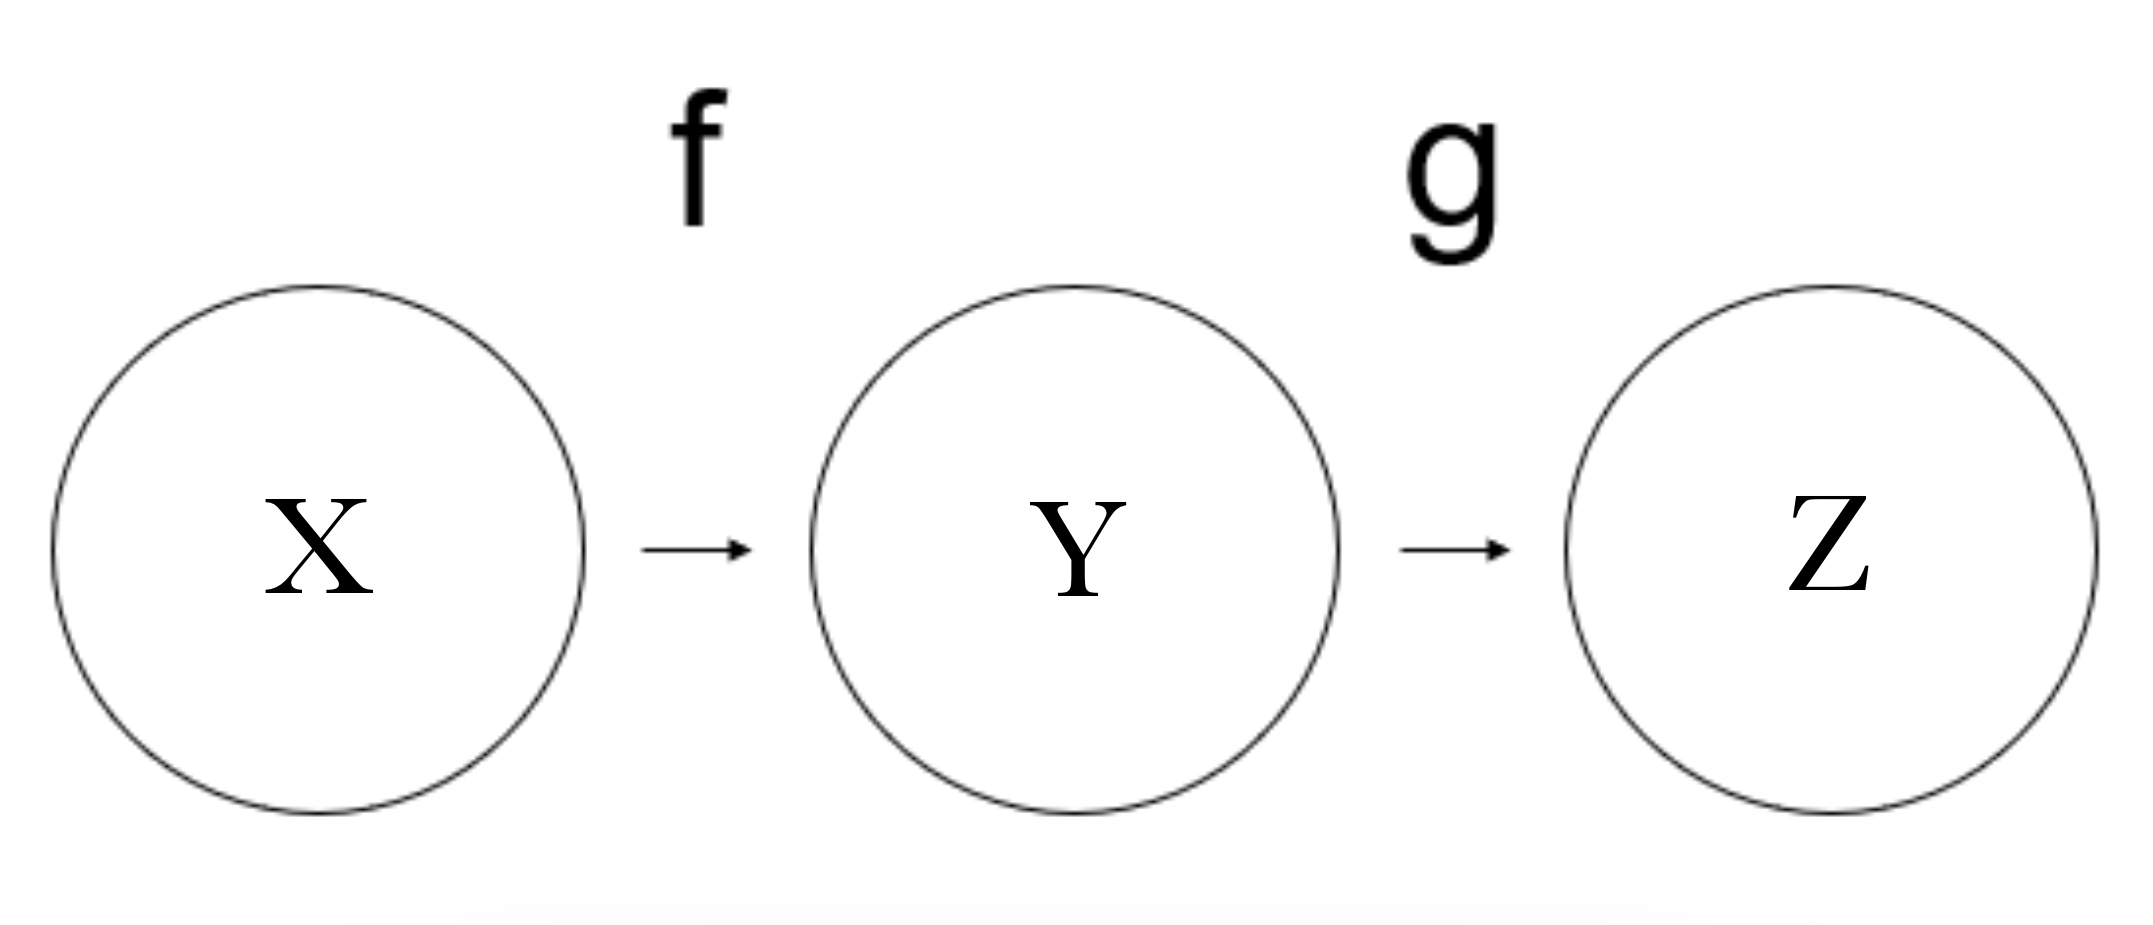
\includegraphics[width=0.4\linewidth]{IMG_1713.jpeg}
        \end{figure}
        Así, la composición es \(f \circ g : X \rightarrow Z\)
        \vspace{\baselineskip}
        
        P.D. \(\forall a, b \in X\), \((g \circ f)(a) = (g \circ f)(b)\) implica \(a = b\).
        
        \begin{proof} Sean \(a, b \in X\), supongamos \((g \circ f)(a) = (g \circ f)(b)\), por definición de la composición:
        
        \(g(f(a)) = g(f(b))\)
        \vspace{\baselineskip}
        
        Por ser \(g\) inyectiva, si dos entradas evaluadas son iguales, esas entradas son iguales:
        
        \(f(a) = f(b)\)
        \vspace{\baselineskip}
        
        Análogamente, por ser \(f\) inyectiva, se cumple:
        
        \(a = b\)
        \end{proof}
        \vspace{\baselineskip}

        \item[d)] Si \(f\) y \(g\) son funciones suprayectivas, entonces \(g \circ f\) es suprayectiva.
        
        La composición, una vez más, se ve como:
        \begin{figure}[H]
            \centering
            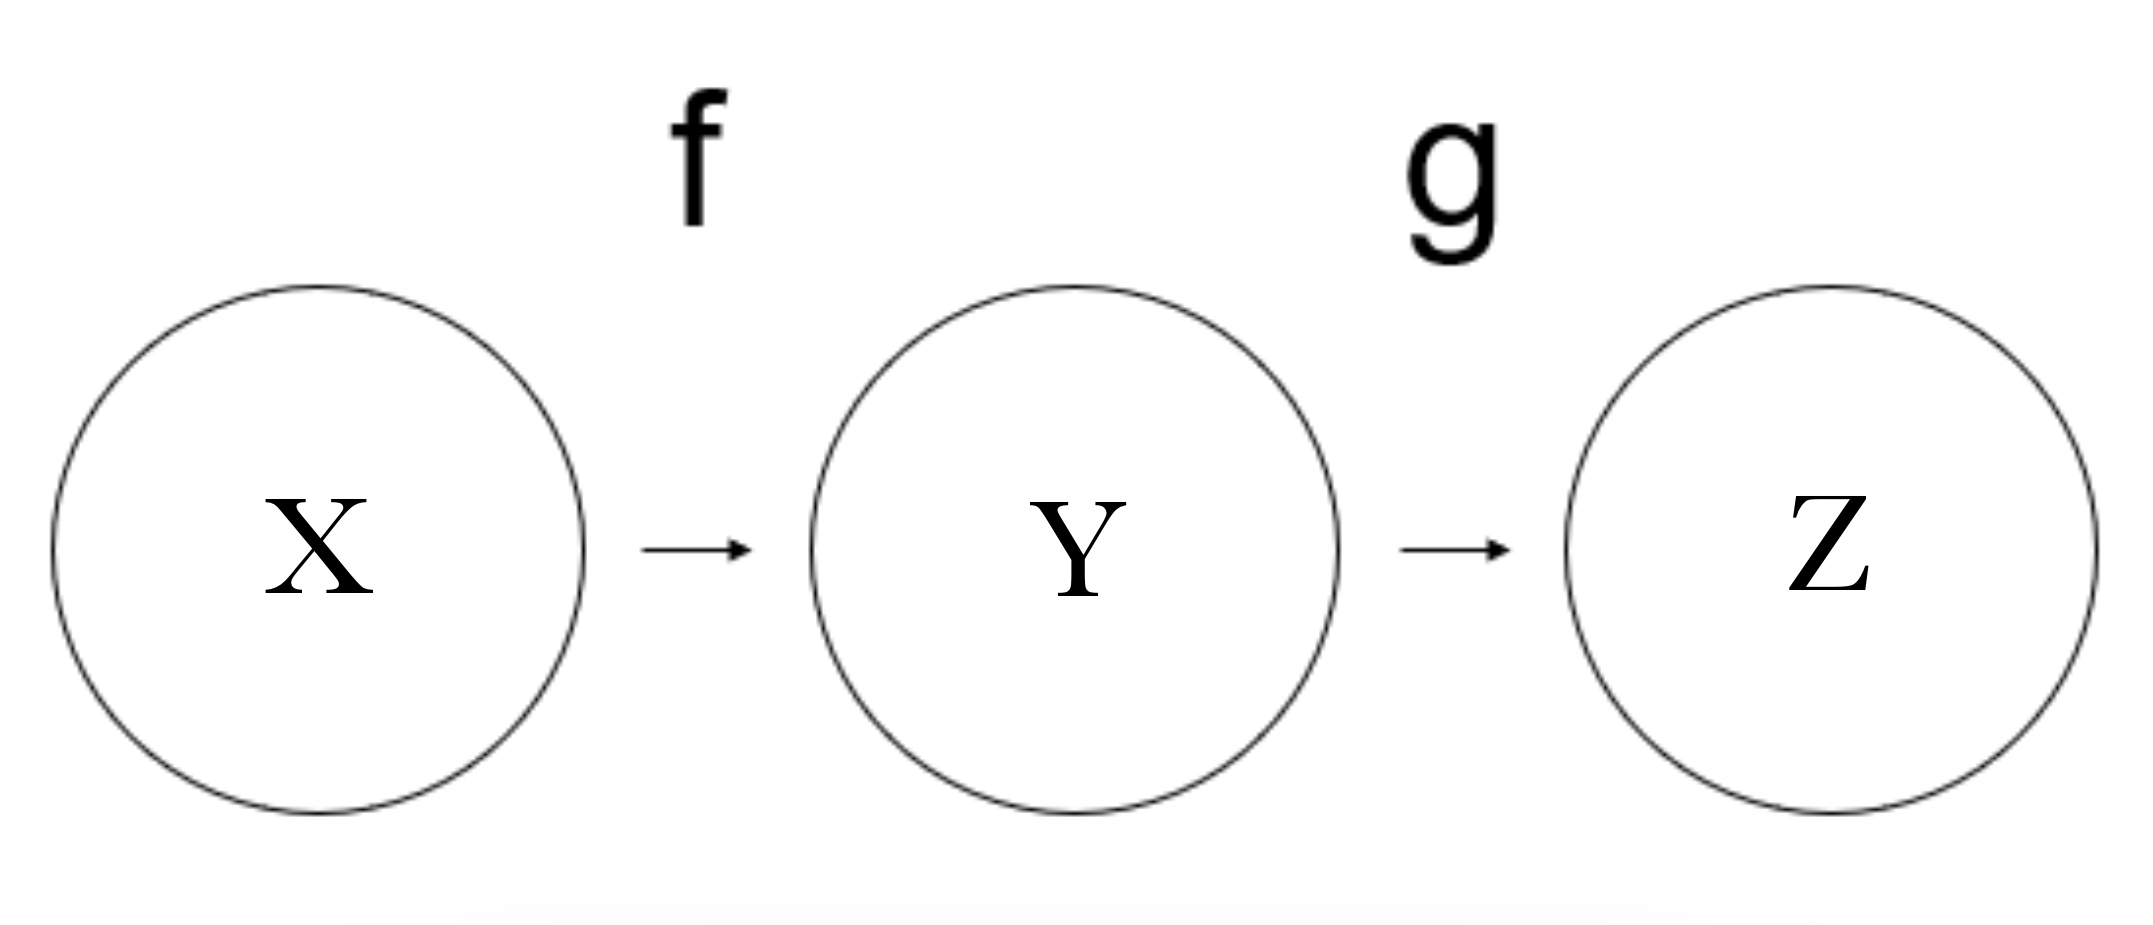
\includegraphics[width=0.4\linewidth]{IMG_1713.jpeg}
        \end{figure}
        \(g \circ f : X \rightarrow Z\)
        \vspace{\baselineskip}
        
        P. D. Sean \(f\) y \(g\) sobreyectivas, \(g \circ f\) es sobreyectiva.
        
        \(\Rightarrow \forall c \in Z\), \(\exists a \in X\) tal que \((g \circ f)(a) = c\).
        
        \begin{proof} Sea \(c \in Z\), entonces, por ser \(g\) sobreyectiva, existe \(b \in Y\) tal que \(g(b) = c\).
        \vspace{\baselineskip}
        
        Y, como existe ese \(b \in Y\), por ser \(f\) suprayectiva, entonces existe \(a \in X\) tal que \(f(a) = b\).
        \vspace{\baselineskip}
        
        Entonces:
        
        \(g(b) = c\)
        
        \(g(f(a)) = c\)
        
        \((g \circ f)(a) = c\)
        \end{proof}
    \end{enumerate}
\end{enumerate}

\end{document}
